\documentclass[accentcolor=tud1c, 11pt, toc=bib, toc=listof, captions=abovetable, parskip=half]{tudreport}
%********************************************
% Wichtige Pakete. Inputenc muss vor der Definition von \Thesisname geladen werden, sonst funktionieren Umlaute nicht,
% daher stehen die wichtigen Pakete hier und nicht in der Praeambel.tex
\usepackage[ngerman]{babel} %Sprachpaket, z.B. für Trennregeln
\usepackage{iftex}
\ifPDFTeX
	\usepackage[utf8]{inputenc} %Eingabeencoding (wichtig z.B. für Umlaute)
\else\fi

\definecolor{commentgreen}{RGB}{50,127,50}
\hbadness=100000

\usepackage{listings} \lstset{basicstyle=\footnotesize\ttfamily\fontseries{lc}\selectfont}
\renewcommand*\lstlistingname{Quelltext}
\lstset{columns=flexible,keywordstyle=\color{purple},stringstyle=\color{blue},commentstyle=\color{commentgreen},numberstyle=\tiny\color{gray},frame=single,numbers=left}

\usepackage{tikz}
\usetikzlibrary{arrows,decorations.pathreplacing}
\tikzset{cross/.style={path picture={
  \draw[red]
    (path picture bounding box.south east)--(path picture bounding box.north west)
    (path picture bounding box.south west)--(path picture bounding box.north east);
}}}
\usepackage{siunitx} 
\DeclareSIUnit\pixel{px}
\usepackage{amsmath}
\newcommand{\Mod}[1]{\ (\mathrm{mod}\ #1)}
\usepackage{commath}
\usepackage{multicol}
\usetikzlibrary{plotmarks}

\usepackage{algorithm}% http://ctan.org/pkg/algorithms
\usepackage{algpseudocode}% http://ctan.org/pkg/algorithmicx

\usepackage{pgfplots}
\pgfplotsset{compat=newest}
\pgfplotsset{major grid style={dashed}}

\usepackage{tabularx}
\usepackage{booktabs}
\usepackage{geometry}
\usepackage{subcaption}
\usetikzlibrary{calc,positioning}
%********************************************

\newcommand*{\Thesisname}	{Bachelorarbeit}
\newcommand*{\Vorname}		{Dimitri}
\newcommand*{\Nachname}		{Haas}
%********************************************
%Weitere wichtige Pakete
\usepackage{amsmath} %Formeln
\usepackage{graphicx} %Graphikformate
\usepackage{flafter} %Float-Umgebungen erscheinen frühestens nach ihrer Position im Quellcode
\usepackage{pdflscape} %Querseiten
\usepackage{booktabs} % Schöne Unterteilungsstriche für Tabellen: \toprule, \bottomrule
\usepackage{pdfpages} %pdf-Dateien ganzseitig einbinden -- Alternative zu \includegraphics
%*******************************************

%********************************************
% "Kann"-Pakete, jeder muss selbst entscheiden ob er sie verwenden möchte
%\usepackage{booktabs} %Schöne Unterteilungsstriche für Tabellen (\toprule, \bottomrule, \midrule,...)
\usepackage{siunitx} %Formatierung für Zahlen, Einheiten, Winkel,...
\usepackage[babel]{csquotes} %Sprachenspezifische Zitierregeln und Anführungszeichen, Paket wird auch für biblatex benötigt
\usepackage[style=numeric-comp, sorting=none, alldates=short, abbreviate=false, maxcitenames=2, maxbibnames=99, eprint=false, hyperref=auto, backend=biber]{biblatex} %Literaturverzeichnis, Achtung: Für backend=biber muss man auch biber statt bibtex benutzen! Mehr Informationen: http://biblatex-biber.sourceforge.net/
%\usepackage{icomma} %Komma ist Dezimaltrenner im Mathemodus
%\usepackage{tabu} % Etwas komfortablerer Tabellensatz
%\usepackage{multicol} %Mehrspaltiger Satz
%\usepackage{pgfplots} %Erstellt Plots von Funktionen oder Messwerten
%********************************************

%********************************************
% Hyperref wird sehr empfohlen, muss aber als letztes Paket eingebunden werden
\ifPDFTeX
	\usepackage[hyperfootnotes=false]{hyperref}
\else
	\usepackage[unicode]{hyperref}
\fi
\usepackage[all]{hypcap} %Verweise auf Floats (Abb., Tabellen) zeigen nicht auf die Bildunterschrift sondern auf das obere Ende des Bildes
%********************************************

%*********** Seitenlayout, TUD-Design *****************************************************
\geometry{left=35mm, right=20mm, top=20mm, bottom=20mm, nomarginpar, includeall} %Seitenränder EMK-konform setzen
\setinstitutionlogo{Figures/EMK_Logo}
%\printpicturesize %Gibt den verfügbaren Platz für das Titelbild auf der Titelseite aus, praktisch um ein Bild zurechtzuschneiden
%****************************************************************************

%********** Kopf- und Fußzeilen ***********************************************
\makeatletter
% Kopf- und Fußzeile für den Hauptteil
\fancypagestyle{headings}{%
    \fancyhf{} %Alle Kopf- und Fusszeilen abschalten
    \fancyhead[L]{\TUD@indentbar[\headwidth]} %Kopfzeile oben links ist TUD-Identitätsbalken über die gesamte Breite
		\fancyhead[R]{} %Kopfzeile rechts leer
    \fancyfoot[L]{\footerfont\strut\\\Thesisname\ -- \Nachname} %TBD Fußzeile links
		\fancyfoot[C]{\tudrule[\headwidth]\footerfont\strut\\\nouppercase\leftmark} %Überkapitel in der Fußzeile zentriert
		\fancyfoot[R]{\footerfont\strut\\\thepage} %Seitenzahl in der Fußzeile außen
  }
% Kopf- und Fußzeile für Kapitelseiten
\fancypagestyle{chapterheadings}{%
    \fancyhf{} %Alle Kopf- und Fusszeilen abschalten
    \fancyhead[L]{\TUD@indentbar[\headwidth]} %TUD-Identitätsbalken
		\fancyhead[R]{}
    \fancyfoot[L]{\footerfont\strut\\\Thesisname\ -- \Nachname} %TBD Fußzeile links
		\fancyfoot[C]{\tudrule[\headwidth]\footerfont\strut\\\nouppercase\leftmark} %Überkapitel in der Fußzeile zentriert
		\fancyfoot[R]{\footerfont\strut\\\thepage} %Seitenzahl in der Fußzeile außen
  }
%Kopf- und Fußzeile für die Zusammenfassung
\fancypagestyle{zusammenfassung}{%
	\fancyhf{} %Alle Kopf- und Fusszeilen abschalten
	\fancyhead[L]{\TUD@indentbar[\headwidth]} %TUD-Identitätsbalken
	\fancyfoot[C]{\tudrule[\headwidth]\footerfont\strut\\\Thesisname\ -- \Nachname\\Institut EMK -- TU Darmstadt}
}

\@ifundefined{chapter}{}{ %falls \chapter existiert, wird das folgende ausgeführt
	\renewcommand*{\chapterpagestyle}{headings} %Kopf- und Fußzeilen auch auf Seiten, auf denen ein neues Kapitel beginnt
}
\makeatother
%****************************************************************************

%*************** Automatische Positionierung von Floatobjekten (Bildern, Tabellen, etc.)*************
% siehe http://projekte.dante.de/DanteFAQ/FloatPlatzierung
\makeatletter
\renewcommand{\fps@figure}{htbp} %Standardplatzierungsoption für figures auf htbp ändern
\renewcommand{\fps@table}{htbp} %Standardplatzierungsoption für tables auf htbp ändern
\makeatother
\setcounter{topnumber}           {3} %Maximale Anzahl Floatobjekte oben auf einer Seite (t), Standard 2
\setcounter{bottomnumber}        {1} %Maximale Anzahl Floatobjekte unten auf einer Seite (b), Standard 1
\setcounter{totalnumber}         {4} %Maximale Anzahl Floatobjekte gesamt auf einer Seite, Standard 3
\renewcommand{\floatpagefraction}{0.8} %Minimaler Seitenanteil für Platzierung page (p), Standard 0.5
\renewcommand{\topfraction}      {0.9} %Maximaler Seitenanteil der für Platzierung top (t) verwendet werden darf, Standard 0.7
\renewcommand{\bottomfraction}   {0.6} %Maximaler Seitenanteil der für Platzierung bottom (b) verwendet werden darf, Standard 0.3
\renewcommand{\textfraction}     {0.15} %Minimaler Seitenanteil Text auf einer Seite, Standard 0.2
%*******************************************************************************

%*************hyperref*************************************************
\hypersetup{pdfauthor={\Vorname \Nachname}}
\addto\extrasngerman{%
	\renewcommand{\appendixautorefname}{\appendixname}
	\renewcommand{\sectionautorefname}{Kapitel}
	\renewcommand{\subsectionautorefname}{Kapitel}
}
% Hack von Heiko Oberdieck in de.comp.text.tex, damit autoref bei Verweisen sowohl auf Kapitel als auch auf Unterkapitel im Anhang immer schreibt "siehe Anhang xy"
% Suchbegriff bei google: in:de.comp.text.tex Autoref im Anhang
\makeatletter
\@ifundefined{chapter}{}{
	\newcommand*{\theappendix}{\thechapter}
	\newcommand*{\theHappendix}{%
		\number\value{chapter}.\number\value{section}%
	}
	\let\org@hyper@makecurrent\hyper@makecurrent
	\def\string@section{section}
	\def\hyper@makecurrent#1{%
		\expandafter\ifx\@chapapp\appendixname
			\def\string@temp{#1}%
			\ifx\string@section\string@temp
				\org@hyper@makecurrent{appendix}%
			\else
				\org@hyper@makecurrent{#1}%
			\fi
		\else
			\org@hyper@makecurrent{#1}%
		\fi
	}
}
\makeatother
%**********************************************************************

%********** biblatex, csquotes ********************************************************
\MakeOuterQuote{"}
\DefineBibliographyStrings{ngerman}{
	andothers={et\ \addabbrvspace al\adddot},
	urlseen={abgerufen am}
	}
\renewcommand*{\mkbibnamelast}[1]{\textsc{#1}} %Autorennamen in Kapitälchen
\renewcommand*{\multinamedelim}{\addsemicolon\space} % Namen im Literaturverzeichnis mit Semikolon getrennt
\DeclareNameAlias{default}{last-first} % Bei Namen Nachname zuerst
% Nachnamen, dann Vornamen abgekürzt
%\DeclareNameFormat{labelname}{%
  %\usebibmacro{name:last-first}{#1}{#4}{#6}{#8}%
  %\usebibmacro{name:andothers}}
%\DeclareNameFormat{sortname}{%
  %\usebibmacro{name:last-first}{#1}{#4}{#6}{#8}%
  %\usebibmacro{name:andothers}} 
% Wesentlicher Titel immer kursiv. Buchtitel, Journaltitel, etc. in Anführungszeichen.
\DeclareFieldFormat{journaltitle}{\mkbibquote{#1\isdot}}
\DeclareFieldFormat{maintitle}{\mkbibquote{#1\isdot}}
\DeclareFieldFormat{booktitle}{\mkbibquote{#1\isdot}}
\DeclareFieldFormat[article]{title}{\mkbibemph{#1}}
\DeclareFieldFormat[inbook]{title}{\mkbibemph{#1}}
\DeclareFieldFormat[incollection]{title}{\mkbibemph{#1}}
\DeclareFieldFormat[inproceedings]{title}{\mkbibemph{#1}}
\DeclareFieldFormat[patent]{title}{\mkbibemph{#1}}
\DeclareFieldFormat[thesis]{title}{\mkbibemph{#1}} 
%****************************************************************************

%********* siunitx ***************************************************
\sisetup{redefine-symbols=false,
			detect-all,
			text-micro={{\normalfont\textmu}},
			math-micro={\mbox{\normalfont\textmu}},
}
\addto\extrasngerman{
	\sisetup{
	locale=DE
	}
}
%**********************************************************************
%\settitlepicture{TBD} %Bild auf der Titelseite

\begin{document}
\title{Oberflächenbestimmung von Nanodrähten durch Bildverarbeitung}
\subtitle{von \Vorname\ \Nachname}
\subsubtitle{\Thesisname, vorgelegt im November 2018\\Betreuer: Konja Wick, M.Sc.\\Institut für Elektromechanische Konstruktionen}
	
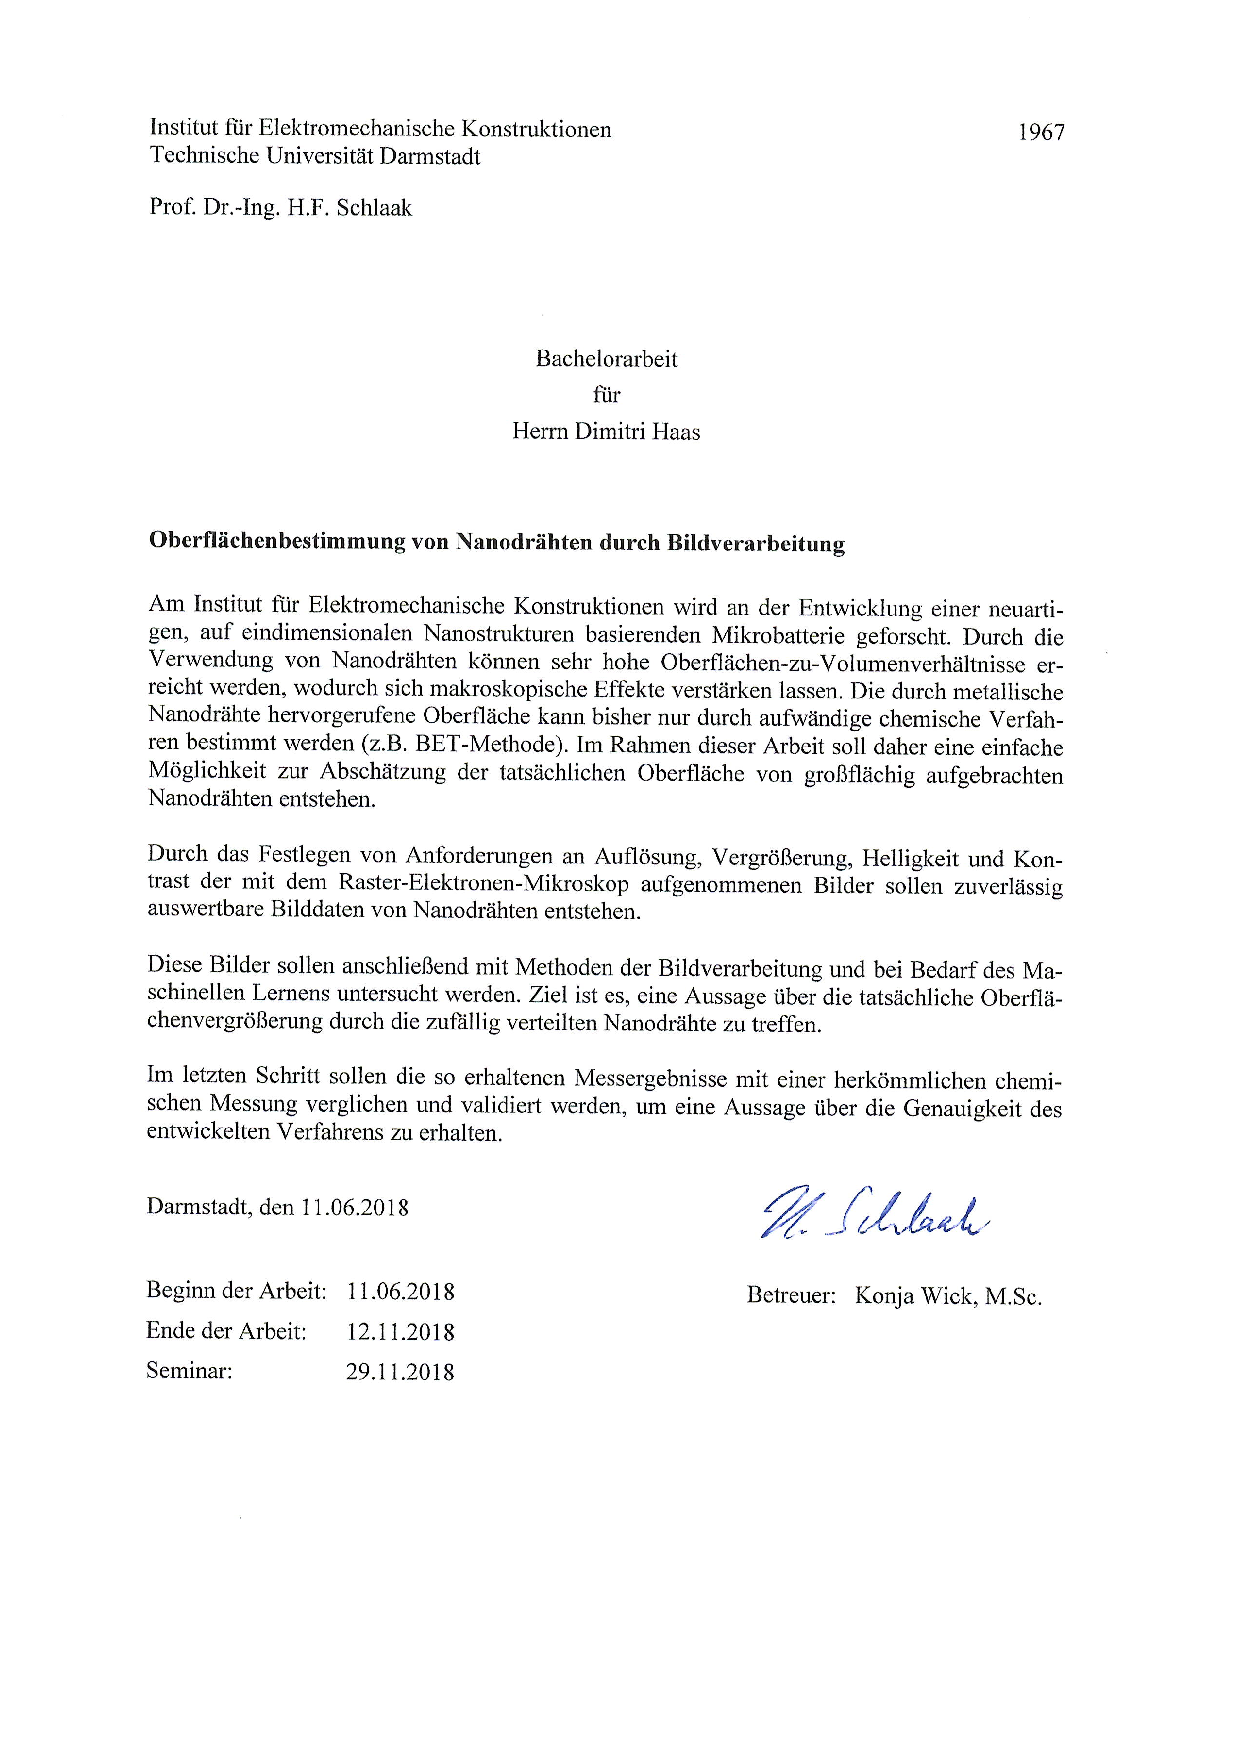
\includepdf[pagecommand={\thispagestyle{realempty}}]{ExternalFiles/EMKTemplate/OffizielleAufgabenstellung}
\maketitle
\pagenumbering{Roman} 
\begingroup
\chapter*{Erklärung zur Abschlussarbeit gemäß § 22 Abs. 7 und § 23 Abs. 7 APB TU Darmstadt}
	\thispagestyle{empty}
%	\accentfont\large
	\parindent0em
%	\vskip2ex
		Hiermit versichere ich, \Vorname\ \Nachname, die vorliegende \Thesisname\ gemäß § 22 Abs. 7 APB der TU Darmstadt ohne Hilfe Dritter und nur mit den angegebenen Quellen und Hilfsmitteln angefertigt zu haben. Alle Stellen, die Quellen entnommen wurden, sind als solche kenntlich gemacht worden. Diese Arbeit hat in gleicher oder ähnlicher Form noch keiner Prüfungsbehörde vorgelegen. 
		Mir ist bekannt, dass im Falle eines Plagiats (§38 Abs.2 APB) ein Täuschungsversuch vorliegt, der dazu führt, dass die Arbeit mit 5,0 bewertet und damit ein Prüfungsversuch verbraucht wird. Abschlussarbeiten dürfen nur einmal wiederholt werden.
		Bei der abgegebenen Thesis stimmen die schriftliche und die zur Archivierung eingereichte elektronische Fassung gemäß § 23 Abs. 7 APB überein.
		Bei einer Thesis des Fachbereichs Architektur entspricht die eingereichte elektronische Fassung dem vorgestellten Modell und den vorgelegten Plänen.\\
		
		\rule{0.7\textwidth}{0.4pt}\\
		
		\textbf{English translation for information purposes only:}\\
		\textbf{Thesis Statement pursuant to § 22 paragraph 7 and § 23 paragraph 7 of APB TU Darmstadt}\\
		I herewith formally declare that I, \Vorname\ \Nachname, have written the submitted thesis independently pursuant to § 22 paragraph 7 of APB TU Darmstadt. I did not use any outside support except for the quoted literature and other sources mentioned in the paper. I clearly marked and separately listed all of the literature and all of the other sources which I employed when producing this academic work, either literally or in content. This thesis has not been handed in or published before in the same or similar form.
		I am aware, that in case of an attempt at deception based on plagiarism (§38 Abs. 2 APB), the thesis would be graded with 5,0 and counted as one failed examination attempt. The thesis may only be repeated once.
		In the submitted thesis the written copies and the electronic version for archiving are pursuant to § 23 paragraph 7 of APB identical in content.
		For a thesis of the Department of Architecture, the submitted electronic version corresponds to the presented model and the submitted architectural plans.
		
	\vskip5ex
		Darmstadt, den 12. November 2018
	\vskip6ex
	\tudrule[0.5\textwidth]\\
		{\normalsize(\Vorname\ \Nachname)}
\endgroup
\pagestyle{headings} %Kopf- und Fußzeile an
\setcounter{tocdepth}{2} %Tiefe des Inhaltsverzeichnisses

\clearpage %muss hier stehen sonst klappt die Umschaltung der Seitennummerierung nicht
\pagenumbering{arabic}
	
% TBD HIER KOMMT DER INHALT HIN
\begin{abstract}
Ziel dieser Arbeit ist die Entwicklung einer Methode zur Abschätzung der Oberflächenvergrößerung durch großflächig aufgebrachte Nanodrähte anhand auswertbarer Bilddaten eines Rasterelektronenmikroskops. Untersucht wurden dabei die Poren von sogenannten Templatfolien, welche zur galvanischen Erzeugung von Mikro- und Nanodrähten benötigt werden. Durch ausreichende Vergrößerung der auflaminierten Folie konnten Position und Verlauf der Poren mittels Techniken der Bildverarbeitung erfasst und ein Rückschluss auf die Mantelfläche der anschließend erzeugten Drähte gezogen werden.\\

Mithilfe der Software \textsc{Matlab} und des dazugehörigen Plug-Ins \textit{Image Processing Toolbox} wurden im ersten Schritt die Aufnahmen durch Zuschnitt und Skalierung für die weitere Verarbeitung adaptiert. Darauf folgte die Untersuchung und Anwendung zweier Methoden der Informationsgewinnung im Rahmen der Kanten- und Kreisdetektion.\\
Erstere projiziert mittels Hough-Transformation gefundene Kreise auf die Aufenthaltsorte der Poren und berechnet in einem geometrischen Kontext die gesamte Umfangslinie. Erschwerend kam hinzu, dass diese Poren nicht ausschließlich isoliert auf der Oberfläche vorliegen, sondern sich beliebig überschneiden können. Auf den daraus entstehenden trigonometrischen Rechenaufwand wird detailliert eingegangen. \\
Mit dem Ziel die Berechnung zu beschleunigen, wurde als zweite Möglichkeit die durch den Canny Algorithmus extrahierte Kontur und deren Pixelanzahl als Annäherung für Länge und Aufenthaltsort der Umfangslinie vorgestellt. Die resultierenden Messabweichungen werden mithilfe von Streugrößen auf Systematik und die Möglichkeit einer Kompensation anhand vieler Fallbeispiele untersucht.\\
Die aus beiden Methoden gewonnene Umfangslinienlänge wird in einem letzten Schritt zur Bestimmung der Mantelfläche und der damit verbundenen Oberflächenvergrößerung genutzt.\\

In einer Gegenüberstellung wurden anschließend Zeitperformance, Robustheit bezüglich unterschiedlicher Aufnahmeparameter und die geschätzte Mantelfläche beider Methoden miteinander verglichen. Hierbei überzeugte vor allem die geometrische Methode mit einer präzisen Kreisdetektion und -lokalisation, wodurch eine genaue Berechnung der Oberflächenvergrößerung möglich war. Negativ hat sich zum Teil nur die Ausführungszeit von bis zu zwei Minuten ausgewirkt, wenn der für den Algorithmus benötigte Sensitivitätswert noch generisch berechnet werden musste. Aufgrund der genauen Ergebnisse der geometrischen Berechnung, wurden diese als Referenzwert für die Beurteilung der pixelbasierten Methode verwendet. Schlussfolgerend konnte festgestellt werden, dass die pixelbasierte Methode um den Faktor 20-30 schneller arbeitet als ihr geometrischer Pendant – sich jedoch nicht besonders robust gegenüber unterschiedlichen Bildparametern zeigt. Die Schwächen liegen insbesondere in niedrigen Auflösungen und kleinen Abbilungsmaßstäben der REM-Aufnahmen. Messunsicherheiten sind deshalb nicht ohne weiteres vernachlässigbar.\\

Die Arbeit schließt mit einem Ausblick auf weitere, mögliche Ansatzpunkte zur Erhöhung der Genauigkeit und Performance der Oberflächenbestimmung.
\end{abstract}

\tableofcontents %Inhaltsverzeichnis erstellen

\chapter{Einleitung}
Am Institut für Elektromechanische Konstruktionen der TU Darmstadt wird an der Entwicklung einer neuartigen, auf eindimensionalen Nanostrukturen basierenden Mikrobatterie geforscht. Durch die Verwendung von Nanodrähten können sehr hohe Oberflächen-zu-Volumenverhältnisse erreicht werden, wodurch sich makroskopische Effekte verstärken lassen. Die durch metallische Nanodrähte hervorgerufene Oberfläche kann bisher nur durch aufwändige chemische Verfahren bestimmt werden (z.B. BET-Methode). Im Rahmen dieser Arbeit soll daher eine einfache Möglichkeit zur Abschätzung der tatsächlichen Oberfläche von großflächig aufgebrachten Nanodrähten entstehen.

Durch das Festlegen von Anforderungen an Auflösung, Vergrößerung, Helligkeit und Kontrast der mit dem Raster-Elektronen-Mikroskop aufgenommenen Bilder, sollen zuverlässig auswertbare Bilddaten von Nanodrähten generiert werden können.

Diese Bilder sollen anschließend mit Methoden der Bildverarbeitung untersucht werden. Ziel ist es, eine Aussage über die tatsächliche Oberflächenvergrößerung der zufällig verteilten Nanodrähte zu treffen. 

\section{Motivation}
Die Bestimmung der aktiven Oberfläche eines Nanodraht-Arrays ist in der Regel mit einem chemischen Messverfahren \footnote{Die Oberfläche lässt sich beispielsweise mithilfe der \emph{Cyclovoltammetrie} [6] abschätzen. Dies ist ein analytisches Verfahren, mit dessen Hilfe man Elektrodenprozesse beobachtet und Ausschläge in der Widerstandskennlinie in direkten Zusammenhang mit der chemisch aktiven Oberfläche setzt.} verbunden, das in einem Labor durchgeführt werden muss. Damit geht eine terminliche und personelle Vorbereitung sowie ein filigraner Versuchssaufbau einher, der die Berücksichtigung von Messunsicherheiten und den Umstand mehrerer Anläufe nötig macht. Dies resultiert in einem hohen Zeit- und Kostenfaktor für den Ingenieur.\\
Aus diesem Grund ist es besonders interessant im Rahmen dieser Arbeit ein Verfahren zu entwickeln, mit dessen Hilfe sich die Abschätzung der Array-Oberfläche deutlich beschleunigen lässt.
 
Die Anfertigung von Aufnahmen mit einem Rasterelektronenmikroskop lassen sich vergleichsweise schnell anfertigen. Sind die gewünschten Aufnahmeparameter eingestellt, können viele Bilder in kurzer Zeit aufgenommen und gespeichert werden. Diese Bilder können von da an automatisiert vom Rechner mithilfe verschiedenster Techniken aus der Disziplin \emph{Computer Vision} gesichtet, analysiert und ausgewertet werden. Eine abschätzende Aussage zur Oberflächenvergrößerung kann auf diese Weise innerhalb weniger Sekunden bis wenigen Minuten getroffen und zur weiteren Beurteilung herangezogen werden. Eine einzige Oberflächenmessung im Labor kann dagegen nicht selten bis zu einer Stunde dauern.

\section{Gliederung der Arbeit}
Die Arbeitsschritte zur Extraktion von Informationen aus einem Bild im Rahmen der Bildverarbeitung umfassen in dieser Arbeit die Aufbereitung des Bildes in Kapitel \ref{ch:preprocessing}, die Extraktion der Kanten in Kapitel \ref{ch:kantendetektion}, die Suche nach geometrischen Kreisen in Kapitel \ref{ch:kreisdetektion} und die anschließende  Berechnung der geometrischen Oberfläche der zu untersuchenden Struktur in Kapitel \ref{sec:geomUmfangsberechnung}.\\

Dabei werden zwei Ansätze der Oberflächenerfassung verfolgt:
\begin{enumerate}
\item \textbf{Kreisdetektion mithilfe von Hough-Transformation und der MATLAB-Funktion imfindcircles}\\
Wenn mehr Rechenzeit zur Verfügung steht, soll eine genauere Variante mit Hilfe der Hough-Transformation [1] durchgeführt werden. Dabei wird das Bild nach kreisähnlichen Strukturen abgesucht und bei jedem Treffer ein idealer Kreis an der jeweiligen Position angenommen. Da sich diese auch überschneiden und damit kleinere Mantelflächen zur Folge haben können, müssen die genauen Positionen der Kreise zwischengespeichert und geometrisch untersucht werden. Dies wird in Abschnitt \ref{sec:geomUmfangsberechnung} näher beleuchtet.
\item \textbf{Analyse der detektierten Kanten}\\
In dieser Methode wird das Bild auf seine Kanten und Konturen untersucht, um diese anschließend als Grundlage für eine Oberflächenberechnung heranzuziehen. Als Kantenfilter wird der sogenannte Canny-Filter [2] näher untersucht, da dieser heute als der profilierteste Kantenfilter gilt. Anhand der Anzahl der detektierten Pixel wird die Länge des Umrisses unter Berücksichtigung des Diskritisierungsfehlers durch Kreisrasterung abgeschätzt. Dieser Umriss kann in einem weiteren Schritt zur Berechnung der Mantelfläche herangezogen werden. Dieser Ansatz wird ab Abschnitt \ref{pixelbasierteUmfangsberechnung} behandelt.
\end{enumerate}
Nach Vorstellung beider Abschätzungsverfahren werden diese in Kapitel \ref{ch:vergleichDerErgebnisse} auf ihre Performance, Zuverlässigkeit und Fehlerkorrelation untersucht. 

\section{Werkzeuge}
Für die Aufgabenstellung eignet sich eine Vielzahl von Werkzeugen und Programmiersprachen. Gut dokumentierte Frameworks zur Bildverarbeitung gibt es beispielsweise für Python (\textit{OpenCV} [7]) und \textsc{Matlab} (\textit{Image Processing Toolbox} [8]).\\

In dieser Arbeit wird das Problem in erster Linie mit \textsc{Matlab} in der Version \lstinline|R2017b| gelöst. Dabei werden robuste, vorimplementierte  Funktionen wie beispielsweise \lstinline|imfindcircles| genutzt, welche mit Hilfe der Hough-Transformation hervorragende Ergebnisse hinsichtlich der detektierten Kreise zeigen. Die generische Bestimmung möglichst idealer Parameter zur Steuerung dieser Funktionen bildet einen wesentlichen Teil dieser Arbeit.\\

Weiter wird auch die Auswirkung unterschiedlicher Aufnahme- und Bildparameter auf das Ergebnis und die Performance der hier vorgestellten Berechnungsmethoden betrachtet.

\section{Auswahl der zu untersuchenden Bildern}
Vor Beginn der Untersuchung der Oberfläche stellt sich die Frage, ob die Analyse von vornerein durch eine gezielte Auswahl von Bildern positiv beeinflusst werden kann. So kann sowohl eine Aufnahme der Nanodrähte (Abb. \ref{fig:remScharf1}) als auch die einer Templatfolie (Abb. \ref{fig:remScharf2}) als Ausgangsmaterial für die Berechnung in Betracht gezogen werden. Vorangegangene Kantendetektionen haben gezeigt, dass die Aufnahmen von Drähten eine Oberflächenberechnung sehr erschweren. Das liegt vor allem daran, dass die Querschnittsflächen der Drähte, welche nicht orthogonal zum Betrachter zeigen, optisch mit einem großen Teil ihrer Mantelfläche verschmelzen (in Abb. \ref{fig:remScharf1Edge} an vielen diagonal verlaufenden Bildern sichtbar) und damit eine Abgrenzung beider Flächenanteile sehr schwierig ist.\\

Aus diesem Grund werden vorrangig nur Aufnahmen von Templatfolien untersucht, da die Abgrenzungen der Poren auch nach der Kantendetektion weitestgehend erhalten bleiben (siehe Abb. \ref{fig:remScharf2Edge}).\\

\begin{figure}[h!]
    \centering
    \begin{subfigure}[b]{0.475\textwidth}
        \centering
        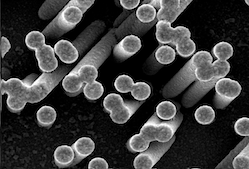
\includegraphics[scale=0.8]{Figures/remScharf.png}
        \caption{Aufnahme mehrerer Nanodrähte mit einem Rasterelektronenmikroskop}
        \label{fig:remScharf1}
    \end{subfigure}
    \hfill
    \begin{subfigure}[b]{0.475\textwidth}
        \centering
        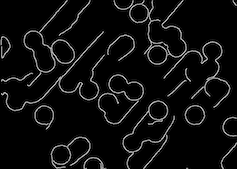
\includegraphics[scale=0.77]{Figures/remScharfEdge.png}
        \caption{Extraktion der Kanten mithilfe des Canny Algorithmus}
        \label{fig:remScharf1Edge}
    \end{subfigure}
    \caption{Anhand des Kantenbilds eines Nanodrahtarrays wird ersichtlich, dass Flächendiskontinuitäten nicht immer von einem Kantenfilter erfasst werden können. }
\end{figure}
\quad
\begin{figure}[h!]
    \centering
    \begin{subfigure}[b]{0.475\textwidth}
        \centering
        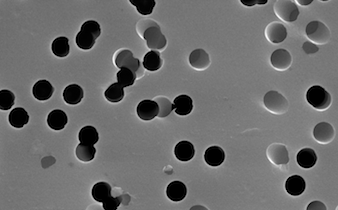
\includegraphics[scale=0.53]{Figures/remScharf2.png}
        \caption{REM-Aufnahme einer auflaminierten Templatfolie mit gut sichtbaren Poren}
        \label{fig:remScharf2}
    \end{subfigure}
    \hfill
    \begin{subfigure}[b]{0.475\textwidth}
        \centering
        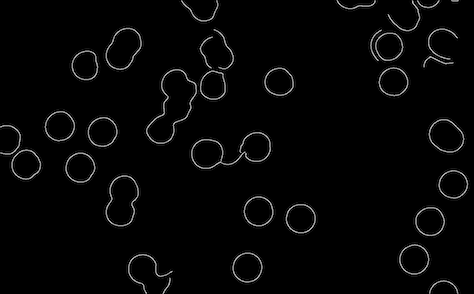
\includegraphics[scale=0.38]{Figures/remScharf2Edge.png}
        \caption{Auch hier fand eine Kantenextraktion durch den Canny Filter statt}
        \label{fig:remScharf2Edge}
    \end{subfigure}
    \caption{Verglichen zu Abb. \ref{fig:remScharf1} lassen sich Umfangslinien einzelner Löcher deutlich besser extrahieren, da ein ausreichender Kontrast zwischen den aufeinandertreffenden Flächen vorliegt.}
\end{figure}
	
\chapter{Vorbereitung der REM-Aufnahmen}
\label{ch:preprocessing}
\section{Bildzuschnitt}
Bei den uns zur Verfügung stehenden Bilder handelt es sich um Aufnahmen aus einem Elektronenmikroskop. Diese werden im .tif-Format mit einer Auflösung von $1424\times968$ exportiert und gespeichert. Zusätzliche Meta-Informationen, wie beispielsweise Zoomfaktor, Auflösung, Helligkeit, Kontrast, angelegte Spannung und ein Maßbalken, werden mithilfe einer schwarzen Box am unteren, linken Rand des Bildes angezeigt. Diese Box überdeckt einen Teil des Bildes und muss deshalb vor der Untersuchung ausgeschnitten und bei Bedarf ausgelesen werden. Dieser Wegschnitt resultiert in einem etwas kleineren Bildausschnitt.\\

Für den in Abschnitt \ref{sec:kalibrierungsfaktor} berechneten Skalierungsfaktor sind die wichtigsten Parameter die Länge des Maßbalkens in Pixeln und der daneben aufgedruckte Wert in Mikrometern. Dieser Maßstab wird im betreffenden Abschnitt zur Berechnung des Skalierungsfaktors herangezogen. Dieser Faktor gibt an, wie viel die Länge eines Pixels in Mikrometern beträgt und ermöglicht damit erst die sinnvolle Einheitenkonvertierung.

Da die schwarze Infobox stets zum Gesamtbild die gleiche, relative Größe besitzt und an der gleichen, relativen Stelle lokalisiert ist, kann der Wegschnitt im Vorfeld festgelegt und mit einer einzelnen Zeile durchgeführt werden (s. Quelltext \ref{cutblackbox}).\\

\begin{lstlisting}[language=MATLAB, caption=Wegschnitt der schwarzen Infobox, label=cutblackbox]
A = A(1:floor(end*0.85),:);
\end{lstlisting}

\section{Anpassung der Auflösung}
Um bereits eine im Laufe dieser Arbeit entstandene Erkenntnis vorzugreifen: Hoch aufgelöste Bilder können wesentlich besser auf Strukturen untersucht werden. Deshalb ist es wünschenswert die Auflösung gegebenenfalls anzupassen, wenn diese aufgrund von niedriger Auflösung bildverarbeitende Techniken erschweren.\\
In \textsc{Matlab} können Bilder mit dem Befehl \lstinline|imresize| beliebig in verschiedene Richtungen skaliert werden. In Quelltext \ref{lst:imageresizing} wird das Bild \lstinline|Image| zunächst um \SI{5}{\percent} in $x$-Richtung gestaucht und anschließend um den Faktor 2 aufgebläht.\\

\begin{lstlisting}[language=MATLAB, caption=Bildskalierung in \textsc{Matlab}, label=lst:imageresizing]
[rows, columns] = size(Image);
scale = 2;
xScale = 0.95;
scaledImage = imresize(imresize(I,[rows columns*xScale]),scale);
\end{lstlisting}

Die in dieser Arbeit untersuchten REM-Bilder werden im Vorfeld um \SI{5}{\percent} in $x$-Richtung gestaucht\footnote{Damit wird die leichte Verzerrung des Bildes ausgeglichen, welche speziell bei diesem Rasterelektronenmikroskop auftraten.} und anschließend um den Faktor $1,4$ skaliert, um Bildgrößen von etwa $1000\times2000$ zu erhalten\footnote{Aus mehreren Versuchsreihen wurde ersichtlich, dass eine Auflösung von etwa $1000\times2000$ ein guter Kompromis zwischen guter Detektion und Rechenaufwand darstellt.}.\\

\section{Distanzmessung im Bild: Bestimmung des Skalierungsfaktors}
\label{sec:kalibrierungsfaktor}
Um herauszufinden, wie viele Mikrometer einem Pixel des zu analysierenden Bildes entsprechen, muss  der Skalierungsfaktor $S$ bestimmt werden, welcher die Umrechnung von Pixeln in Mikrometern ermöglicht.

\paragraph{Möglichkeit 1: Maßbalken ablesen}
Oft sind (mikroskopischen) Bildern ein Maßbalken beigefügt, an dessen Länge man den Maßstab ablesen kann. Um diesen Balken auslesen zu können, kann beispielsweise mit \textit{Template-Matching} [5] gearbeitet werden. Dazu wird eine Bilddatei eines weißen Balkens angelegt, damit diese als Template im Zielbild gesucht werden kan. Der Template-Matching-Algorithmus sucht das komplette Bild nach dem Brut-Force-Prinzip ab, bis das Template lokalisiert ist. Nach anschließender Pixelzählung des gefundenen Balkons, kann letztendlich der danebenstehende Zahlenwert mit den erfassten Pixeln in Relation gebracht und ein Skalierungsfaktor $S$ gebildet werden.\\

\begin{equation}
S := \frac{l_T}{l_M}
\label{eq:skalierungsfaktor}
\end{equation}

\textbf{Beispiel:} Beträgt die Länge $l_M$ des Maßbalkens \SI{160}{Pixel}, welche laut nebenstehendem Zahlenwert $l_T$ einer Länge von $\SI{2}{\micro\metre}$ entspricht, so liegt der Skalierungsfaktor nach Gleichung \ref{eq:skalierungsfaktor} bei $\frac{2}{160}$.
Wenn also nun eine Kantenlänge $l_{\text{px}}$ in Pixeln im Bild auf die echte Länge $l$ in Mikrometern untersucht werden soll, muss diese lediglich mit dem Skalierungsfaktor multipliziert werden:\\

\begin{equation}
l = l_{\text{px}} \cdot S 
\label{eq:echteLänge}
\end{equation}

\paragraph{Möglichkeit 2: Auslesen eines vorliegenden Datenblatts}
Wenn die Kreise eine bereits bekannte Größe (durch Vorliegen eines Datenblatts) haben, kann dies bei der Lokalisierung im Bild als Information zur Bestimmung des Skalierungsfaktors genutzt werden.\\

\textbf{Beispiel: Bestimmung eines Skalierungsfaktor anhand Datenblatt}\\ 
Anhand des Templat-Datenblatts werden Löcher mit einem Radius $r_{\text{D,px}}$ von \SI{200}{\nano\metre} erwartet. Werden nach Durchlaufen eines Such-Algorithmus Kreise mit einem durchschnittlichen Radius von \SI{27.6}{Pixeln} detektiert, so kann dieser mit $r_{\text{D,px}}$ zum Skalierungsfaktor $S = \frac{\SI{200}{\nano\metre}}{\SI{27.6}{px}} \approx \SI{7.25}{\frac{\nano\metre}{px}}$ verknüpft werden. \\

Da die meisten Aufnahmen mit der gleichen Zoomstufe aufgenommen wurden, kann der Vorgang des Template-Matchings ausgelassen und die Zoomstufe direkt beim Funktionsaufruf der Oberflächenberechnungsfunktion einbezogen werden. In einer Lookup-Tabelle können Zoomstufe und der Skalierungsstufe festgehalten und bei Bedarf herangezogen werden. Eine Lookup-Tabelle, wie sie  im Rahmen dieser Arbeit verwendet wurde, kann Tabelle \ref{tab:lookup} entnommen werden. \\

\begin{table}[h!]
	\caption{Lookup Table für unterschiedliche Skalierungsfaktoren}
	\centering
	\begin{tabular}{cc}
		\toprule
		Zoomstufe				&$S \left( \SI{}{\frac{\micro\metre}{px}}\right) $	\\
		\midrule
			$8000\times	$		&0.0219				\\
			$15000\times$		&0.0120				\\
			$20000\times$		&0.0088				\\
			$25000\times$		&0.0071				\\
			$65000\times$		&0.0027				\\
			$z \times$			&$\frac{175.2}{z}$	\\
		\bottomrule
	\end{tabular}
	\label{tab:lookup}
\end{table}

\chapter{Kanten- und Kreisdetektion: Informationsextraktion}
\label{ch:kreisdetektion}

\section{Hough-Transformation für Kreise}
In diesem Kapitel wird die Hough-Transformation (HT) vorgestellt, welche zur genauen Bestimmung der Lochpositionen in der Templatfolie verwendet wird. Die HT gestattet die Lokalisation von parametrisierbaren Formen in Punktverteilungen [3]. \\

Betrachtet wird der Einsatz der HT unter der Verwendung eines binären Kantenbildes eines Kreises mit bekanntem Radius $r_0$ (siehe Abb. \ref{fig:hough}, linker Graph). Ein solcher Kreis in 2D kann bekanntlich über zwei reellwertige Parameter $(a,b)$ beschrieben werden, beispielsweise in der Form\\
\begin{equation}
(x_i-a)^2 + (y_i-b)^2 = r_0^2.
\end{equation}

Das Parameter-Paar $(a,b)$ entspricht dabei dem Mittelpunkt des betrachteten Kreises im sogenannten \textit{Bildraum}, welcher von den Koordinaten $x$ und $y$ aufgespannt wird.\\
Ein Kreis, der durch drei gegebene Punkte $p_1=(x_1,y_1)$, $p_2=(x_2,y_2)$ und $p_3=(x_3,y_3)$ verläuft, muss daher folgende Gleichungen erfüllen:\\
\begin{equation}
  \begin{aligned}
	(x_1-a)^2 + (y_1-b)^2 & = r_0^2 \\
	(x_2-a)^2 + (y_2-b)^2 & = r_0^2 \\
	(x_3-a)^2 + (y_3-b)^2 & = r_0^2
  \end{aligned}
\end{equation}

Ziel ist es nun, denjenigen Mittelpunkt $(a_0,b_0)$ zu finden, auf dessen zugehörigen Kreis möglichst viele Kantenpunkte $(x_i,y_i)$ zum Liegen kommen.\\
Im Wesentlichen arbeitet die HT mit einem Akkumulator-Array, dessen Einträge gezielt durch die "Stimmabgabe" einzelner Kantenpunkte des Bildraumes erhöht werden. Jeder Punkt $(x,y)$ im Bildraum stimmt damit für eine Menge an möglichen Kreismittelpunkten ab. Diese Menge entspricht gerade einem Kreis der Parametrisierung\\ 
\begin{equation}
(a_i-x)^2 + (b_i-y)^2 = r_0^2
\end{equation}

im sogenannten \textit{Parameterraum} (siehe Abb. \ref{fig:hough}, rechter Graph), welcher von den Koordinaten $a$ und $b$ aufgespannt wird. Der Akkumulator-Array rastert den Parameterraum zu einem Gitter mit klar definierten Zellen. Jede Zelle fungiert als Zähler der ihr zugeteilten Stimme. Zur Veranschaulichung wurden im Parameterraum diejenigen Zellen grau eingefärbt, die zwei oder mehr Stimmen der im Bildraum befindlichen Kantenpixel erhalten haben. Je dunkler die Zelle, desto mehr Stimmen hat diese erhalten. Jene Zellen mit den lokal höchsten Zählern werden als Positionen der gefundenen Kreise im Bildraum angenommen. \\

\begin{figure}
	\centering
	\begin{tikzpicture}[scale=1,point/.style = {draw, circle,  fill = black, inner sep = 1pt},>=stealth]
    % Erstes Koordinatessystem
    \def\abstand{6}
    \coordinate (y) at (0,5);
    \coordinate (x) at (5,0);
    \draw[<->] (y) node[above] {$y$} -- (0,0) --  (x) node[right]{$x$};
   	
   	% Kreis + Mittelpunkt + Beschriftung des Mittelpunkts
   	\coordinate(M1) at (2.5,2.5);
   	\node (M) at (M1) [point]{};
   	\draw[thick] (M1) ++(0:1) arc (0:360:1) node[pos=0.35, above left]{$C$};
   	
   	% 3 Punkte auf dem Kreis und eingezeichneter Radius
   	\node (P1) at ($ (M1) + (60:1) $) [point, label = {above right:$p_1$}]{};
   	\node (P2) at ($ (M1) + (160:1) $) [point, label = {left:$p_2$}]{};
   	\node (P3) at ($ (M1) + (280:1) $) [point, label = {below:$p_3$}]{};
   	\draw[->] (M1) -- ($ (M1) + (200:1) $) node[midway, below]{$r_0$};

    % Zweites Koordinatensystem
    \coordinate (y2) at (\abstand,5);
    \coordinate (x2) at (5+\abstand,0);
    \draw[<->] (y2) node[above] {$b$} -- (\abstand,0) --  (x2) node[right] {$a$};
    
    % Füge noch eine graue Boxen zur Kennzeichnung der Stimmabgaben hinzu
	\fill [gray!70] (\abstand + 2.4,2.4) rectangle (\abstand +2.64,2.64);
%	\fill [gray!30] (\abstand + 1.92,3.6) rectangle (\abstand +1.92+0.24,3.6+0.24);
%	\fill [gray!30] (\abstand + 7*0.24,7*0.24) rectangle (\abstand +8*0.24,8*0.24);
%	\fill [gray!30] (\abstand + 13*0.24,9*0.24) rectangle (\abstand +14*0.24,10*0.24);
	%\fill [gray!30] (\abstand + 9*0.24,10*0.24) rectangle (\abstand +10*0.24,11*0.24);
	%\fill [gray!30] (\abstand + 11*0.24,10*0.24) rectangle (\abstand +12*0.24,11*0.24);
    
    % Zeichne Gitter in das zweite (rechte) Koordinatensystem
   	\draw[step=.24cm,gray,very thin] (\abstand,0) grid (4.8 + \abstand,4.8cm);
     
    % 3 Kreise
    \node (P1p) at ($ (P1) + (\abstand,0) $) [point, label = {above right:$\hat{p}_1$}]{};
    \node (P2p) at ($ (P2) + (\abstand,0) $) [point, label = {right:$\hat{p}_2$}]{};
   	\node (P3p) at ($ (P3) + (\abstand,0) $) [point, label = {below:$\hat{p}_3$}]{};
   	\draw[thick] (P1p) ++(0:1) arc (0:360:1) node[pos=0.14, above right]{$C_1$};
   	\draw[thick] (P2p) ++(0:1) arc (0:360:1) node[pos=0.3, above left]{$C_2$};
   	\draw[thick] (P3p) ++(0:1) arc (0:360:1) node[pos=0.9, below right]{$C_3$};
   	\draw[->] (P3p) -- ($ (P3p) + (15:1) $) node[midway, above]{$r_0$};
   	
   	% Zeichne übergreifende Pfeile ein
   	\draw[dashed,->] (P1) -- (P1p);
   	\draw[dashed,->] (P2) -- (P2p);
   	\draw[dashed,->] (P3) -- (P3p);
   	
   	% Markiere gefundenen Mittelpunkt des Kreises und führe einen Pfeil zurück
   	\node (M1p) at ($ (M1) + (\abstand,0) $) [point]{};
   	\draw[->,thick, dashed] (M1p)  edge [bend left=15]   node[above] {localized} (M1);
   	
   	% Textblock zum gefundenen Mittelpunkt
   	\node[draw,rectangle,text width=6em,text centered,fill=white](T1) at ($ (M1p) + (3,0) $) {gefundene Kreisposition "3 Treffer"};
   	\draw[thick, dotted] ($ (T1) - (1.3,0) $)  edge [bend right=30] (M1p);
   	
   	% Überschriften
   	\node[thick,text width=7em,text centered](T2) at ($ (M1) + (0,2.9) $) {\textbf{Bildraum} (Image space)};
   	\node[thick,text width=7em,text centered](T3) at ($ (M1p) + (0,2.9) $) {\textbf{Parameterraum} (Hough space)};
   	
\end{tikzpicture}
	\caption{Die Abbildung zeigt den Bild- und Parameterraum für einen Kreis $C$ und drei auf ihm liegende Punkte $p_1$, $p_2$ und $p_3$. Die Mittelpunkte aller Kreise, die durch einen gegebenen Bildpunkt $p_1 = (x_1,y_1)$ laufen, liegen selbst wieder auf einem Kreis $C_1$ um den Mittelpunkt $\hat{p}_1$. Analog gilt dieser Sachverhalt auch für die Kreise durch Bildpunkte $p_2$ und $p_3$. Letztendlich haben die Kreise einen gemeinsamen Schnittpunkt im echten Mittelpunkt des Kreises $C$ (ähnlich zu [3, S.168]). Das Akkumulator-Array ist Form eines Gitter über dem Parameterraum veranschaulicht worden. Jedes Kantenpixel kann dabei in einzelne Zellen "voten", deren Zähler mit jeder Stimme inkrementiert wird. Anschließend muss das Gitter auf Maxima untersucht werden, um die Position der echten Kreismittelpunkte des Bildbereichs bestimmen zu können.}
\label{fig:hough} 
\end{figure} 

Für die eindeutige Lokalisation eines Kreises werden stets mindestens drei auf ihm liegende Punkte benötigt, so dass aus diesem Grund alle Zellen des Akkumulators mit weniger als drei Stimmen ignoriert werden können. Letztendlich bleibt in diesem Fall lediglich Zelle $(a_0,b_0)$ mit drei Stimmen übrigen und kann damit als Position des Kreises $C$ angenommen werden.\\

Ein großer Vorteil des Akkumulator-Arrays ist die Möglichkeit, gezielt nach Kreisen hoher Kantenstärke suchen zu können, welche über eine auf den Akkumulator-Array angewandte Schwellenwertoperation realisiert werden kann. Dies ist mitunter ein Grund für die Robustheit der HT gegenüber verrauschten Bildern.

\paragraph{Anwendung der Hough-Transformation in Software}
Praktischerweise existieren in vielen Software-Umgebungen fertige Implementierungen der Hough-Transformation. Beispielsweise stellt \textsc{Matlab} die Funktionen \lstinline|hough|, \lstinline|houghlines| und \lstinline|houghpeaks| zur Verfügung, welche von \lstinline|imfindcircles| zur Kreissuche eingesetzt werden. Aufgrund ihrer universellen Einsatzweise und Benutzerfreundlichkeit bildet \lstinline|imfindcircles| für diese Arbeit eine zentrale Verwendung. Die genutzte Methodensignatur ist in Quelltext \ref{lst:imfindcircles} abgedruckt.\\

\begin{lstlisting}[language=MATLAB, caption=Berechnung des Startwertes mithilfe binärer Suche, label=lst:imfindcircles]
[centers,radii] = imfindcircles(A,radiusRange,objPolarity,method,sensitivity);
\end{lstlisting}

Eine Auflistung der nützlichen Parametern und deren Erläuterung folgen in Tabelle \ref{tab:imfindcircles}.\\

\begin{table}
	\caption{Auflistung aller genutzten Parameter-Value-Paare der Funktion \lstinline|imfindcircles|}
	\centering
	\begin{tabular}{lp{4cm}p{7cm}}
		\toprule
		Parameter				&Mögliche Werte						&Erläuterung	\\
		\midrule
			A					&Matrizen vom Datenformat single, double, int8, int16, logical, etc.					&Das Bild, in welchem die Kreise detektiert werden sollen. Muss vorher über die Funktion \lstinline|imread| eingelesen werden.\\
			radiusRange			&[min max] Ganzzahlige, numerische Zahlenwerte im Bereich von min bis max		&Bezeichnet den Radius-Intervall in dem nach Kreisen gesucht werden soll.\\
			'ObjectPolarity'		&'bright' (default) 	\newline 'dark'			&Legt fest, ob die gesuchten Kreise dunkel oder hell im Bezug auf den Hintergrund sind.\\
			'Method'				&'PhaseCode' (default)	\newline 'TwoStage'	&'PhaseCode' [4] ist als Standardmethode eingestellt.\\ 
			'Sensitivity'		&$0$–$1$	 (default: $0.85$)					&Der Sensitivitätswert beeinflusst den Akkumulator-Array und dessen Sensitivität gegenüber der Wahl der benötigten Stimmabgaben für eine erfolgreiche Kreisdetektion. Mit einem höheren Wert werden tendentiell mehr Kreise gefunden, allerdings steigt auch die Gefahr von falsch positiven Detektionen.\\
		\bottomrule
	\end{tabular}
	\label{tab:imfindcircles}
\end{table}

\section{Anwendung von imfindcircles}
\subsection{Berechnung der Sensitivität}
\label{ssec:sensitivitätsberechnung}
Der wichtigste Parameter zur Steuerung der Funktion \lstinline|imfindcircle| ist \lstinline|Sensitivity|. Bereits leichte Änderungen dieses Parameters haben weitreichende Folgen für das Ergebnis. Aus diesem Grund konzentriert sich diese Arbeit zu einem wesentlichen Teil auf die generische Bestimmung eines möglichst idealen Sensitivitätswerts mithilfe der ab Abschnitt \ref{ssec:arbeitsbereich} vorgestellten Suchmethode. \\

Die Sensitivität der Funktion \lstinline|imfindcircle| kann über einen Wert zwischen $0$ und $1$ eingestellt werden. Allerdings werden Kreise in der Praxis erst ab einer Sensitivität von 0.5 und höher erkannt, so dass sich die Untersuchung eines geeigneten Werts unterhalb von $0.5$ gespart werden kann. Aufgrund des hohen zeitlichen Aufwands, den \lstinline|imfindcircles| für die Iteration über den gesamten Sensitivitätsbereich benötigt, ist das Auslassen von nicht relevanten Sensitivitätswerten von sehr hoher Relevanz. Im nächsten Abschnitt wird deshalb eine Methode erarbeitet, mit deren Hilfe ein sinnvoller Wertebereich (im Folgenden als \textit{Arbeitsbereich} bezeichnet) ermittelt werden kann. Implementiert wird diese Methode in der Funktion \lstinline|calculateSensitivityRange(Image, Radius)|, welche in vollständiger Form in Anhang \ref{code:sensitivity} nachgeschlagen werden kann.

\subsubsection{Arbeitsbereich für den Sensitivitätsbereich ermitteln}
\label{ssec:arbeitsbereich}
Zu Beginn soll untersucht werden, wie sich die Anzahl gefundener Kreise mit Erhöhung der Sensitivität entwickelt. Dazu wird in Abb. \ref{fig:115veryLargeRange} über einen großen Sensitivitätsbereich iteriert und die dabei gefundenene Kreise aufgetragen. Aus dem Plot wird ersichtlich, dass ab einer Sensitivität von etwa $0.96$ die Anzahl gefundener Kreise exponentiell in die Höhe schießt. Auf der anderen Seite werden unter einem Sensitivitätswert von $0.8$ keinerlei Kreise detektiert. Aus diesem Grund kann ein großer Teil des Wertebereichs ausgeklammert werden. Ein sinnvollerer Bereich für die praktische Untersuchung ist in Abb. \ref{fig:115veryLargeRangeClipped} abgebildet.\\

\begin{figure}[h!]
    \centering
    \begin{subfigure}[b]{0.475\textwidth}
        \centering
        % This file was created by matlab2tikz.
%
%The latest updates can be retrieved from
%  http://www.mathworks.com/matlabcentral/fileexchange/22022-matlab2tikz-matlab2tikz
%where you can also make suggestions and rate matlab2tikz.
%
\definecolor{mycolor1}{rgb}{0.00000,0.44700,0.74100}%
%
\begin{tikzpicture}

\begin{axis}[%
width=2in,
height=1.5in,
at={(1.029in,0.642in)},
scale only axis,
xmin=0.55,
xmax=1,
xlabel style={font=\color{white!15!black}},
xlabel={Sensitivity},
ymin=0,
ymax=1500,
ylabel style={font=\color{white!15!black}},
ylabel={Sum of found circles},
axis background/.style={fill=white},
title style={font=\bfseries},
title={Found circles over large sensitivity range},
legend style={legend cell align=left, align=left, draw=white!15!black}
]
\addplot [color=mycolor1]
  table[row sep=crcr]{%
0.4	0\\
0.405	0\\
0.41	0\\
0.415	0\\
0.42	0\\
0.425	0\\
0.43	0\\
0.435	0\\
0.44	0\\
0.445	0\\
0.45	0\\
0.455	0\\
0.46	0\\
0.465	0\\
0.47	0\\
0.475	0\\
0.48	0\\
0.485	0\\
0.49	0\\
0.495	0\\
0.5	0\\
0.505	0\\
0.51	0\\
0.515	0\\
0.52	0\\
0.525	0\\
0.53	0\\
0.535	0\\
0.54	0\\
0.545	0\\
0.55	0\\
0.555	0\\
0.56	0\\
0.565	0\\
0.57	0\\
0.575	0\\
0.58	0\\
0.585	0\\
0.59	0\\
0.595	0\\
0.6	0\\
0.605	0\\
0.61	0\\
0.615	0\\
0.62	0\\
0.625	0\\
0.63	0\\
0.635	0\\
0.64	0\\
0.645	0\\
0.65	0\\
0.655	0\\
0.66	0\\
0.665	0\\
0.67	0\\
0.675	0\\
0.68	0\\
0.685	0\\
0.69	0\\
0.695	0\\
0.7	0\\
0.705	0\\
0.71	0\\
0.715	0\\
0.72	0\\
0.725	0\\
0.73	0\\
0.735	0\\
0.74	0\\
0.745	0\\
0.75	0\\
0.755	0\\
0.76	0\\
0.765	0\\
0.77	0\\
0.775	0\\
0.78	0\\
0.785	0\\
0.79	0\\
0.795	0\\
0.8	0\\
0.805	2\\
0.81	4\\
0.815	5\\
0.82	8\\
0.825	8\\
0.83	9\\
0.835	9\\
0.84	12\\
0.845	12\\
0.85	17\\
0.855	23\\
0.86	25\\
0.865	31\\
0.87	34\\
0.875	36\\
0.88	39\\
0.885	44\\
0.89	45\\
0.895	48\\
0.9	51\\
0.905	55\\
0.91	56\\
0.915	60\\
0.92	61\\
0.925	65\\
0.93	68\\
0.935	68\\
0.94	70\\
0.945	75\\
0.95	79\\
0.955	95\\
0.96	137\\
0.965	213\\
0.97	351\\
0.975	711\\
0.98	1472\\
};
\fill [gray!60,fill opacity=0.2] (axis cs:0.85,0) rectangle (axis cs:0.965,1500);
\end{axis}
\end{tikzpicture}%
        \caption{Iteration über einen sehr großen Sensitivitätsbereich. Der graue Bereich dient als Vorschlag für einen sinnvollen Arbeitsbereich, da sich in diesem Bereich in nachvollziehbarer Geschwindigkeit die Anzahl gefundener Kreise erhöht.}
        \label{fig:115veryLargeRange}
    \end{subfigure}
    \hfill
    \begin{subfigure}[b]{0.475\textwidth}
        \centering
        % This file was created by matlab2tikz.
%
%The latest updates can be retrieved from
%  http://www.mathworks.com/matlabcentral/fileexchange/22022-matlab2tikz-matlab2tikz
%where you can also make suggestions and rate matlab2tikz.
%
\definecolor{mycolor1}{rgb}{0.00000,0.44700,0.74100}%
%
\begin{tikzpicture}

\begin{axis}[%
width=2in,
height=1.5in,
at={(1.029in,0.642in)},
scale only axis,
xmin=0.85,
xmax=0.965,
xlabel style={font=\color{white!15!black}},
xlabel={Sensitivity},
ymin=0,
ymax=230,
ylabel style={font=\color{white!15!black}},
ylabel={Sum of found circles},
axis background/.style={fill=white},
title style={font=\bfseries},
title={Clipped range},
legend style={legend cell align=left, align=left, draw=white!15!black}
]
\addplot [color=mycolor1]
  table[row sep=crcr]{%
0.4	0\\
0.405	0\\
0.41	0\\
0.415	0\\
0.42	0\\
0.425	0\\
0.43	0\\
0.435	0\\
0.44	0\\
0.445	0\\
0.45	0\\
0.455	0\\
0.46	0\\
0.465	0\\
0.47	0\\
0.475	0\\
0.48	0\\
0.485	0\\
0.49	0\\
0.495	0\\
0.5	0\\
0.505	0\\
0.51	0\\
0.515	0\\
0.52	0\\
0.525	0\\
0.53	0\\
0.535	0\\
0.54	0\\
0.545	0\\
0.55	0\\
0.555	0\\
0.56	0\\
0.565	0\\
0.57	0\\
0.575	0\\
0.58	0\\
0.585	0\\
0.59	0\\
0.595	0\\
0.6	0\\
0.605	0\\
0.61	0\\
0.615	0\\
0.62	0\\
0.625	0\\
0.63	0\\
0.635	0\\
0.64	0\\
0.645	0\\
0.65	0\\
0.655	0\\
0.66	0\\
0.665	0\\
0.67	0\\
0.675	0\\
0.68	0\\
0.685	0\\
0.69	0\\
0.695	0\\
0.7	0\\
0.705	0\\
0.71	0\\
0.715	0\\
0.72	0\\
0.725	0\\
0.73	0\\
0.735	0\\
0.74	0\\
0.745	0\\
0.75	0\\
0.755	0\\
0.76	0\\
0.765	0\\
0.77	0\\
0.775	0\\
0.78	0\\
0.785	0\\
0.79	0\\
0.795	0\\
0.8	0\\
0.805	2\\
0.81	4\\
0.815	5\\
0.82	8\\
0.825	8\\
0.83	9\\
0.835	9\\
0.84	12\\
0.845	12\\
0.85	17\\
0.855	23\\
0.86	25\\
0.865	31\\
0.87	34\\
0.875	36\\
0.88	39\\
0.885	44\\
0.89	45\\
0.895	48\\
0.9	51\\
0.905	55\\
0.91	56\\
0.915	60\\
0.92	61\\
0.925	65\\
0.93	68\\
0.935	68\\
0.94	70\\
0.945	75\\
0.95	79\\
0.955	95\\
0.96	137\\
0.965	213\\
0.97	351\\
0.975	711\\
0.98	1472\\
};
\end{axis}
\end{tikzpicture}%
        \caption{Die Abbildung zeigt den Ausschnitt des Definitonsbereichs, welcher genau dem grauen Bereich der nebenstehenden Abbildung entspricht. Filigranere Verläufe und der Punkt des sprunghaften Anstiegs sind deutlich sichtbar.}
        \label{fig:115veryLargeRangeClipped}
    \end{subfigure}
    \caption{Es wird veranschaulicht, dass durch einen gezielten Bereichsausschnitt die Untersuchung auf Verlaufsmuster deutlich erleichtert werden kann.}
\end{figure}

Ein wesentlicher Anspruch an die Implementierung der Kreisdetektion ist die generische Bestimmung aller benötigten Parameter. Aus diesem Grund wird im nächsten Schritt die Möglichkeiten der automatisierten Bestimmung des Arbeitsbereiches untersucht.

\paragraph{Bestimmung des Startwerts für den Arbeitsbereich}
Mit einer binären Suche und einer vorgegebenen, minimalen Schrittweite $\epsilon$ wird derjenige Sensitivität als Startwert festgelegt, bei dem der erste Kreis detektiert wird. Je weniger Löcher in der Aufnahme zu sehen sind, desto größer kann $\epsilon$ gewählt werden. Die Implementierung der binären Suche und Ausgabe des Startwertes ist in Quelltext \ref{lst:binarySearch} abgedruckt.\\
\begin{lstlisting}[language=MATLAB, caption=Berechnung des Startwertes mithilfe binärer Suche, label=lst:binarySearch]
startPunkt = 0.5;
schrittWeite = 0.25;

epsilon = 0.01

while schrittWeite > epsilon
	foundCircles = imfindcircles(image,[radius-floor(radius*0.19) ... 
		radius+floor(radius*0.19)],'ObjectPolarity','dark', ...
		'Method','twostage','Sensitivity',startPunkt);
	if ~isempty(foundCircles)
		startPunkt = startPunkt - schrittWeite;
	else
		startPunkt = startPunkt + schrittWeite;
	end

	schrittWeite = schrittWeite/2;
end

startPunkt = round(startPunkt,2) + 0.01;
\end{lstlisting}

\paragraph{Endwert des Arbeitsbereichs}
Die Suche nach einem sinnvollen Endpunkt des Arbeitsbereich gestaltet sich wesentlich aufwändiger. Zum einen steigt der Rechen- und damit auch der Zeitaufwand enorm an, je mehr sich der Sensitivitätswert dem Maximalwert von 1 annähert. Dies ist im exponentiellen Anstieg der in Frage kommenden Kantenpixel begründet. Deshalb ist es von großem Interesse Berechnungen mit solchen Werten nach Möglichkeit zu meiden. Dies wird durch einen vorzeitigen Abbruch der Iterationen erreicht, wenn eine vorher festgelegte Maximalanzahl an Kreisen gefunden wurde (s. \ref{lst:endwertSuche}, Zeile 9). \\
Als Anhaltspunkt für den Endwert wird willkührlich der fünffache Wert des Medians\footnote{Im Gegensatz zum Durchschnittswert kommt der Median hervorragend mit starken Ausreißern zurecht, welche in diesem Fall gegen Ende des Arbeitsbereiches auftraten.} der Ableitungswerte der Einzelsummen gefundener Kreise als Schwellwert gewählt. Mit diesem Vorgehen wird der Arbeitsbereich rechtzeitig mit Beginn der explodierenden Werten abgegrenzt und gleichzeitig sichergestellt, dass der kritische Übergangspunkt zwischen dem Bereich leichten Anstiegs und demjenigen des explosiven Anstiegs noch mit in den Arbeitsbereich aufgenommen wird. Die Implementierung zur Endwert-Suche kann Quelltext \ref{lst:endwertSuche} entnommen werden.\\

\begin{lstlisting}[language=MATLAB, caption=Berechnung des Endwertes, label=lst:endwertSuche]
foundCircles = zeros(1,1000);
arrayCounter = 0;
	
for i = startPunkt: 0.01: 0.99
	arrayCounter = arrayCounter + 1;
	[centers,~] = imfindcircles(image,[radius-floor(radius*0.19) ...
		radius+floor(radius*0.19)],'ObjectPolarity','dark', ...
		'Method','twostage','Sensitivity',i);
	if length(centers) < 500 % sinnvolle Maximalanzahl in einem Bild
		foundCircles(arrayCounter) = length(centers);
	else
		break;
	end
end

% Leite diskrete Funktion ab
foundCirclesDiff = diff(foundCircles);

% Bestimme Median der Menge
medianValue = median(foundCirclesDiff);

% Bestimme die Stelle, an der der Anstieg der Anzahl der gefundenen 
indexOfSensitivity = find(foundCirclesDiff>medianValue*5, 1, 'first');
endPunkt = startPunkt + 0.01* indexOfSensitivity;
\end{lstlisting}

Nach vielen Sensitivitätsiterationen mehrerer REM-Aufnahmen und deren Untersuchung auf die Entwicklung der Anzahl gefundener Kreise, wird folgende Hypothese aufgestellt: Genau bis zu jenem Punkt, an dem die Anzahl gefundener Kreise beginnt in die Höhe zu schießen, können noch echte Kreise gefunden werden. Gefundene Kreise über diesen Punkt hinaus, sind tendentiell nur Falschdetektion aufgrund des zu hoch eingestellten Sensitivitätswerts. Um diese Hypothese zu testen, werden in den folgenden Abschnitten mithilfe einer einfachen Kurvendiskussion eben jener kritischer Sensitivitätswert (im Folgenden als \textit{Arbeitspunkt} $G_A$ bezeichnet) generisch bestimmt und die Ergebnisse nach dessen Einsatz in der Funktion \lstinline|imfindcircles| bewertet.

\paragraph{Suche des Arbeitspunktes $G_A$}
Das bereits berechnete Array \lstinline|foundCirclesDiff| liefert prägnante Punkte in Form von lokalen Minima, welche als Arbeitspunkte in Betracht gezogen werden können. Besonders interessant dabei ist das letzte lokale Minima, welches der letzte abgrenzbare Messpunkt im nicht-exponentiellen Bereich darstellt, bevor ein massiver Anstieg der Anzahl gefundener Kreise stattfindet (siehe Abb. \ref{fig:115sensitivity}).\\

Im nächsten Schritt werden die lokalen Minima des Arrays \lstinline|foundCirclesDiff| berechnet. Diese treten auf, wenn die letzten Kreise einer bestimmten Kantenstärke gefunden werden. Besonders interessant ist das letzte auftretende Minima, da nach diesem die die Anzahl der gefundenen Kreise explodiert. Grund dafür ist die Berücksichtigung von kantenschwachen Strukturen sowie auftretendes Rauschen in der Berechnung.\\

\begin{figure}
\centering
% This file was created by matlab2tikz.
%
%The latest updates can be retrieved from
%  http://www.mathworks.com/matlabcentral/fileexchange/22022-matlab2tikz-matlab2tikz
%where you can also make suggestions and rate matlab2tikz.
%
\definecolor{mycolor1}{rgb}{0.00000,0.44700,0.74100}%
%
\begin{tikzpicture}

\begin{axis}[%
width=4in,
height=2.5in,
at={(1.011in,0.642in)},
scale only axis,
xmin=0.8,
xmax=0.96,
xlabel style={font=\color{white!15!black}},
xlabel={Sensitivity},
ymin=0,
ymax=25,
ylabel style={font=\color{white!15!black}},
ylabel={New circles found},
axis background/.style={fill=white},
title style={font=\bfseries},
title={Approximate Derivatives of Found Circles},
legend style={legend cell align=left, align=left, draw=white!15!black}
]
\addplot [color=mycolor1]
  table[row sep=crcr]{%
0.805	2\\
0.81	2\\
0.815	1\\
0.82	3\\
0.825	0\\
0.83	1\\
0.835	0\\
0.84	3\\
0.845	0\\
0.85	5\\
0.855	6\\
0.86	2\\
0.865	6\\
0.87	3\\
0.875	2\\
0.88	3\\
0.885	5\\
0.89	1\\
0.895	3\\
0.9	3\\
0.905	4\\
0.91	1\\
0.915	4\\
0.92	1\\
0.925	4\\
0.93	3\\
0.935	0\\
0.94	2\\
0.945	3\\
0.95	4\\
0.955	16\\
0.96	42\\
};
\addlegendentry{new circles found}

\addplot [color=red, draw=none, mark=asterisk, mark options={solid, red}]
  table[row sep=crcr]{%
0.815	1\\
0.825	0\\
0.835	0\\
0.845	0\\
0.86	2\\
0.875	2\\
0.89	1\\
0.91	1\\
0.92	1\\
0.935	0\\
};
\addlegendentry{local minima}

\addplot [color=red, draw=none, mark=asterisk, mark options={solid, red},mark size=6pt]
  table[row sep=crcr]{%
0.935	0\\
};
\draw[->] (axis cs:0.935,12) node[above]{Arbeitspunkt $G_A$} -- (axis cs:0.935,3);

\end{axis}
\end{tikzpicture}%
\caption{Zu sehen ist das Array \lstinline|foundCirclesDiff| als aufgetragener Funktionsgraph, welcher durch eine diskrete Ableitung des Graphen aus Abb. \ref{fig:115veryLargeRangeClipped} produziert wurde. Zusätzlich sind lokale Minima als abgrenzbare, rote Punkte aufgetragen worden. Besonderes Augenmerk liegt dabei auf dem letzten lokalen Minima an der Stelle $0.935$, welches als Übergangspunkt zwischen dem Bereich sinnvoller, langsam steigender Kreisdetektionen und jenem explodierender, falsch positiver Detektionen dienen soll.}
\label{fig:115sensitivity}
\end{figure}

Quelltext \ref{lst:arbeitspunktsuche} dient als beispielhafte Implementierung der Arbeitspunktsuche.\\

\begin{lstlisting}[language=MATLAB, caption=Arbeitspunktsuche, label=lst:arbeitspunktsuche]
foundCircles = zeros(1, 1000);
arrayCounter = 1;

for i=startPunkt:0.005:endPunkt
	[centers,~] = imfindcircles(image,[radius-floor(radius*0.19) ...
		radius+floor(radius*0.19)],'ObjectPolarity','dark', ...
		'Method','twostage','Sensitivity',i);
	foundCircles(arrayCounter) = length(centers);
	arrayCounter = arrayCounter + 1;
end

x = startPunkt+0.005:0.005:endPunkt;
y = foundCircles(1:arrayCounter-1);
differential = diff(y);

indicesOfLocalMinima = islocalmin(differential);
localMinima = x(indicesOfLocalMinima);
	
sensitivityPoint = localMinima(end);
\end{lstlisting}

Als Demonstration des durch den in Abb. \ref{fig:115sensitivity} gefundenen Arbeitspunkt, soll eine Kreisdetektion mit dem ermittelten Sensitivitätswert von $0.935$ duchgeführt werden.\\ %Das Ergebnis ist in Abbildung X zu sehen.\\

\begin{figure}
	\centering
    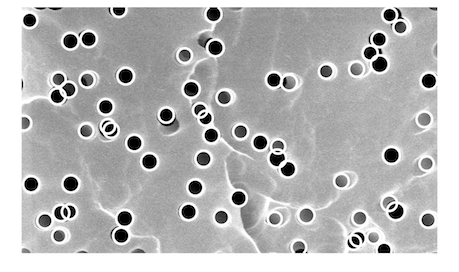
\includegraphics[scale=0.8]{Figures/115edgesWhite.png}
    \caption{Resultat einer Kreisdetektion. Gefundene Kreise sind mit einer dicken, weißen Umfangslinie an die entsprechenden Stellen gerendert worden. Mit zwei Ausnahmen wurde jedes einzelne Loch aufgespührt. Falschdetektionen (false positives) traten nicht auf.}
    \label{fig:edgesWhite}
\end{figure}

\section{Kantendetektion}
\label{ch:kantendetektion}
Die stärksten Kanten in den von uns betrachteten REM-Bildern sind diejenigen, welche die Einschusslöcher der Templatfolie umreißen. Somit liegt es nahe, dass man mit wenig Rechenaufwand eine gezielte Kantedetektion durchführen kann, um jene Kanten zu extrahieren und anhand dieser die aufgespannten Mantelflächen berechnet. 
Probleme können falsch positiv detektierte Kanten verursachen, wenn nicht orthogonal geschossene Löcher untersucht werden. Hier kann unter Umständen der Fall eintreten, dass unvollständige Kreise oder Verschmierungen (siehe Abb. \ref{fig:remScharf1Edge}) zutage treten, welche eine präzise Umrissabschätzung erschweren.

\paragraph{Grundlegender Algorithmus zur Detektion von Kanten}
\begin{enumerate}
\item Weichzeichnung des Bildes zur Herausfilterung von Rauschen
\item Berechnung des Gradientenbildes
\item Anwendung einer Schwellenwertoperation, um signifikante Gradienten zu finden
\item "Ausdünnung" von Kanten, um Konturen mit einer Dicke von einem Pixel zu erhalten und damit eine genaue Lokalisation zu ermöglichen
\item Optional: Diese Kantenpixel miteinander verbinden, um eine durchgehende Kontur zu erhalten
\end{enumerate}

\subsection{Canny Algorithmus}
Wie bereits im Einführungskapitel beschrieben, wird aufgrund seiner hervorragenden Performance der Canny-Filter für diese Aufgabe auserwählt. Er wird im Folgenden nur grob beschrieben, da auch hier eine fertige Implementierung seitens \textsc{Matlab} verwendet wird.\\
Der Canny-Filter arbeitet mit der zweiten Ableitung und nimmt zusätzlich die Positionen der Nulldurchgänge der zweiten Ableitung als Kantenposition hinzu. Um die Anfälligkeit gegenüber Rauschen zu mindern, wird ein geeigneter Glättungsfilter, wie beispielsweise der Laplacian-of-Gaussian-Operator [10].\\

\paragraph{Anschaulicher Algorithmus}
\begin{enumerate}
\item Bild mit Gauss-Filter filtern: 
\item Finde Betrag und Orientierung der Kanten
\item Non-Maximum suppression: Ausdünnung von Multi-Pixel-Kanten zu 1-Pixel-Kanten (entspricht einer Breite von einem Pixel)
\item Verbindung und Schwellenwertbildung von Kantenpixeln: a) Bestimmung zweier Schwellwerte: niedrig und hoch b) Nutzung des hohen Schwellwertes, um Konturen hoher Kantenstärke zu bilden und c) die Fortführung dieser Konturen mithilfe des niedrigen Schwellwertes (Details zu diesem Vorgehen finden sich im nächsten Paragraphen zur Schwellenwert Hysterese)
\end{enumerate}

\paragraph{Canny Schwellenwert Hysterese}
Im Wesentlichen werden zur Kantenbildung vom Canny-Algorithmus folgende Arbeitsschritte durchgeführt:
\begin{enumerate}
\item Wende Kantenfilter mit hohem Schwellenwert an, um besonders ausgeprägte Kanten zu finden
\item Verbinde die gefundenen, starken Kantenpixel miteinander, um starke Konturen zu bilden
\item Wende nun Kantenfilter mit einem niedrigen Schwellenwert an, um schwache, aber plausible Kanten zu finden
\item Erweitere nun die starken Kanten in Richtung der schwachen Kantenpixel
\end{enumerate}

Ob das Ergebnis zufriedenstellend ist, lässt sich pauschal nicht vorhersagen und bedarf in der Regel einer experimentellen Versuchsreihe.\\
Da die reine Kantendetektion zur Oberflächenbestimmung in dieser Arbeit nur eine mögliche Alternative darstellt, findet eine weitergehende Vertiefung der Kantendetektion im Rahmen dieser Arbeit nicht statt. Die Kanten für die in Kapitel \ref{pixelbasierteUmfangsberechnung} vorgestellte pixelbasierte Oberflächenberechnung liefert die in \textsc{Matlab} vorimplementierte Version des Canny-Algorithmus in Quelltext \ref{lst:edge_canny}.

\begin{lstlisting}[language=MATLAB, caption=Methodensignatur der Funktion \lstinline|edge| unter Auswahl des Canny Filters, label=lst:edge_canny]
BW = edge(Image,'canny',THRESH,SIGMA);
\end{lstlisting}

Beispielhafte Kantendetektionen mithilfe vom Canny-Algorithmus können Abbildungen \ref{fig:remScharf1} und \ref{fig:remScharf2} entnommen werden.

\chapter{Umfangs- und Oberflächenberechnung}
\label{ch:umfangsberechnung}
In diesem Kapitel werden zwei Möglichkeiten der Oberflächenberechnung vorgestellt. Hierbei werden zwei wichtige Vereinfachungen für die Beschaffenheit der Nanoröhrchen getroffen:

\begin{enumerate}
\item Das Volumen eines einzelnen Röhrchens entspricht einem geometrischen Zylinder
\item Jedes Röhrchen steht orthogonal zur Grundfläche und stellt damit einen in $z$-Richtung invarianten Körper dar
\end{enumerate}

Auf diesen beiden Annahmen beruhend, kann die Mantelfläche eines einzelnen Nanoröhrchens direkt mit $2 \pi r h$ angegeben werden. Dabei entspricht $r$ dem Radius der Zylindergrundfläche und $h$  der Zylinderhöhe.
In der Praxis kann es jedoch passieren, dass sich in einem Drahtarray mehrere Röhrchen an ihrer Wurzel überschneiden und damit eine einfache Berechnung der Oberfläche mit obiger Formel nicht möglich ist. Im folgenden Abschnitt \ref{sec:geomUmfangsberechnung} wird auf die Berechnung einer durch die Überlappung mehrerer Röhren entstandenen Umfangslinie näher eingegangen. 

\section{Geometrische Umfangsberechnung}
\label{sec:geomUmfangsberechnung}
Dieser Abschnitt befasst sich mit dem mit dem mathematischen Hintergrund des geometrischen Problems der Berechnung des Umfangs von beliebig vielen, überlappenden Kreisen und dessen Lösung mithilfe eines Algorithmus am Ende des Kapitels.\\

\subsection{Überlappung zweier Kreise}
Zu Beginn soll sich die Untersuchung lediglich auf den Umfang zweier sich schneidender Kreise beziehen und erst in einem weiteren Schritt auf die Lösung des Problems von beliebig vielen Überschneidungen an beliebigen Positionen in Abschnitt \ref{subsec:beliebigeAnzahlKreise} ausgeweitet werden.

\begin{figure}[h!]
\begin{subfigure}[b]{0.475\textwidth}
\centering
\begin{tikzpicture}[
    scale=2,
    >=stealth,
    point/.style = {draw, circle,  fill = black, inner sep = 1pt},
    dot/.style   = {draw, circle,  fill = black, inner sep = .2pt},
  ]
	\coordinate (R1) at (1,1); % Mittelpunkt des ersten Kreises
	\coordinate (R2) at (2.5,1); % Mittelpunkt des zweiten Kreises
	
	% Kreismittelpunkte
	\node (M1) at (R1) [point, label = {below:$M_1$}]{};
	\node (M2) at (R2) [point, label = {below:$M_2$}]{};
	
	% Bögen
	\draw[thick] (R1) ++(41.41:1) arc (41.41:318.59:1);
	\draw[dashed] (R1) ++(-41.41:1) arc (-41.41:41.41:1);
	\draw[thick] (R2) ++(221.41:1) arc (221.41:498.59:1);
	\draw[dashed] (R2) ++(138.59:1) arc (138.59:221.41:1);
	
	\draw[->] (R1) ++(100:1.2) arc (100:160:1.2) node[midway, sloped, above]{$l$};
	
	% Radius und Abstand der Kreise einzeichnen
	\draw[semithick,gray!50!black] (R2) -- node [below right] {$r$} +(30:1cm);
	\draw[semithick,gray!50!black] (R1) -- node [below] {$d$} (R2);
\end{tikzpicture}
\caption{Zwei überschneidende Kreis und deren\\resultierende Umfangslinie}
\label{fig:zweiKreise}
\end{subfigure}
\begin{subfigure}[b]{0.475\textwidth}
\centering
\begin{tikzpicture}[
    scale=2.5,
    >=stealth,
    point/.style = {draw, circle,  fill = black, inner sep = 1pt},
    dot/.style   = {draw, circle,  fill = black, inner sep = .2pt},
  ]
    \clip (-0.1,0.6) rectangle (2,2.4);
	\coordinate (R1) at (1,1); % Mittelpunkt des ersten Kreises
	\coordinate (R2) at (2.5,1); % Mittelpunkt des zweiten Kreises
	
	% Kreismittelpunkte
	\node (M1) at (R1) [point, label = {left:$M_1$}]{};
	\node (M2) at (R2) [point, label = {below:$M_2$}]{};
	
	% Bögen
	\draw[thick] (R1) ++(41.41:1) arc (41.41:180:1);
	%\draw[dashed] (R1) ++(-41.41:1) arc (-41.41:41.41:1);
	%\draw[thick] (R2) ++(221.41:1) arc (221.41:498.59:1);
	%\draw[dashed] (R2) ++(138.59:1) arc (138.59:221.41:1);
	
	% Radius und Abstand der Kreise einzeichnen
	\draw[thick] (R1) -- node [below] {$\frac{d}{2}=r\cos(\beta)$} (1.75,1);
	\draw (R1) -- node [above] {$r$} +(41.41:1);
	\draw[dashed] (1.75,1) -- +(0,0.66);
	\filldraw[fill=white,draw=gray!50!black] (R1) -- (1.3,1)
            arc [start angle=0, end angle=41.41, radius=0.3] -- cycle;
    \draw (1.2,1.065) node[gray!50!black] {$\beta$};
	
	% Schnittpunkt des Kreises
	\node (S) at (1.75,1.66) [point, label = right:$S$] {};
	
	\draw[->] (R1) ++(70:1.2) arc (70:140:1.2) node[midway, sloped, above]{$l_1$};
	
\end{tikzpicture}
\caption{Zusammenhang zwischen Winkel $\beta$ und dem Abstand $d$ beider Kreismittelpunkte}
\label{fig:winkelBerechnung}
\end{subfigure}
\caption{Weitere Größen und deren Orientierung im Raum}
\end{figure}

\paragraph{Problemstellung}
Gegeben seien zwei Kreise mit dem Radius $r$, deren Mittelpunkte $M_1$ und $M_2$ sich im Abstand $d$ zueinander befinden. Dabei sollen diese auf ihren gemeinsamen Umfang $l$ untersucht werden. Wird $d < 2r$ gewählt, so findet eine Überschneidung statt. Dadurch reduziert sich der Gesamtumfang im Vergleich zu zwei Einzelkreisen (gestrichelte Linie in Abb. \ref{fig:zweiKreise}).

\paragraph{Mathematische Herleitung}
Für die Berechnung des zum Umfang beitragenden Bogenstücks wird der Winkel $\beta$, 
definiert, dessen Schenkel die Strecken $\overline{M_1M_2}$ und $\overline{M_1S}$ bilden. 
$S$ ist hierbei einer der Schnittpunkte der überlappenden Kreise. Dabei gilt gemäß Abbildung \ref{fig:winkelBerechnung} folgender Zusammenhang:

\begin{equation}
\beta = \cos^{-1}\left(\frac{d}{2r}\right)
\label{eq:beta}
\end{equation}

Mit dem berechneten Winkel $\beta$ kann nun der Teil des Kreisbogens bestimmt werden, der nach der Überschneidung übrig bleibt. Dazu wird die Bogenlänge des verbleibenden Kreissegments $l_1$ berechnet, wie es folgende Gleichung zeigt: \\
\begin{equation}
\begin{split}
l_1 &= 2 \pi r\left(1-\frac{\beta}{\pi}\right) \\
    &= 2 \pi r\left(1-\frac{\cos^{-1}\left(\frac{d}{2r}\right)}{\pi}\right)
\end{split}
\label{eq:einBogenteil}
\end{equation}

Weiterhin gilt für den Gesamtumfang die resultierende Umfangslinie $l$:
\begin{equation}
l = 2 l_1 = 4 \pi r\left(1-\frac{\cos^{-1}\left(\frac{d}{2r}\right)}{\pi}\right). \\
\label{eq:beideBogenteile}
\end{equation}

Aufgrund der Spiegelsymmetrie gelten die gleichen Zusammenhänge auch für den Kreis $C_2$ um den Mittelpunkt $M_2$ und münden in Gleichung \ref{eq:beideBogenteile}

\subsection{Überlappung beliebiger Anzahl Kreise}
\label{subsec:beliebigeAnzahlKreise} 

Gegeben sei dabei eine beliebige Anordung von $n$ Kreisen $C_1, C_2,...,C_n$ mit den Mittelpunkten $M_1, M_2,...,M_n$. Eine beispielhafte Anordnung solcher Kreise kann Abbildung \ref{img:5Kreise} entnommen werden.\\ 

\begin{figure}[h!]
\centering
\begin{tikzpicture}[
    scale=1.5,
    >=stealth,
    point/.style = {draw, circle,  fill = black, inner sep = 1pt},
    dot/.style   = {draw, circle,  fill = black, inner sep = .2pt},
  ]
  
	\coordinate (R1) at (3.2,4); % Mittelpunkt des ersten Kreises
	\coordinate (R2) at (1.6,3.6); % Mittelpunkt des zweiten Kreises
	\coordinate (R3) at (4.2,4.4); % Mittelpunkt des dritten Kreises
	\coordinate (R4) at (4.6,3); % Mittelpunkt des vierten Kreises
	\coordinate (R5) at (2,6); % Mittelpunkt des fünften Kreises
	
	% Kreismittelpunkte
	\node (M1) at (R1) [point, label = {below:$M_1$}]{};
	\node (M2) at (R2) [point, label = {below:$M_2$}]{};
	\node (M3) at (R3) [point, label = {right:$M_3$}]{};
	\node (M4) at (R4) [point, label = {below:$M_4$}]{};
	\node (M5) at (R5) [point, label = {below:$M_5$}]{};
	
	% Bögen
	% C1
	\draw[thick] (R1) ++(79.22:1) arc (79.22:159.59:1);
	\draw[thick] (R1) ++(228.49:1) arc (228.49:293.81:1) node[midway, below]{$C_1$};
	\draw[dashed] (R1) ++(159.59:1) arc (159.59:228.49:1);
	\draw[dashed] (R1) ++(293.81:1) arc (293.81:439.22:1);
	
	% C2
	\draw[thick] (R2) ++(48.49:1) arc (48.49:339.59:1) node[midway, left]{$C_2$};
	\draw[dashed] (R2) ++(339.59:1) arc (339.59:408.49:1);
	
	% C3
	\draw[thick] (R3) ++(329.23:1) arc (329.23:504.38:1) node[midway, above right]{$C_3$};
	\draw[dashed] (R3) ++(144.38:1) arc (144.38:329.23:1);
	
	% C4
	\draw[thick] (R4) ++(175.12:1) arc (175.12:422.67:1) node[midway, below right]{$C_5$};
	\draw[dashed] (R4) ++(62.67:1) arc (62.67:175.12:1);
	
	% C5
	\draw[thick] (R5) ++(0:1) arc (0:360:1) node[midway, left]{$C_5$};
	
\end{tikzpicture}
\caption{Beispielhafte Anordnung mehrerer Kreise}
\label{img:5Kreise}
\end{figure}

Zu beachten ist hier der resultierende Umfang der Anordnung (durchgezogene, dicke Linie). Diesen gilt es im Folgenden schrittweise zu berechnen.

\subsubsection{Definitionen und mathematische Zusammenhänge}
Der am Ende dieses Abschnitts vorgestellte Algorithmus bestimmt in Form von Adjazenzmatrizen die paarweisen Abstände, Abstandsvektoren und Schnittpunkte aller Kreise zueinander. Anhand der Orientierung und Lage dieser Größen kann über Vergleichsoperationen der nicht überdeckte Teil des Bogens jedes einzelnen Kreises bestimmt werden. Dieser wird zur letztendlichen Berechnung der Oberfläche herangezogen. Veranschaulicht wird die Bestimmung der verbleibenden Kreisbogensegmente durch ein sogenanntes Spurendiagramm (Abb. \ref{fig:schritt1}).

\paragraph{Berechnung der Abstandsvektoren und deren Orientierung}
Fasst man die Kreismittelpunkte als Knoten und die Abstandsvektoren als Gewichte der Kanten auf, kann zu jeder beliegen Kreiskonfiguration eine Adjazenzmatrix aufgestellt werden, welche alle benötigten Größen in kompakter Form speichern kann. In einem weiteren Schritt können aus dieser Adjazenzmatrix die exakten Schnittpunkte der Kreise ermittelt und zur Berechnung der nicht überdeckten Kreisbogen herangezogen werden.\\
Die Abstandsvektoren werden in einer Adjazenzmatrix $D = \left[ \vec{d_{ij}} \right]$ durch ihre Einträge definiert als [Quellenverweis]\\
\begin{equation} 
\vec{d_{ij}} = 
\begin{cases} 
      \vec{m_j} - \vec{m_i} 	& \text{falls} \; i \neq j \\
      0						& \text{sonst}.
\end{cases}
\end{equation}

Hierbei ist $\vec{d_{ij}}$ der Abstandsvektor von Raumpunkt $M_i$ des Kreises $C_i$ zum Raumpunkt $M_j$ des Kreises $C_j$. Die Vektoren $\vec{m_i}$ und $\vec{m_j}$ stellen dabei die Ortsvektoren der Kreismittelpunkte dar.\\

Darauf aufbauend wird nun für jeden Kreis eine Orientierung der von ihm ausgehenden Abstandsvektoren definiert. Die Orientierung eines Abstandsvektors wird dabei wie in Abbildung \ref{fig:distanzVektorLage} in einem in Gleichung \ref{eq:schnittwinkel} definierten Winkel $\alpha_{ij}$ gespeichert. Wir fassen diesen Winkel als denjenigen auf, der von $\vec{e_x}$ (welche der gestrichelten Horizontalen durch den Punkt $M_1$ entspricht) und dem Distanzvektor $\vec{d_{ij}}$ aufgespannt wird. Er verläuft im mathematisch positiven Sinn beginnend von der $x$-Achse eines kartesischen Koordinatensystems, dessen Ursprung genau im Mittelpunkt $M_i$ des betreffenden Kreises $C_i$ liegt, vom ersten bis zum vierten Quadranten.\\

\begin{figure}[h!]
\begin{subfigure}[b]{0.5\textwidth}
\centering
\begin{tikzpicture}[
    scale=2,
    >=stealth,
    point/.style = {draw, circle,  fill = black, inner sep = 1pt},
    dot/.style   = {draw, circle,  fill = black, inner sep = .2pt},
  ]
  
	\coordinate (R1) at (1,1); % Mittelpunkt des ersten Kreises
	\coordinate (R2) at (1.8,2.4); % Mittelpunkt des zweiten Kreises
	
	% Kreismittelpunkte
	\node (M1) at (R1) [point, label = {below left:$M_1$}]{};
	\node (M2) at (R2) [point, label = {above right:$M_2$}]{};
	
	% Bögen
	% C1
	\draw[thick] (R1) ++(96.53:1) arc (96.53:383.98:1);
	\draw[dashed] (R1) ++(23.98:1) arc (23.98:96.53:1);
	
	% C2
	\draw[thick] (R2) ++(276.53:1) arc (276.53:563.98:1);
	\draw[dashed] (R2) ++(203.98:1) arc (203.98:276.53:1);
	
	%\draw[->] (R1) ++(100:1.2) arc (100:160:1.2) node[midway, sloped, above]{$l$};
	
	% Abstandsvektor d12
	\draw[thick,->] (R1) -- (R2);
	\node at (1.4,2.15) {$\vec{d_{12}}$};
	
	% Hilfslinie zur Sichtbarmachung der 0°/360° Grenze
	\draw[dashed] (R1) -- (2.7,1);
	\node [below] at (1.5,1) {$\alpha = \ang{360}$};
	\node [above] at (1.5,1) {$\alpha = \ang{0}$};
	
	% Winkelpfeil
	\draw[->] (R1) ++(0:1.2) arc (0:60.26:1.2) node[midway, sloped, above]{$\alpha_{12}$};
	
\end{tikzpicture}
\caption{Orientierung eines Abstandsvektors}
\label{fig:distanzVektorLage}
\end{subfigure}
\begin{subfigure}[b]{0.5\textwidth}
\centering
\begin{tikzpicture}[
    scale=3,
    >=stealth,
    point/.style = {draw, circle,  fill = black, inner sep = 1pt},
    dot/.style   = {draw, circle,  fill = black, inner sep = .2pt},
  ]
  	\clip (0.5,0.7) rectangle (2.25,2.6);
	\coordinate (R1) at (1,1); % Mittelpunkt des ersten Kreises
	\coordinate (R2) at (1.8,2.4); % Mittelpunkt des zweiten Kreises
	
	% Kreismittelpunkte
	\node (M1) at (R1) [point, label = {below left:$M_1$}]{};
	\node (M2) at (R2) [point, label = {above right:$M_2$}]{};
	
	% Bögen
	% C1
	\draw[thick] (R1) ++(96.53:1) arc (96.53:383.98:1);
	\draw[dashed] (R1) ++(23.98:1) arc (23.98:96.53:1);
	
	% C2
	\draw[thick] (R2) ++(276.53:1) arc (276.53:563.98:1);
	\draw[dashed] (R2) ++(203.98:1) arc (203.98:276.53:1);
		
	% Abstandsvektor d12
	\draw[thick,->,gray!50] (R1) -- (R2);
	\node[gray!50] at (1.4,2.15) {$\vec{d_{12}}$};
	
	% Kennzeichnung der Schnittpunkte
	\node (S12a) at ($ (R1) + (96.53:1) $) [point, label = {[label distance=0.2cm]176:$S_{12}^{(1)}$}]{};
	\node (S12b) at ($ (R1) + (23.98:1) $) [point, label = {[label distance=0.2cm]350:$S_{12}^{(2)}$}]{};
	
	% Vektoren zu den Schnittpunkten
	% Vektor M1->S12(1)
	\draw[thick,->] (R1) -- (S12a);
	% Vektor M1->S12(2)
	\draw[thick,->] (R1) -- (S12b);
	
	% y-Einheitsvektor
	\draw[thick,->] (R1) -- (1.2,1) node[below, midway]{$\vec{e_x}$};
	
	% Hilfslinie zur Sichtbarmachung der 0°/360° Grenze
	\draw[dotted] (R1) -- (2.7,1);
	
	% Winkelpfeile
	\draw[->] (R1) ++(0:0.4) arc (0:96.53:0.4) node[midway, sloped, above]{$\gamma_{12}^{(1)}$};
	\draw[->] (R1) ++(0:0.6) arc (0:23.98:0.6) node[midway, sloped, above]{$\gamma_{12}^{(2)}$};
	\draw[->] (R1) ++(60.26:0.75) arc (60.26:96.53:0.75) node[midway, sloped, above]{$\beta_{12}$};
	
\end{tikzpicture}
\caption{Kreis-Schnittpunkte und ihre Lage}
\label{fig:schnittWinkelLage}
\end{subfigure}
\caption{Weitere Größen und deren Orientierung im Raum}
\end{figure}

Um den definierten Winkel $\alpha_{ij}$ zu erhalten, wird eine Schnittwinkel-Berechnung [11] gemäß Gleichung \ref{eq:schnittwinkel}  des jeweiligen Distanzvektors $d_{ij}$ und des $\vec{e_x}$-Einheitsvektors durchgeführt.

\begin{equation} 
\alpha_{ij} := \angle(\vec{d_{ij}},\vec{e_x}) = \cos^{-1}{\frac{\abs{\vec{d_{ij}}\cdot\vec{e_x}}}{\abs{\vec{d_{ij}}}\cdot\abs{\vec{e_x}}}}
\label{eq:schnittwinkel}
\end{equation}

Dabei wird eine weitere, symmetrische  Adjazenzmatrix $D_\alpha = \left[ \alpha_{ij} \right] $ definiert, welche in analoger Indizierung die Orientierung der Abstandsvektoren speichert. Wünschenswert ist hierbei ein Wertebereich von $[0,360]$ für den Winkel $\alpha_{ij}$. Allerdings stellt die Schnittwinkelformel \ref{eq:schnittwinkel} nur einen Bereich von $[0,180]$ zur Verfügung, so dass Gleichung  \ref{eq:schnittwinkel} zu folgender Form erweitert werden muss:\\

\begin{equation} 
\alpha_{ij} = \begin{cases} 
      \cos^{-1}{\frac{\abs{\vec{d_{ij}}\cdot\vec{e_x}}}{\abs{\vec{d_{ij}}}\cdot\abs{\vec{e_x}}}} & \vec{d_{ij,y}}\geq 0 \\
      \ang{360} - \cos^{-1}{\frac{\abs{\vec{d_{ij}}\cdot\vec{e_x}}}{\abs{\vec{d_{ij}}}\cdot\abs{\vec{e_x}}}} & \vec{d_{ij,y}} < 0 \\
   \end{cases}
\label{eq:schnittWinkelBereichserweiterung}
\end{equation}
Ist die $y$-Komponente des Distanzvektors $\vec{d_{ij}}$ kleiner Null, so liegt ein Vektor mit negativer Steigung vor und dem damit verbundenen überstumpfen Winkel $\alpha$. Da \ref{eq:schnittwinkel} in diesem Fall den spitzen Winkel beider Schnittgeraden berechnet, muss dieser von $\ang{360}$ subtrahiert werden, um den gewünschten Winkel $a_{ij}$ zu erhalten.

\paragraph{Lage der Schnittpunkte}
Mithilfe der Lage der Abstandsvektoren lassen sich nun ebenfalls auch die Orientierungen der Schnittpunkte $S_{ij}$ festhalten. Die genauen Positionen der Schnittpunkte des Kreises $C_i$ mit dem Kreis $C_j$ können dabei beispielhaft Abbildung \ref{fig:schnittWinkelLage} entnommen werden. \\
Mit Gleichung \ref{eq:beta} kann der Winkel $\beta_{ij}$ mit 
\begin{equation}
\beta_{ij} = \cos^{-1}\frac{\abs{\vec{d_{ij}}}}{2r}
\end{equation}
direkt angegeben werden.\\

Weiterhin ist zu beachten, dass sich schneidende Kreise stets zwei Schnittpunkte miteinander haben. Aus diesem Grund wird für jedes überlappende Kreispaar in Gleichung \ref{eq:bogenkomponenten} ein Bogen $b_{ij}$ definiert, welcher den Anfangs- und Endwert des nicht verdeckten Kreisbogens als abgeschlossenes Intervall $[\gamma_{ij}^{(1)}, \gamma_{ij}^{(2)}]$ speichert. Die Grenzen dieser Menge entsprechen dabei gerade den Winkeln, an denen sich die Schnittpunkte schneidenden Kreise befinden. Über den Modulo-Operator wird sichergestellt, dass Unter- und Überschreitungen des gültigen Winkelbereichs $[0,360]$ auf den korrekten Wert abgebildet werden. 

\begin{equation} 
b_{ij} := \left[ {\gamma _{ij}^{(1)},\gamma_{ij}^{(2)}} \right] 
=\left[{ (\alpha_{ij} + \beta_{ij}) \Mod{360}, (\alpha_{ij} - \beta_{ij}) \Mod{360} }\right] 
\label{eq:bogenkomponenten}
\end{equation}

Alle Intervalle $b_{ij}$ werden wiederum in einer neuen Adjazenzmatrix $A = \left[ b_{ij} \right] $ gespeichert, deren Spalte $i$ dabei als eine Menge $c_i$ von abgeschlossenenen Intervallen  aller Bögen auf dem Kreis $C_i$ gilt. In Gleichung \ref{eq:defBogenMenge} wird der Begriff einer Intervallmenge näher definiert, um im kommenden Abschnitt eine mathematische Schnittmenge mehrerer Bögen bzw. Intervalle bilden zu können. \\
\begin{equation} 
\begin{aligned}
c_i &= \left\{b_1, b_2,..., b_k\right\} \\
& = \left\{\left[\gamma_1^{(1)},\gamma_1^{(2)}\right], \left[\gamma_2^{(1)},\gamma_2^{(2)}\right],..., \left[\gamma_k^{(1)},\gamma_k^{(2)}\right]\right\}, \quad \gamma \in [0,360)
\end{aligned}
\label{eq:defBogenMenge}
\end{equation}

In Abbildung \ref{fig:dreiKreise} ist zu sehen, dass der Schnittpunkt $S_{ij}^{(1)}$, dessen Position über den Winkel $\gamma_{12}^{(1)}$ angegeben ist, der ersten Begrenzung des Intervalls $a_{12}$ entspricht. Dieser Logik folgend wird dieses Intervall über den zweiten Schnittpunkt $S_{12}^{(2)}$ und den Winkel $\gamma_{12}^{(2)}$ geschlossen. Auf diese Weise können wir aus jedem Distanzvektor ein Schnittpunkt-Paar ermitteln, deren zugehörigen Winkel die Begrenzungen eines Intervalls bilden.\\

\emph{Anmerkung:} Zu beachten ist die Möglichkeit, dass die Intervallgrenzen des Bogens $a_{ij}$ auch den Übergang des Winkels von $\ang{0}$ zu $\ang{360}$ beinhalten und damit der Endpunkt $\gamma _{ij}^{(2)}$ nominell kleiner sein kann als der Startpunkt $\gamma _{ij}^{(1)}$. Beispielsweise ist $b_{12} = [270,30]$ ein gültiger Bogenintervall.\\
In der Implementierung muss dieser Umstand in einem gesonderten Fall berücksichtigt werden.

\paragraph{Zusammenlegung von Bögen}
Sobald alle paarweisen überlappten und nicht überlappten Bogensegmente in Form von Intervallen auf den Kreisen bestimmt und in der Matrix $A$ gespeichert sind, kann die Zusammenführung dieser spaltenweise im Sinne des dazugehörigen Kreises durchgeführt werden. \\
%% Bild von drei Kreisen, um zu demonstrieren, wie sich zwei valide Bogenstücken zusammenfügen
\begin{figure}[h!]
\centering
\begin{tikzpicture}[
    scale=2,
    >=stealth,
    point/.style = {draw, circle,  fill = black, inner sep = 1pt},
    dot/.style   = {draw, circle,  fill = black, inner sep = .2pt},
  ]
  
	\coordinate (R1) at (1,1); % Mittelpunkt des ersten Kreises
	\coordinate (R2) at (1.8,2.4); % Mittelpunkt des zweiten Kreises
	\coordinate (R3) at (2.4,0.8); % Mittelpunkt des dritten Kreises 
	
	% Kreismittelpunkte
	\node (M1) at (R1) [point, label = {below left:$M_1$}]{};
	\node (M2) at (R2) [point, label = {above right:$M_2$}]{};
	\node (M3) at (R3) [point, label = {right:$M_3$}]{};
	
	% Bögen
	% C1
	\draw[thick] (R1) ++(96.53:1) arc (96.53:306.87:1) node[midway,left]{$C_1$};
	\draw[dashed] (R1) ++(306.87:1) arc (306.87:456.53:1);
	
	% C2
	\draw[thick] (R2) ++(321.86:1) arc (321.86:563.98:1) node[midway,above]{$C_2$};
	\draw[dashed] (R2) ++(203.98:1) arc (203.98:321.86:1);
	
	% C3
	\draw[thick] (R3) ++(216.87:1) arc (216.87:439.25:1) node[midway,right]{$C_3$};
	\draw[dashed] (R3) ++(79.25:1) arc (79.25:216.87:1);
	
	%\draw[->] (R1) ++(100:1.2) arc (100:160:1.2) node[midway, sloped, above]{$l$};
	
	% Hilfslinie zur Sichtbarmachung der 0°/360° Grenze
	\draw[dotted] (R1) -- (2,1);
	
	% Abstandsvektor d12
	\draw[thick,->,gray!50] (R1) -- (R2);
	\node[gray!50] at (1.4,2.15) {$\vec{d_{12}}$};
	
	% Abstandsvektor d13
	\draw[thick,->,gray!50] (R1) -- (R3) node[sloped, below left]{$\vec{d_{13}}$};
	%\node at (1.4,2.15) {$\vec{d_{12}}$};
	
	% Kennzeichnung der Schnittpunkte
	\node (S12a) at ($ (R1) + (96.53:1) $) [point, label = {[label distance=0.2cm]176:$S_{12}^{(1)}$}]{};
	\node[gray!50] (S12b) at ($ (R1) + (23.98:1) $) [point, gray!50, label = {[gray!50,label distance=0.1cm]350:$S_{12}^{(2)}$}]{};
	\node[gray!50] (S13a) at ($ (R1) + (36.87:1) $) [point, gray!50, label = {[gray!50,label distance=0.15cm]90:$S_{13}^{(1)}$}]{};
	\node (S13b) at ($ (R1) + (306.87:1) $) [point, label = {[label distance=0.2cm]0:$S_{13}^{(2)}$}]{};
	
	% Vektoren zu den Schnittpunkten
	% Vektor M1->S12(1)
	\draw[thick,->] (R1) -- (S12a);
	% Vektor M1->S12(2)
	\draw[thick,->] (R1) -- (S13b);
	
	% Winkelpfeile
	\draw[->] (R1) ++(0:0.5) arc (0:96.53:0.5) node[midway, sloped, below]{$\hat{\gamma}_{1}^{(1)}$};
	\draw[->] (R1) ++(0:0.75) arc (0:306.87:0.75) node[midway, sloped, below]{$\hat{\gamma}_{1}^{(2)}$};
	
\end{tikzpicture}
\caption{Zusammenführung der Bögen $\overline{S_{12}^{(1)}S_{12}^{(2)}}$ und $\overline{S_{13}^{(1)}S_{13}^{(2)}}$ auf Kreis $C_1$ (durchgezogene als auch gestrichelte Linien bilden gemeinsam einen Bogen)}
\label{fig:dreiKreise}
\end{figure}

Für jeden Kreis liegen nun in der Matrix $A$ diejenigen Bögen vor, die nach der Überschneidung mit jedem Nachbarkreis übrig bleiben. Der auf $C_1$ verlaufende Kreisbogen des Kreispaares $(C_1,C_2)$, welcher von $S_{12}^{(1)}$ nach $S_{12}^{(2)}$ verläuft, bildet mit dem Kreisbogen des Kreispaares $(C_1,C_3)$ eine Schnittmenge und bildet einen neuen auf $C_1$ verlaufenden Kreisbogen, welcher von $S_{12}^{(1)}$ nach $S_{13}^{(2)}$ verläuft. Abbildung \ref{fig:dreiKreise} verdeutlicht diesen Sachverhalt.\\
Da jeder Kreis nach dieser Prozedur eine unterschiedliche Anzahl an nicht überlappten Bogensegmenten besitzt, beinhaltet nach Definition \ref{eq:neueIntervallMenge} jede neue Intervallmenge $\hat{c}_i$ eine individuelle Anzahl $l$ an Intervallen. 
\begin{equation}
\begin{aligned}
\hat{c}_i &= b_1 \cap b_2 \cap ... \cap b_k, \quad b_i \in c_i \\
&= \left\{\hat{b}_1, \hat{b}_2,..., \hat{b}_l\right\} \\
& = \left\{\left[\hat{\gamma}_1^{(1)},\hat{\gamma}_1^{(2)}\right], \left[\hat{\gamma}_2^{(1)},\hat{\gamma}_2^{(2)}\right],..., \left[\hat{\gamma}_l^{(1)},\hat{\gamma}_l^{(2)}\right]\right\}, \quad \hat{\gamma} \in [0,360)
\end{aligned}
\label{eq:neueIntervallMenge}
\end{equation}
Die schrittweise Berechnung dieser Schnittmenge wird in Algorithmus \ref{alg:arcMerging} beschrieben. Nach dessen Anwendung auf die Bogenintervalle $b_i$ jeden Kreises, gibt dieser die neuen Bogenintervalle $\hat{b}_i$ innerhalb der Menge $\hat{c}_i$ als Prozedurausgabe \textit{MergedArcsOnCirlce} aus und speichert sie in einer neuen Liste zur weiteren Verarbeitung.\\

\begin{algorithm}[t]
  \caption{Schnittmengenbildung aller Bögen eines Kreises}
  \label{alg:arcMerging}
  \begin{algorithmic}[1]
    \Procedure{MergeArcsForCircle}{$\textit{circle}$}%\Comment{The g.c.d. of a and b}
    \State \textsc{Step 1 – collect start and end points of all arcs}
    \State Create an empty list $\textit{StartPointsOnCircle} \gets \{\}$
	\State Create an empty list $\textit{EndPointsOnCircle} \gets \{\}$
	\For{all arcs $(\gamma^{(1)}, \gamma^{(2)})$ in \textit{circle}}
		\State Add $\gamma^{(1)}$ to \textit{StartPointsOnCircle}
		\State Add $\gamma^{(2)}$ to \textit{EndPointsOnCircle}
	\EndFor
	\State Sort \textit{StartPointsOnCircle} and \textit{EndPointsOnCircle} by ascending order
	\State Remove duplicates in \textit{StartPointsOnCircle} and \textit{EndPointsOnCircle}
	\\
	\State \textsc{Step 2 – remove start and end points which are located in overlapped areas}
	\For{all arcs $(\gamma^{(1)}, \gamma^{(2)})$ in \textit{circle}}
		\If{$\gamma^{(2)} - \gamma^{(1)} > 0$} %\Comment{Arc range consists of one segment}
			\State Delete all values $s_i$ from \textit{StartPointsOnCircle} if $s_i < \gamma^{(1)}$ \textbf{or} $s_i > \gamma^{(2)}$
			\State Delete all values $e_i$ from \textit{EndPointsOnCircle} if $e_i < 				\gamma^{(1)}$ \textbf{or} $e_i > \gamma^{(2)}$
		\Else %\Comment{Arc range consists of two segments}
			\State Delete all values $s_i$ from \textit{StartPointsOnCircle} if $s_i < 				\gamma^{(1)}$ \textbf{and} $s_i > \gamma^{(2)}$
			\State Delete all values $e_i$ from \textit{EndPointsOnCircle} if $e_i < 				\gamma^{(1)}$ \textbf{and} $e_i > \gamma^{(2)}$
		\EndIf
	\EndFor
	\\
	\State \textsc{Step 3 – stitch start and end points in the right way together}
	\State Create an empty list $\textit{MergedArcsOnCircle} \gets \{\}$
	\State Set up a counter $k \gets 1$ 
	\For{all values $\gamma^{(1)}$ in \textit{StartPointsOnCircle}}
		\State Iterate over \textit{EndPointsOnCircle},
			   find first value $e$ which meets $e > \gamma^{(1)}$
		\If{$e \neq 0$}
			\State Create arc $\hat{b}_i = (\hat{\gamma}_i^{(1)},\hat{\gamma}_i^{(2)}) \gets (\gamma^{(1)},e)$
			\State \textit{MergedArcsOnCircle}$(k) \gets \hat{b}_i$
			\State Increment $k$
		\Else
			\State Create arc $\hat{b}_i = (\hat{\gamma}_i^{(1)},\hat{\gamma}_i^{(2)}) \gets (\gamma^{(1)},$\textit{EndPointsOnCircle}$(1))$
			\State \textit{MergedArcsOnCircle}$(k) \gets \hat{b}_i$
		\EndIf
	\EndFor
	\State \textbf{return} $\textit{MergedArcsOnCircle}$
    \EndProcedure
  \end{algorithmic}
\end{algorithm}

Abbildung \ref{fig:schritte1-4} stellt den Zusammenhang zwischen den obigen mathematischen Definitionen und dem Algorithmus \ref{alg:arcMerging} her und zeigt die schrittweise Ausführung exemplarisch am Kreis $C_1$ aus Abbildung \ref{img:5Kreise}.\\

%% BEGINN DER 2x2 ABBILDUNG ZUR VERANSCHAULICHUNG DER DREI STEPS DES ALGORITHMUS
\begin{figure}
        \centering
        \begin{subfigure}[b]{0.475\textwidth}
        		\centering
			\begin{tikzpicture}
	\begin{axis}[width=8cm,xlabel={$\gamma$ (\textdegree)}, xtick={0,90,180,270,360}, xmin=0, xmax=360, ytick={1,...,4}, yticklabels={$b_{15}$,$b_{14}$,$b_{13}$,$b_{12}$},xmajorgrids]
	% Bogenspuren mit Kreis C_2
	\addplot[mark=*] plot coordinates  { (228.49,4) (370,4) } node[below, pos=0] {$\gamma^{(1)}_{12}$} ;
	\addplot[mark=*] plot coordinates { (-10,4) (159.59,4) } node[below, pos=1] {$\gamma^{(2)}_{12}$};
	
	% Bogenspuren mit Kreis C_3
	\addplot[mark=*] plot coordinates { (79.22,3) (324.38,3) } node[below, pos=0] {$\gamma^{(1)}_{13}$} node[below, pos=1] {$\gamma^{(2)}_{13}$};
	
	% Bogenspuren mit Kreis C_4
	\addplot[mark=*] plot coordinates { (355.12,2) (370,2) } node[below, pos=-.7] {$\gamma^{(1)}_{14}$};
	\addplot[mark=*] plot coordinates { (-10,2) (293.81,2) } node[below, pos=1] {$\gamma^{(2)}_{14}$};
	
	% Bogenspuren mit Kreis C_5
	\addplot[mark=*] plot coordinates { (0,1) (360,1) } node[above, pos=0.05] {$\gamma^{(1)}_{15}$} node[above, pos=0.957] {$\gamma^{(2)}_{15}$};
	
	% Füge noch eine graue Box zur Kennzeichnung der übriggebliebenen Bogenstücken hinzu
%	\fill [gray!60,fill opacity=0.2] (axis cs:79.22,1) rectangle (axis cs:159.59,4);
%	\fill [gray!60,fill opacity=0.2] (axis cs:228.49,1) rectangle (axis cs:293.81,4);
	\end{axis}
\end{tikzpicture}
            \caption{Schritt 1: Start- und Endpunkte der Bögen $a_{ij}$ sammeln}  
            \label{fig:schritt1}
        \end{subfigure}
        \hfill
        \begin{subfigure}[b]{0.475\textwidth}  
            \centering 
            \begin{tikzpicture}
	\begin{axis}[width=8cm,xlabel={$\gamma$ (\textdegree)}, xtick={0,90,180,270,360}, xmin=0, xmax=360, ytick={1,...,4}, yticklabels={$b_{15}$,$b_{14}$,$b_{13}$,$b_{12}$},xmajorgrids]
	% Bogenspuren mit Kreis C_2
	\addplot[mark=*] plot coordinates  { (228.49,4) (370,4) } node[below, pos=0] {$\gamma^{(1)}_{12}$} ;
	\addplot[mark=*] plot coordinates { (-10,4) (159.59,4) } node[below, pos=1] {$\gamma^{(2)}_{12}$};
	
	% Bogenspuren mit Kreis C_3
	\addplot[mark=*] plot coordinates { (79.22,3) (324.38,3) } node[below, pos=0] {$\gamma^{(1)}_{13}$} node[cross, below, pos=1] {$\gamma^{(2)}_{13}$};
	
	% Bogenspuren mit Kreis C_4
	\addplot[mark=*] plot coordinates { (355.12,2) (370,2) } node[cross, below, pos=-.7] {$\gamma^{(1)}_{14}$};
	\addplot[mark=*] plot coordinates { (-10,2) (293.81,2) } node[below, pos=1] {$\gamma^{(2)}_{14}$};
	
	% Bogenspuren mit Kreis C_5
	\addplot[mark=*] plot coordinates { (0,1) (360,1) } node[cross, above, pos=0.05] {$\gamma^{(1)}_{15}$} node[cross, above, pos=0.957] {$\gamma^{(2)}_{15}$};
	
	% Füge noch eine graue Box zur Kennzeichnung der übriggebliebenen Bogenstücken hinzu
	\fill [gray!60,fill opacity=0.2] (axis cs:79.22,0) rectangle (axis cs:159.59,5);
	\fill [gray!60,fill opacity=0.2] (axis cs:228.49,0) rectangle (axis cs:293.81,5);
	\end{axis}
\end{tikzpicture}
            \caption{Schritt 2: Entferne Start- und Endpunkte aus überdeckten Bereichen}   
            \label{fig:schritt2}
        \end{subfigure}
        \vskip\baselineskip
        \begin{subfigure}[b]{0.475\textwidth}   
            \centering 
            \begin{tikzpicture}
	\begin{axis}[height=3.5cm, width=8cm,xlabel={$\hat{\gamma}$ (\textdegree)}, xtick={0,90,180,270,360}, xmin=0, xmax=360, ytick={1}, yticklabels={$\hat{c}_1$},xmajorgrids]
	% Bogenspuren mit Kreis C_2
	\addplot[mark=*] plot coordinates  { (79.22,1) (159.59,1) } node[below, pos=0] {$\hat{\gamma}^{(1)}_{1}$} node[below, pos=1] {$\hat{\gamma}^{(2)}_{1}$};
	\draw[decoration={brace,raise=5pt,amplitude=3pt},decorate]
  (79.22,0) -- node[above=6pt] {$\hat{b}_{1}$} (159.59,0);
	\addplot[mark=*] plot coordinates { (228.49,1) (293.81,1) } node[below, pos=1] {$\hat{\gamma}^{(2)}_{2}$} node[below, pos=0] {$\hat{\gamma}^{(1)}_{2}$};
	\draw[decoration={brace,raise=5pt,amplitude=3pt},decorate]
  (228.49,0) -- node[above=6pt] {$\hat{b}_{2}$} (293.81,0);
	% Füge noch eine graue Box zur Kennzeichnung der übriggebliebenen Bogenstücken hinzu
	\fill [gray!60,fill opacity=0.2] (axis cs:79.22,0) rectangle (axis cs:159.59,2);
	\fill [gray!60,fill opacity=0.2] (axis cs:228.49,0) rectangle (axis cs:293.81,2);
	\end{axis}	
\end{tikzpicture}
            \caption{Schritt 3: Setze übriggebliebene Punkte zu neuen Bögen $\hat{b}_1$ und $\hat{b}_2$ zusammen}  
            \label{fig:schritt3}
        \end{subfigure}
        \quad
        \begin{subfigure}[b]{0.475\textwidth}   
            \centering 
			\begin{tikzpicture}[
    scale=1.5,
    >=stealth,
    point/.style = {draw, circle,  fill = black, inner sep = 1pt},
    dot/.style   = {draw, circle,  fill = black, inner sep = .2pt},
  ]
  	
	\coordinate (R1) at (3.2,4); % Mittelpunkt des ersten Kreises
	\coordinate (R2) at (1.6,3.6); % Mittelpunkt des zweiten Kreises
	\coordinate (R3) at (4.2,4.4); % Mittelpunkt des dritten Kreises
	\coordinate (R4) at (4.6,3); % Mittelpunkt des vierten Kreises
	
	\clip(R1)circle[x radius=1.41, y radius=1.41];
	% Kreismittelpunkte
	\node (M1) at (R1) [label = {center:$C_1$}]{};
	
	% Bögen
	% C1
	\draw[very thick] (R1) ++(79.22:1) arc (79.22:159.59:1) node[midway, above]{$\hat{b}_1$};
	\draw[very thick] (R1) ++(228.49:1) arc (228.49:293.81:1) node[midway, below]{$\hat{b}_2$};
	\draw[dashed] (R1) ++(159.59:1) arc (159.59:228.49:1);
	\draw[dashed] (R1) ++(293.81:1) arc (293.81:439.22:1);
	
	% C2
	\draw[gray!60] (R2) ++(48.49:1) arc (48.49:339.59:1) node[midway, left]{$C_2$};
	\draw[dashed,gray!60] (R2) ++(339.59:1) arc (339.59:408.49:1);
	
	% C3
	\draw[gray!60] (R3) ++(329.23:1) arc (329.23:504.38:1) node[midway, above right]{$C_3$};
	\draw[dashed,gray!60] (R3) ++(144.38:1) arc (144.38:329.23:1);
	
	% C4
	\draw[gray!60] (R4) ++(175.12:1) arc (175.12:422.67:1) node[midway, below right]{$C_5$};
	\draw[dashed,gray!60] (R4) ++(62.67:1) arc (62.67:175.12:1);
	
\end{tikzpicture}
            \caption{Resultierende Bögen $\hat{b}_1 = \left[\hat{\gamma}_1^{(1)},\hat{\gamma}_1^{(2)}\right]$ und $\hat{b}_2 = \left[\hat{\gamma}_2^{(1)},\hat{\gamma}_2^{(2)}\right]$ auf Kreis $C_1$}    
            \label{fig:schritt4}
        \end{subfigure}
        \caption{Schrittweise Ausführung des Algorithmus \ref{alg:arcMerging} für den Kreis $C_1$ aus Abb. \ref{img:5Kreise}} 
        \label{fig:schritte1-4}
\end{figure}

Die Kurven, die sich in Abb. \ref{fig:schritt2} direkt vor dem grau unterlegten Bereich befinden, bilden die nicht überdeckten Bogensegmente des Kreises $C_1$ ab. Dieser Bereich wird in \textit{Step 2} in Alg. \ref{alg:arcMerging} berechnet, um anschließend außerhalb liegende Schnittpunkte zu eliminieren. Formal kann das graue Areal auch als die Schnittmenge der Definitionsbereiche aller Mengenfunktionen $a_{ij}$ gesehen werden. Bildlich entspricht das genau den Stellen, in denen alle "Bogenspuren" direkt übereinander liegen. Je größer dieser Bereich ist, desto weniger wird der betrachtete Kreis von anderen Kreisen überlappt. Umgekehrt gilt bei gänzlicher Abwesenheit dieser Bereiche eine komplette Überdeckung des Kreises, so dass dieser keinen Beitrag zum Umfang und damit der Oberfläche leistet.\\

\paragraph{Berechnung des Umfangs}
Um aus den im vorherigen Kapitel berechneten Intervallmengen $\hat{c}_1,\hat{c}_2,...,\hat{c}_n$ die Umfangslinie der Kreiskonfiguration $C_1, C_2,...,C_n$ $l$ zur Bestimmung der Mantelfläche $F$ zu berechnen, werden im ersten Schritt die Längen der Intervalle $\hat{b_1}, \hat{b_2},...,\hat{b_l}$ über Gleichung \ref{eq:intervallLänge} bestimmt.

\begin{equation} 
l_{\hat{b}_j} := \begin{cases} 
      \hat{\gamma}^{(2)}_j - \hat{\gamma}^{(1)}_j & \mbox{ für } \hat{\gamma}^{(2)}_j \geq \hat{\gamma}^{(1)}_j \\
      \ang{360} - \left( \hat{\gamma}^{(1)}_j - \hat{\gamma}^{(2)}_j \right) & \mbox{ für } \hat{\gamma}^{(2)}_j <  \hat{\gamma}^{(1)}_j \\
   \end{cases}
\label{eq:intervallLänge}
\end{equation}

Anschließend werden diese Intervalllängen zur Gesamtintervalllänge $l_{\hat{c}_i} = \sum\nolimits_{j=1}^l l_{\hat{b}_j}$ aufsummiert. \\
Für die letztendliche Berechnung der nicht überdeckten Umfangslinie $l_i$ des Kreises $C_i$ wird diese Gesamtintervalllänge mit dem Umrechnungsfaktor $\frac{\pi}{\ang{180}}$ ins Bogenmaß überführt und mit dem Radius $r_i$ des dazugehörigen Kreises $C_i$ gewichtet.

\begin{equation}
l_i = l_{\hat{c}_i} \frac{\pi}{\ang{180}} r_i
\end{equation}

Die Aufsummierung aller einzelnen Umfangslinien der Kreise $C_1,C_2,...,C_n$ resultiert in der Gesamtumfangslinie $l = \sum\nolimits_{i=1}^n l_i$. Schlussendlich kann in Gleichung \ref{eq:mantelfläche} die Mantelfläche $F$ über die Drahthöhe $h$ bestimmt werden.

\begin{equation}
F = lh
\label{eq:mantelfläche}
\end{equation}
Mithilfe eines Skalierungsfaktors, welcher die Länge eines Pixels in Mikrometern angibt, lässt sich letztendlich der reale Umfang bestimmen.

\subsection{Implementierung}
Die Implementierung gestaltet sich bei der Arbeit mit \textsc{Matlab} besonders einfach. \textsc{Matlab} stellt im Rahmen seiner \textit{Image Processing Toolbox} eine umfangreiche Sammlung von Funktionen zur Bildverarbeitung zur Verfügung, welche in dieser Arbeit Verwendung finden.

\subsubsection{Distanzvektoren und -winkel}
\paragraph{Aufstellen einer Adjazenzmatrix zur Speicherung von Distanzvektoren}

Viele der von uns in diesem Abschnitt benötigten Operationen können mit hauseigenen Funktionen der \textsc{Matlab}-Umgebung gewonnen werden.\\

Die Dimensionen der Adjazenzmatrix $D$ (siehe Gleichung (4.14)) können mithilfe \lstinline|pdist|-Funktion bestimmt werden:
\begin{lstlisting}[frame=single, language=MATLAB, numbers=left, basicstyle=\ttfamily, caption=Dimensionsbestimmung der Abstandsvektorenmatrix $D$, label=lst:dimDistanceVectors]
[D_rows, D_columns] = size(squareform(pdist(centers)));
\end{lstlisting}

Als Eingabeparameter für den Aufruf in Quelltext \ref{lst:dimDistanceVectors} dient \lstinline|centers|, welche die Positionen der gefundenen Kreise angibt und von der vorangegangenen Funktion \lstinline|imfindcircles| zurückgegeben wurde.

Die Bestimmung der Distanzvektoren $\vec{d}_{ij}$ erfolgt über folgende Zeilen:
\begin{lstlisting}[frame=single, language=MATLAB, numbers=left, basicstyle=\ttfamily, caption=Bestimmung der Distanzvektoren $\vec{d}_{ij}$, label=lst:distanceVectors]
center1 = centers(i,:);
center2 = centers(j,:);
distanceVector = center2 - center1;
\end{lstlisting}

Durch Subtraktion der beiden Ortsvektoren $\vec{m_i}$ und $\vec{m_j}$ erhält man den Vektor $\vec{d}_{ij}$ zwischen den Kreismittelpunkten $M_i$ und $M_j$.

\paragraph{Aufstellen einer Adjazenzmatrix zur Speicherung der Winkel $\alpha_{ij}$}
Für die Bestimmung der Orientierung der Distanzvektoren (siehe Gleichung \ref{eq:schnittwinkel} über die Winkel $\alpha_{ij}$ wird der Einheitsvektor $\vec{e}_x$ benötigt (Quelltext \ref{lst:distanceAngle}, Zeile 1). Die eigentliche Schnittwinkelberechnung folgt in der nächsten Zeile desselben Quelltextes.
\begin{lstlisting}[frame=single, language=MATLAB, numbers=left, basicstyle=\ttfamily, caption=Bestimmung des Schnittwinkels $\alpha_{ij}$ zwischen $\vec{d}_{ij}$ und $\vec{e}_x$, label=lst:distanceAngle]
x_e = [1 0];
angle = acosd(min(1,max(-1, x_e(:).' * distanceVector(:) ...
		/ norm(x_e) / norm(distanceVector) )));
\end{lstlisting}

Um den Wertebereich von $[0,180]$ auf $[0,360]$ zu erweitern (siehe Gleichung \ref{eq:schnittWinkelBereichserweiterung}), müssen die Winkel $\alpha_{ij}$ anhand der Steigung des Distanzvektors $\vec{d}_{ij}$ (betrachtet wird hier die $y$-Komponente) angepasst werden:
\begin{lstlisting}[frame=single, language=MATLAB, numbers=left, basicstyle=\ttfamily, caption=Erweiterung des Bildbereichs der Schnittwinkelformel \ref{eq:schnittwinkel}, label=lst:distanceVectorsExtension]
if distanceVector(2) > 0
	angle = 360 - angle;
end
\end{lstlisting}

\subsubsection{Klasse \lstinline|Arc| als Pedant zum Bogenintervall $b_{ij}$}
Zur Speicherung der Bogensegmente und deren genaue Lage auf dem Kreisbogen mittels Intervallen $b_{ij}$ (Definition \ref{eq:bogenkomponenten})  wird die Klasse \lstinline|Arc| definiert:
\begin{lstlisting}[frame=single, language=MATLAB, numbers=left, basicstyle=\ttfamily, caption=Vereinfachter Code zur Klasse \lstinline|Arc|, label=lst:arcDef]
classdef Arc
	properties
		startPoint
		endPoint
	
	methods
		function obj = Arc(startPoint, endPoint) % Konstruktor
			obj.startPoint = startPoint;
			obj.endPoint = endPoint;
end
\end{lstlisting}

Für die Objektinitiierung werden lediglich die Parameter \lstinline|startPoint| und \lstinline|endPoint| benötigt, welche den Intervallgrenzen $\gamma_{ij}^{(1)}$ und $\gamma_{ij}^{(2)}$ aus Definition \ref{eq:bogenkomponenten} entsprechen. Diese kennzeichnen Start- und Endpunkt des nicht überdeckten Bogenstücks auf dem Kreis $C_i$ in Bezug auf Nachbarkreis $C_j$.

\section{Pixelbasierte Umfangs- und Oberflächenberechnung}
\subsection{Vom Kantenbild zur Oberfläche}
\label{pixelbasierteUmfangsberechnung}
Alternativ zur geometrischen Berechnung kann die Umfangslinie $l$ und Mantelfläche $F$ auch mithilfe der detektierten Kantenpixel aus Kapitel \ref{ch:kantendetektion} abgeschätzt werden. Es wird die Annahme getroffen, dass die Summe der durch den Canny Filter extrahierten Pixel der Umfangslinie $l_{\text{px}}$ einer Kreiskonfiguration $C_1,C_2,...,C_n$ (siehe Abb. \ref{img:5Kreise}) entspricht. In diesem Fall lässt sich die Mantelfläche analog zur geometrischen Berechnung direkt mit $F_{\text{px}} = l_{\text{px}} \cdot h$ angeben.\\

Diese Berechnungsmethode basiert auf der Annahme, dass die geometrische Umfangslinie $l_{\text{px}}$ durch die Summe der detektierten Kantenpixel $L_{\text{px}}$ am besten approximiert werden. Aus diesem Grund ist es besonders essentiell, dass zur Vermeidung von falsch positiv detektierten Kantenpixeln vor der Kantendetektion das Bild mit einem Glättungsfilter mathematisch gefaltet wird. \\

\subsubsection{Definition von Rastergittergröße $n$ und Radius $r_{\text{px}}$ einer Kreisrasterung}
Die Kreise und Bogenstücke, die im Rahmen dieser Arbeit untersucht werden, liegen nach der Kantendetektion ausschließlich als gerasterte Konturen vor. Diese Konturen haben bedingt durch den Canny Algorithmus stets die konstante Dicke von einem Pixel. Abhängig von der Größe der aufgenommenen Strukturen und der Auflösung der Aufnahme ergibt sich eine Rasterung der Größe $n \times n$. Diese Größe entspricht gerade der Pixelanzahl, mit der genau ein voller Kreis der Aufnahme gerastert werden kann. Für die nachfolgenden Abschnitte werden sämtlichen Längen und Maße in der Einheit Pixel (px) angegeben, was genau der Breite eines Pixels entspricht. \\

%% SPEICHERORT DER KREISRASTER-BILDER
% Weitere Infos zum Algorithmus der Kreisrasterung: Bresenham's Circle Algorithm
\def\pixelsOneZero{
  {1,1,1,1,1,1,1,1,1,1,1,1},
  {1,1,1,1,0,0,0,0,1,1,1,1},
  {1,1,0,0,0,1,1,0,0,0,1,1},
  {1,1,0,1,1,1,1,1,1,0,1,1},
  {1,0,0,1,1,1,1,1,1,0,0,1},
  {1,0,1,1,1,1,1,1,1,1,0,1},
  {1,0,1,1,1,1,1,1,1,1,0,1},
  {1,0,0,1,1,1,1,1,1,0,0,1},
  {1,1,0,1,1,1,1,1,1,0,1,1},
  {1,1,0,0,0,1,1,0,0,0,1,1},
  {1,1,1,1,0,0,0,0,1,1,1,1},
  {1,1,1,1,1,1,1,1,1,1,1,1}%
}
\def\pixelsOneSeven{
  {1,1,1,1,1,1,1,1,1,1,1,1,1,1,1,1,1,1,1},
  {1,1,1,1,1,1,1,0,0,0,0,0,1,1,1,1,1,1,1},
  {1,1,1,1,1,0,0,0,1,1,1,0,0,0,1,1,1,1,1},
  {1,1,1,0,0,0,1,1,1,1,1,1,1,0,0,0,1,1,1},
  {1,1,1,0,1,1,1,1,1,1,1,1,1,1,1,0,1,1,1},
  {1,1,0,0,1,1,1,1,1,1,1,1,1,1,1,0,0,1,1},
  {1,1,0,1,1,1,1,1,1,1,1,1,1,1,1,1,0,1,1},
  {1,0,0,1,1,1,1,1,1,1,1,1,1,1,1,1,0,0,1},
  {1,0,1,1,1,1,1,1,1,1,1,1,1,1,1,1,1,0,1},
  {1,0,1,1,1,1,1,1,1,1,1,1,1,1,1,1,1,0,1},
  {1,0,1,1,1,1,1,1,1,1,1,1,1,1,1,1,1,0,1},
  {1,0,0,1,1,1,1,1,1,1,1,1,1,1,1,1,0,0,1},
  {1,1,0,1,1,1,1,1,1,1,1,1,1,1,1,1,0,1,1},
  {1,1,0,0,1,1,1,1,1,1,1,1,1,1,1,0,1,1,1},
  {1,1,1,0,1,1,1,1,1,1,1,1,1,1,1,0,1,1,1},
  {1,1,1,0,0,0,1,1,1,1,1,1,1,0,0,0,1,1,1},
  {1,1,1,1,1,0,0,0,1,1,1,0,0,0,1,1,1,1,1},
  {1,1,1,1,1,1,1,0,0,0,0,0,1,1,1,1,1,1,1},
  {1,1,1,1,1,1,1,1,1,1,1,1,1,1,1,1,1,1,1}%
}
\def\pixelsTwoFour{
  {1,1,1,1,1,1,1,1,1,1,1,1,1,1,1,1,1,1,1,1,1,1,1,1,1,1,1},
  {1,1,1,1,1,1,1,1,1,1,0,0,0,0,0,0,0,1,1,1,1,1,1,1,1,1,1},
  {1,1,1,1,1,1,1,1,0,0,0,1,1,1,1,1,0,0,0,1,1,1,1,1,1,1,1},
  {1,1,1,1,1,1,0,0,0,1,1,1,1,1,1,1,1,1,0,0,0,1,1,1,1,1,1},
  {1,1,1,1,1,0,0,1,1,1,1,1,1,1,1,1,1,1,1,1,0,0,1,1,1,1,1},
  {1,1,1,1,0,0,1,1,1,1,1,1,1,1,1,1,1,1,1,1,1,0,0,1,1,1,1},
  {1,1,1,0,0,1,1,1,1,1,1,1,1,1,1,1,1,1,1,1,1,1,0,0,1,1,1},
  {1,1,1,0,1,1,1,1,1,1,1,1,1,1,1,1,1,1,1,1,1,1,1,0,1,1,1},
  {1,1,0,0,1,1,1,1,1,1,1,1,1,1,1,1,1,1,1,1,1,1,1,0,0,1,1},
  {1,1,0,1,1,1,1,1,1,1,1,1,1,1,1,1,1,1,1,1,1,1,1,1,0,1,1},
  {1,0,0,1,1,1,1,1,1,1,1,1,1,1,1,1,1,1,1,1,1,1,1,1,0,0,1},
  {1,0,1,1,1,1,1,1,1,1,1,1,1,1,1,1,1,1,1,1,1,1,1,1,1,0,1},
  {1,0,1,1,1,1,1,1,1,1,1,1,1,1,1,1,1,1,1,1,1,1,1,1,1,0,1},
  {1,0,1,1,1,1,1,1,1,1,1,1,1,1,1,1,1,1,1,1,1,1,1,1,1,0,1},
  {1,0,1,1,1,1,1,1,1,1,1,1,1,1,1,1,1,1,1,1,1,1,1,1,1,0,1},
  {1,0,1,1,1,1,1,1,1,1,1,1,1,1,1,1,1,1,1,1,1,1,1,1,1,0,1},
  {1,0,0,1,1,1,1,1,1,1,1,1,1,1,1,1,1,1,1,1,1,1,1,1,0,0,1},
  {1,1,0,1,1,1,1,1,1,1,1,1,1,1,1,1,1,1,1,1,1,1,1,1,0,1,1},
  {1,1,0,0,1,1,1,1,1,1,1,1,1,1,1,1,1,1,1,1,1,1,1,0,0,1,1},
  {1,1,1,0,1,1,1,1,1,1,1,1,1,1,1,1,1,1,1,1,1,1,1,0,1,1,1},
  {1,1,1,0,0,1,1,1,1,1,1,1,1,1,1,1,1,1,1,1,1,1,0,0,1,1,1},
  {1,1,1,1,0,0,1,1,1,1,1,1,1,1,1,1,1,1,1,1,1,0,0,1,1,1,1},
  {1,1,1,1,1,0,0,1,1,1,1,1,1,1,1,1,1,1,1,1,0,0,1,1,1,1,1},
  {1,1,1,1,1,1,0,0,0,1,1,1,1,1,1,1,1,1,0,0,0,1,1,1,1,1,1},
  {1,1,1,1,1,1,1,1,0,0,0,1,1,1,1,1,0,0,0,1,1,1,1,1,1,1,1},
  {1,1,1,1,1,1,1,1,1,1,0,0,0,0,0,0,0,1,1,1,1,1,1,1,1,1,1},
  {1,1,1,1,1,1,1,1,1,1,1,1,1,1,1,1,1,1,1,1,1,1,1,1,1,1,1}%
}
\def\scaleBig{5.65}
\def\scaleMiddle{3.97}
\def\scaleSmall{2.5}
\definecolor{pixel 0}{HTML}{000000} %schwarz
\definecolor{pixel 1}{HTML}{FFFFFF} %weiß
\definecolor{pixel 2}{HTML}{FF0000} %rot
\definecolor{pixel 3}{HTML}{0048FF} %blau

\begin{figure}
    \centering
    \begin{subfigure}[b]{0.31\textwidth}
        \centering
        \begin{tikzpicture}
        \foreach \line [count=\y] in \pixelsOneZero {
    			\foreach \pix [count=\x] in \line {
      			\draw[fill=pixel \pix] (\x/\scaleSmall,-\y/\scaleSmall) rectangle +(1/								\scaleSmall,1/\scaleSmall);
    			}
  		}
        \end{tikzpicture}
        \caption{$10\times10$}  
        \label{fig:10x10}
    \end{subfigure}
    \quad
    \begin{subfigure}[b]{0.31\textwidth}  
        \centering 
        \begin{tikzpicture}
	    \foreach \line [count=\y] in \pixelsOneSeven {
    			\foreach \pix [count=\x] in \line {
      			\draw[fill=pixel \pix] (\x/\scaleMiddle,-\y/\scaleMiddle) rectangle +(1/								\scaleMiddle,1/\scaleMiddle);
    			}
  		}
        \end{tikzpicture}
        \caption{$17\times17$}   
        \label{fig:17x17}
    \end{subfigure}
    \quad
    \begin{subfigure}[b]{0.31\textwidth}   
        \centering 
        \begin{tikzpicture}
  		\foreach \line [count=\y] in \pixelsTwoFour {
    			\foreach \pix [count=\x] in \line {
      			\draw[fill=pixel \pix] (\x/\scaleBig,-\y/\scaleBig) rectangle +(1/								\scaleBig,1/\scaleBig);
    			}
  		}
  		\draw[very thick,|<->|,red] (2.55,-2.4) -- (4.7,-2.4) node[midway, below, fill=white]{$\SI{12}{px}$} node[midway, above, fill=white]{$r_{\text{px}}$};
        \end{tikzpicture}
        \caption{$25\times25$}    
        \label{fig:25x25}
    \end{subfigure}
    \caption{Gerasterte Kreise auf unterschiedlichen Gittergrößen} 
    \label{fig:pic1-3}
\end{figure}

Um die Maße des ursprünglichen Kreises anhand der Rasterung rekonstruieren zu können, wird ein Zusammenhang zwischen der Pixelposition und des darunterliegenden Kreises hergestellt. Sind die Pixel nicht unendlich klein, muss festgelegt werden, welche Pixel den tatsächlichen Kreis abbilden. Dazu wird jedes Pixel, das vom geometrischen Kreis berührt wird, zur Kreisrasterung verwendet und entsprechend schwarz eingefärbt. Es wird implizit die Annahme getroffen, dass jedes Bogenstück auf solche Weise gerastert wird, dass die resultierenden Pixel zentral auf dem Kreisbogen liegen. Entsprechend ist der Radius $r_{\text{px}}$ des zugrundeliegenden Kreises über den Mittelpunkt des Gitters und das Zentrum des äußersten Pixels (siehe Start- und Endpunkt von  $r_{\text{px}}$ in Abb. \ref{fig:25x25}) definiert.\\

Es gilt: Eine Rasterung von $n \times n$ bildet einen Kreis ab, der einen Radius $r_{\text{px}}$ nach Gleichung \ref{eq:defPixelRadius} besitzt. 

\begin{equation} 
	r_{\text{px}} := \frac{n-1}{2}
\label{eq:defPixelRadius}
\end{equation}

Da ein Bild aus einer endlichen Anzahl Pixeln besteht, eine geometrische Figur aber unendlich viele Punkte umfasst, ist eine direkte, fehlerfreie Ableitung der Umfangslinie aus der Kantenpixelanzahl nicht möglich. Als Veranschaulichung dieses Fehlers soll das folgende konstruierte Beispiel dienen.

\paragraph{Beispiel 1: Konstruierte Rasterung eines idealen Kreises auf einer Gittergröße von $25\times25$}
Liegt eine Kreisrasterung\footnote{Bresenham-Algorithmus [12]  mit erhöhter Pixelstärke in den Kurven, für eine bessere Annäherung an das Ergebnis eines Canny Filters} wie in Abb. \ref{fig:25x25} vor, so besitzt der zugehörige Kreis nach Gleichung \ref{eq:defPixelRadius} einen Radius $r_{\text{px}}$ von $\SI{12}{px}$. Mithilfe dieser Information wird folgender Kreisumfang $l_{\text{px}}$ unabhängig von der Rasterung erwartet:

\begin{equation}
	l_{\text{px}} = 2 \pi r_{\text{px}} = 2 \pi \SI{12}{px} = \SI{75.4}{px}
\label{eq:sollWertPixelumfang}
\end{equation}

Wird allerdings die tatsächliche Anzahl der Pixel aus der Umfangslinie in Abb. \ref{fig:25x25} gezählt, ergibt sich eine Summe von $L_{\text{px}}= \SI{96}{px}$, was in diesem Fall einer relativen Abweichung von $\SI{+27.3}{\percent}$ entspricht. 

\paragraph{Beispiel 2: Rasterung eines Lochs aus einer REM-Aufnahme nach einer Kantenfilterung}

In Abb. \ref{fig:ausschnitt} ist ein Ausschnitt aus einer Elektronenmikroskop-Aufnahme (Abb. \ref{fig:appendix1}, Loch 1) zu sehen, auf welchem ein einzelnes Loch der aufgenommenen Templatfolie abgebildet ist. Nach anschließender Kantenfilterung liegt lediglich eine Kontur (Abb. \ref{fig:kante}, weiße Linie) vor, welche der Umfangslinie des Loches entspricht.\\

\begin{figure}[H]
	\centering
	\subcaptionbox{Ausschnitt aus Aufnahme\label{fig:ausschnitt}}%
  [.3\linewidth]{
  	\begin{tikzpicture}
        	\node (pixelsWithCircle) {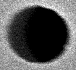
\includegraphics[scale=1.4]{Figures/original.png}};
  	\end{tikzpicture}
  }
\hfill
\subcaptionbox{Detektierte Umfangslinie (weiße Linie)\label{fig:kante}}
  [.3\linewidth]{
	\begin{tikzpicture}
        	\node (pixelsWithCircle) {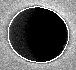
\includegraphics[scale=1.4]{Figures/originalMitKante.png}};
  	\end{tikzpicture}  
  }
\hfill
\subcaptionbox{Einzeichnung eines passenden Kreises mitsamt zugehörigem Radius\label{fig:eingezeichneterKreise}}
  [.3\linewidth]{
	\begin{tikzpicture}
        	\node[anchor=south west] (pixelsWithCircle) at (0,0) {
\includegraphics[scale=1.4]{Figures/edge.png}};
        	\begin{scope}[x={(pixelsWithCircle.south east)},y={(pixelsWithCircle.north west)}]
        	  \coordinate (R1) at (0.5,0.5);
        	  \coordinate (R2) at (0.85,0.5);
          \draw[green, ultra thick,->] (R1) -- (R2) node[midway,above]{$\SI{27}{px}$};
          \draw[green,ultra thick] (R1) ++(0:1.4cm) arc (0:360:1.4cm);
        \end{scope}
  	\end{tikzpicture}  
  }
	\caption{Von der Aufnahme zur Bestimmung der Umfangslinienlänge anhand der Kantenpixel}
\end{figure}

Mithilfe der Hough-Transformation kann die Position und der Radius eines in diese Kontur passenden Kreises bestimmt werden. Speziell für die Kontur in Abb. \ref{fig:kante} ergibt sich ein Kreis mit dem Radius $r_{\text{H,px}} = \SI{27}{px}$, welcher in Abb. \ref{fig:eingezeichneterKreise} als dicke Linie über der Kontur liegt.
Werden alle Konturenpixel zusammengezählt, ergibt sich eine Summe von $L_{\text{px}}= \SI{216}{px}$. Allerdings entspricht die Umfangslänge eines Kreises, der einen Radius von $\SI{27}{px}$ besitzt, lediglich der Länge $l_{\text{px}} = 2\pi\SI{27}{px} \approx \SI{167}{px}$, was einer relativen Abweichung von $\SI{27.1}{\percent}$ entspricht. Auch an dieser Stelle wird die Länge der Umfangslinie mithilfe der Kantenpixelzählung deutlich überschätzt.\\
Zusätzlich kann auch das Wissen um den Durchmesser der Löcher genutzt werden, um das Abschätzverfahren auf Tauglichkeit zu überprüfen. In Abschnitt \ref{sec:kalibrierungsfaktor} wurde der Begriff des Kalibrierungsfaktors eingeführt, mit dessen Hilfe die tatsächliche Länge in Mikrometern angegeben werden kann. Der in Abb. \ref{fig:ausschnitt} zu sehende Ausschnitt ist einer REM-Aufnahme entnommen, welche mit $25.000$-facher Vergrößerung eine Templatfolie zeigt. Diese Templatfolie ist mit Löchern perforiert, die einen normierten Durchmesser von $\SI{400}{\nm}$ besitzen. Aus diesen Informationen kann der zu erwartende Radius $r_{\text{H,px}}$ direkt mit $\SI{28.4}{px}$ angegeben werden\footnote{Der Maßstabsbalken im Bild ist auf $\SI{284}{px}$ pro $\SI{2}{\micro\metre}$ normiert. Erwarteter Radius der Löcher beträgt $\SI{0.2}{\micro\metre}$, was anhand des Maßstabes $\SI{28.4}{px}$ entspricht.}. Die daraus abgeleitete Umfangslänge liegt somit bei rund $\SI{178}{px}$, wodurch sich der relative Fehler der Abschätzung durch Pixelzählung auf $\SI{21}{\percent}$ verringert.

Im nächsten Abschnitt werden die Gründe für diesen Fehler und Möglichkeiten der Kompensation vorgestellt.\\

\subsection{Fehler durch Kreisrasterung}
Die Abweichung der Pixelzählung ist in der Diskretisierung des Kreisbogens begründet. Gerasterte horizontale oder vertikale Linien entsprechen in ihrer Abmessung exakt der zugrundeliegenden, geometrischen Form (Abb. \ref{fig:pixelHorizontal}). Kurvige und diagonal über das Gitter verlaufende Linien werden dagegen durch treppenartig angeordnete Pixel nur angenähert (Abb. \ref{fig:pixelDiagonal}) und benötigen deshalb insgesamt eine höhere Anzahl an Pixeln.\\

\def\pixelsHorizontal{
  {1,1,1,1,1,1,1,1,1,1,1},
  {1,1,1,1,1,1,1,1,1,1,1},
  {1,1,1,1,1,1,1,1,1,1,1},
  {1,0,0,0,0,0,0,0,0,0,1},
  {1,1,1,1,1,1,1,1,1,1,1},
  {1,1,1,1,1,1,1,1,1,1,1},
  {1,1,1,1,1,1,1,1,1,1,1}%
}

\def\pixelsDiagonal{
  {1,1,1,1,1,1,1,1,1},
  {1,1,1,1,1,1,1,0,0},
  {1,1,1,1,1,0,0,0,1},
  {1,1,1,1,0,0,1,1,1},
  {1,1,0,0,1,1,1,1,1},
  {1,0,0,1,1,1,1,1,1},
  {0,0,1,1,1,1,1,1,1}%
}

\begin{figure}[h!]
    \centering
    \begin{subfigure}[b]{0.475\textwidth}
        \centering
        \begin{tikzpicture}
	    \foreach \line [count=\y] in \pixelsHorizontal {
    			\foreach \pix [count=\x] in \line {
      			\draw[fill=pixel \pix] (\x/\scaleSmall,-\y/\scaleSmall) rectangle +(1/								\scaleSmall,1/\scaleSmall);
    			}
  		}
  		\draw[ultra thick,|<->|,red] (0.85,-1.4) -- (4.35,-1.4);
  		\draw (2.6,-.8) node[red,ultra thick,fill=white] {$l_{\text{px}}=\SI{9}{px}$};
  		\draw (2.6,-2) node[black,ultra thick,fill=white] {$L_{\text{px}}=\SI{9}{px}$};
        \end{tikzpicture}
        \caption{Hier entspricht die Länge der Pixel genau der zugrundeliegenden Linie ($\SI{1}{Pixel} \equiv \SI{1}{px}$)}
        \label{fig:pixelHorizontal}
    \end{subfigure}
    \hfill
    \begin{subfigure}[b]{0.475\textwidth}
        \centering
        \begin{tikzpicture}[label distance=10mm]
        \foreach \line [count=\y] in \pixelsDiagonal {
    			\foreach \pix [count=\x] in \line {
      			\draw[fill=pixel \pix] (\x/\scaleSmall,-\y/\scaleSmall) rectangle +(1/								\scaleSmall,1/\scaleSmall);
    			}
  		}
  		\coordinate (A) at (0.6,-2.65);
  		\coordinate (B) at (3.85,-.6);
  		\draw [red,ultra thick,|<->|]   (A) to[out=45,in=200] (B);
  		\draw (1.37,-.8) node[red,ultra thick,fill=white] {$l_{\text{px}}=\SI{9}{px}$};
  		\draw (2.9,-2.0) node[black,ultra thick,fill=white] {$L_{\text{px}}=\SI{12}{px}$};
        \end{tikzpicture}
        \caption{Dieses kurvige Bogenstück ist ein Ausschnitt der Kontur aus Abb. \ref{fig:kante} ($\SI{1}{Pixel} \equiv \SI{0.7}{px}$) }
        \label{fig:pixelDiagonal}
    \end{subfigure}
    \caption{Vergleich zwischen Rasterungen einer horizontalen Linie und einer diagonal verlaufenden Linie. Die Rasterung in (b) benötigt signifikant mehr Pixel.}
\end{figure}

Finden sich in dem zu analysierenden Bild eine hohe Anzahl an kurvigen Formen, so kann ohne Berücksichtigung des Diskretisierungsfehlers nicht ohne Weiteres die Kantenpixelanzahl als tatsächliche Länge aller Kurvenstücke bestimmt werden. 
Um die Auswirkung des Diskretisierungsfehlers abschätzen und kompensieren zu können, wird in Tabelle \ref{tab:kantenlängenEinzelnerLöcher} eine Vielzahl von unterschiedlichen Kreisen der gleichen Aufnahme (Abb. \ref{fig:appendix1}) auf Anzahl der Kantenpixel und den durch die Abschätzung verursachten Fehler untersucht.\\
Beachte: Die einzelnen Löcher werden in den Tabellen \ref{tab:kantenlängenEinzelnerLöcher}, \ref{tab:kantenlängenEinzelnerLöcher2} und \ref{tab:einzelneLöcher3} über den Identifier "<Abbildungsnummer>.<Lochnummer>" referenziert. Die Abbildungen sind dem Anhang beigefügt.

Die beiden Fehler-Größen $f_{\text{H}}$ und $f_{\text{D}}$ bilden den prozentualen Fehler der Schätzmethode bezüglich der geometrischen Umfangslinienlängen $l_{\text{H,px}}$ und $l_{\text{D,px}}$, welche einerseits über die Hough-Transformation und andererseits über die Angaben zum Lochdurchmesser aus dem Datenblatt bestimmt werden.

\begin{align}
f_H = \frac{L_{\text{px}}-l_{\text{H,px}}}{l_{\text{H,px}}}\SI{100}{\percent} && f_D = \frac{L_{\text{px}}-l_{\text{D,px}}}{l_{\text{D,px}}}\SI{100}{\percent}
\end{align}

\begin{table}[h!]
	\caption{Ergebnisse der Untersuchung einzelner Löcher aus Abb. \ref{fig:appendix1} auf Kantenpixelanzahl und daraus resultierende  Abschätzungsfehler in Bezug auf den ermittelten Radius $r_{\text{H,px}}$ als auch auf den im Vorfeld bekannten Radius $r_{\text{D,px}} = \SI{28.4}{px}$. Ermittelt wird $r_{\text{H,px}}$ mithilfe der Hough Transformation. Entsprechend ist $f_{\text{H}}$ der prozentuale Fehler in Bezug auf $r_{\text{H,px}}$ und $f_{\text{D}}$ der prozentuale Fehler in Bezug auf $r_{\text{D,px}}$. Weiter bezeichnet $\overline{x}$ den Mittelwert, $s_x$ die emp. Standardabweichung und $v_s$ den emp. Variationskoeffizienten der Messreihe. Letztere sollen die Beurteilung hinsichtlich eines systematischen Fehlers vereinfachen.}
	\centering
	\begin{tabular}{cccS[table-format=3.1]S[table-format=3.1]}
		\toprule
							&						&\multicolumn{2}{c}{\textbf{Hough-T.}}\\
		\cmidrule(rr){3-4}
		\textbf{Loch}		&\textbf{$L_{\text{px}}$}	&$r_{\text{H,px}}$		&$f_H$ 	&$\textbf{$f_D$}$\\
		\midrule
			B1.1				&202						&30					&7.2						&13.2\\
			B1.2				&209						&27					&23.2  					&17.1\\
			B1.3				&198						&26					&21.2					&11.0\\
			B1.4				&211						&30					&11.9					&18.2\\
			B1.5				&206						&27					&21.4  					&15.4\\
			B1.6				&184						&25					&17.1					&3.1\\
			B1.7				&204						&26					&24.9					&14.3\\
			B1.8				&209						&30					&10.9					&17.1\\
		\midrule
			$\overline{x}$	&203						&27.6				&17.2					&13.7\\
			$s_x$			&8,7						&2,1					&6.5						&4.9\\
			$v_s$			&						&					&37.8					&35.7\\
		\bottomrule
	\end{tabular}
	\label{tab:kantenlängenEinzelnerLöcher}
\end{table}

Weichen die Ergebnisse dieser Methode systematisch ab, können diese mithilfe eines Anpassungsfaktors effektiv kompensiert werden und zu einem befriedigenden Ergebnis führen. Die Frage, ob ein systematischer Fehler vorliegt, kann mithilfe der empirischen Standardabweichung $s_x$ und dem Varianzkoeffizienten $v_s$ (Definition \ref{eq:varkof}) als Streuungsmaß beantwortet werden. 

\begin{equation}
v_s = \frac{s_x}{\overline{x}}
\label{eq:varkof}
\end{equation}

Systematische Abweichungen erzeugen eine Verschiebung nach einer Seite, also eine Tendenz stets zu hohen oder zu niedrigen Messwerten [Quellenverweis zu betreffendem Wiki-Artikel]. In Tabellen \ref{tab:kantenlängenEinzelnerLöcher}, \ref{tab:kantenlängenEinzelnerLöcher2} und \ref{tab:einzelneLöcher3} wird aus den Fehlern direkt ersichtlich, dass hier eine eben solche einseitige Tendenz zu hohen Abweichungen vorliegt. Um allerdings den Begriff einer systematischen Abweichung enger zu fassen, wird die innere Genauigkeit dieser Abweichung mithilfe des Varianzkoeffizienten $v_s$ näher untersucht. Nach [Quellenverweis auf die englische Wiki-Seite zu Varianzkoeffizient] gelten Verteilungen als gering gestreut, wenn deren Varianzkoeffizient unter \SI{100}{\percent} liegt und als hoch gestreut, wenn diese einen Varianzkoeffizienten von über \SI{100}{\percent} aufweisen.\\
Im Rahmen dieser Untersuchung wird willkührlich festgelegt, dass eine systematische Abweichung genau dann vorliegt, wenn der Varianzkoeffizient der Messreihe bei unter \SI{100}{\percent} liegt, also eine hohe innere Genauigkeit aufweist. Dies ist in den Untersuchungen für die Aufnahmen \ref{fig:appendix2} und \ref{fig:appendix3} der Fall, so dass davon ausgegangen werden kann, dass hier eine systematische Abweichung vorliegt. Weiter lässt sich aus den Ergebnissen schlussfolgern, dass sich die Tendenz zur systematischen Abweichung bei Aufnahmen von Löchern aus großen Rastergittern entwickelt.

\paragraph{Unterschiedliche Kreisdurchmesser}
Um festzustellen, ob es einen Zusammenhang zwischen Rastergitter-Größe, resultierenden Fehlern und deren Streuung gibt, werden zusätzlich Löcher aus Aufnahmen unterschiedlicher Zoom-Stufen untersucht (siehe Abb. \ref{fig:appendix1} und Abb. \ref{fig:appendix3}). Die hieraus entstandenen Ergebnisse in Tabellen \ref{tab:kantenlängenEinzelnerLöcher2} und \ref{tab:einzelneLöcher3} sollen Aufschluss darüber geben, ob Abschätzungsfehler durch die Wahl des Zoomlevels beeinflussbar sind.\\

\begin{table}[h!]
	\parbox{.45\linewidth}{
	\centering
	\caption{Untersuchsreihe zu Löchern im kleinen Maßstab in Bezug auf Abb. \ref{fig:appendix2}. Der bekannte Lochradius beträgt hier $r_{\text{D,px}} = \SI{16.8}{\pixel}$.}
	\begin{tabular}{cccS[table-format=3.1]S[table-format=3.1]}
		\toprule
							&						&\multicolumn{2}{c}{\textbf{Hough-T.}}\\
		\cmidrule(rr){3-4}
		\textbf{Loch}		&\textbf{$L_{\text{px}}$}	&$r_{\text{H,px}}$		&$f_H$ 	&$\textbf{$f_D$}$\\
		\midrule
			B2.1				&120						&18					&6.1					  	&13.7\\
			B2.2				&115						&14					&30.7  					&8.9\\
			B2.3				&114						&18					&0.8						&8.0\\
			B2.4				&104						&17					&-2.6					&-1.5\\
			B2.5				&104						&12					&37.9  					&-1.5\\
			B2.6				&119						&19					&-0.3					&12.7\\
			B2.7				&103						&13					&26.1					&-2.4\\
			B2.8				&119						&14					&35.3					&12.7\\
		\midrule
			$\overline{x}$	&112						&15,6				&16,7					&6.3\\
			$s_x$			&7,4						&2,7					&17.4					&7.0\\
			$v_s$			&						&					&103.7					&110.6\\
		\bottomrule
	\end{tabular}
	\label{tab:kantenlängenEinzelnerLöcher2}
	}
	\hfill
	\parbox{.45\linewidth}{
	\centering
	\caption{Untersuchsreihe zu Löchern im großen Maßstab in Bezug auf Abb. \ref{fig:appendix3}. Der bekannte Lochradius beträgt hier $r_{\text{D,px}} = \SI{74.4}{\pixel}$.} 
	\begin{tabular}{cccS[table-format=3.1]S[table-format=3.1]}
		\toprule
							&						&\multicolumn{2}{c}{\textbf{Hough-T.}}\\
		\cmidrule(rr){3-4}
		\textbf{Loch}		&\textbf{$L_{\text{px}}$}	&$r_{\text{H,px}}$		&$f_H$ 	&$\textbf{$f_D$}$\\
		\midrule
			B3.1				&561						&77					&16.0					&20.0\\
			B3.2				&553						&77					&14.3  					&18.3\\
			B3.3				&597						&79					&20.3					&27.7\\
			B3.4				&547						&78					&11.6					&17.0\\
			B3.5 			&565						&77					&16.8  					&20.9\\
			B3.6				&577						&78					&17.7					&23.4\\
			B3.7				&554						&76					&16.0					&18.5\\
			B3.8				&575						&78					&7.3						&23.0\\
		\midrule
			$\overline{x}$	&566						&77,5				&15.0					&21,1\\
			$s_x$			&16,3					&0,9					&4.0						&3,5\\
			$v_s$			&						&					&26.7					&16.6\\
		\bottomrule
	\end{tabular}
	\label{tab:einzelneLöcher3}
	}
\end{table}

Es kann festgestellt weren, dass die prozentualen Messabweichungen $f_H$ und $f_D$ systematisch größer werden, je größer die zu untersuchenden Löcher auf der Aufnahme abgebildet sind. Gleichzeitig stabilisieren sich sowohl Streuung als auch der Varianzkoeffizient mit steigendem Abbildungsmaßstab. Umgekehrt wird der Varianzkoeffizient für Aufnahmen kleinen Maßstabs beliebig groß. Er liegt in diesem Fall bei über \SI{100}{\percent} und macht damit eine sinnvolle Fehlerkompensation nahezu unmöglich.\\

\subsection{Fehlerkompensation}
Im vorherigen Abschnitt wurde gezeigt, dass die systematische Abweichung mit der Abbildungsmaßstab der Aufnahme der korreliert. Um diese Abweichung kompensieren zu können, wird ein Korrekturfaktor $k_D$ eingeführt, der direkt über den Mittelwert des Fehlers $f_{\text{D}}$ bestimmt wird.

\begin{equation}
k_D := \frac{1}{1+\frac{\overline{f_D}}{\SI{100}{\percent}}}
\label{def:kompensation}
\end{equation}

Auf diese Weise kann die Summe der gezählten Kantenpixel $L_{\text{px}}$ direkt mit dem Korrekturfaktor $k_D$ nach unten korrigiert werden, um den neuen Schätzwert $\hat{L}_{\text{px}}$ für die Umfangslinienlänge $l_{\text{px}}$ zu erhalten.

\begin{equation}
\hat{L}_{\text{px}} = k_DL_{\text{px}}
\end{equation}

\subsection{Vor- und Nachteile}
Ein wesentlicher Vorteil der Methode der Kantenpixelzählung ist die Ausführungsgeschwindigkeit. Zeitmessungen hierzu folgen in Tabellen \ref{tab:ergebnisseHelligkeit}, \ref{tab:ergebnisseKontrast} und \ref{tab:ergebnisseAuflösung} in Kapitel \ref{ch:vergleichDerErgebnisse}.\\
Ein weiterer Vorteil dieses Verfahrens ist die Berücksichtigung von Objekten am Rande eines Bildes. Bei der Hough-Transformation dagegen werden Löcher, deren Mittelpunkt nicht mehr im Bildbereich detektierbar sind, vernachlässigt, wodurch ein nicht vernachlässigbarer Fehler entsteht.

Nachteilig wirkt sich der (systematische) Schätzfehler durch Verwendung einer zum Messergebnis führenden Beziehung zwischen Größen, die der tatsächlichen Verknüpfung nicht entspricht. Explizit geht es dabei um die Verknüpfung $L_{\text{px}} \equiv l_{\text{px}}$, die in Wirklichkeit nicht gegeben ist. Da bei ausreichend großen Strukturen in der Aufnahme eine systematische Abweichung dieser Verknüpfung angenommen werden kann, wurde in Gleichung \ref{def:kompensation} der Korrekturfaktor $k_D$ definiert, um über eine neue Verknüpfung $k_DL_{\text{px}} \equiv l_{\text{px}}$ den Schätzfehler der Umfangslinienlänge zu kompensieren.\\
Ein weiterer Nachteil der Kantendetektion ist die Empfindlichkeit gegenüber Rauschen des Bildsensors und physischen Artefakten auf der zu untersuchenden Oberfläche. Unebenmäßigkeiten auf der Substratgrundfläche werden ebenfalls als Kantenpixel extrahiert und fälschlicherweise zur Umfangslinienlänge hinzugenommen.

\chapter{Ergebnisse und Vergleich}
\label{ch:vergleichDerErgebnisse}
Im Verlauf dieser Arbeit wurden zwei Möglichkeiten der Oberflächenerfassung vorgestellt. Welche für den vorliegenden Anwendungsfall die geeignetere ist, wird in diesem Kapitel untersucht.
\section{Festlegung der Bewertungskriterien}
Folgende Punkte sollen als  Vergleichskriterien dienen:
\begin{itemize}
\item \textbf{Robustheit}\\ 
Das Verfahren ist robust gegenüber verschiedenen Bildaufnahmeeinstellungen, Auflösung und Größe der zu detektierenden Kreise. Zusätzlich werden diese Kriterien nicht nur unter einer einzigen Bildaufnahme verglichen, sondern auch mit unterschiedlichen Aufnahmeparametern gegenübergestellt.\\
Mithilfe der Einstellungen, welche direkt bei der Aufnahme am REM ausgewählt werden können, wurden für die Gegenüberstellung folgende Werte in drei äquidistanten Stufen für den Vergleich herangezogen:
\begin{itemize}
\item \textbf{Helligkeit}\\ 
\item \textbf{Kontrast}\\
\item \textbf{Auflösung} \\
\end{itemize}
\item \textbf{Korrekte Anzahl detektierter Kreise}\\
Das Maß an korrekt detektierten Kreisen gegenüber der tatsächlich vorliegenden Menge. Hierbei wird die Anzahl ausgelassener Kreise (unter der Spalte "M" in den folgenden Vergleichstabellen) und die Anzahl von falsch positiven Detektionen (Spalte "FP") gegenübergestellt. 
\item \textbf{Zeitperformance} \\
Die benötigte Zeit zur Berechnung der Mantelfläche $F$ in Sekunden.
\end{itemize}

Als Referenzwert für die Gegenüberstellung wird aufgrund der sehr präzisen Ergebnisse in den Versuchsreihen das Verfahren der Hough-Transformation mit der gekoppelten geometrischen Umfangslinienberechnung gewählt. Damit soll vor allem überprüft werden, ob das Maß an Zeiteinsparung die ungenauere Oberflächenberechnung durch den pixelbasierten Ansatz kompensiert werden kann\footnote{Allerdings spielt im Rahmen der Aufgabenstellung dieser Arbeit der Zeitkostenpunkt eine untergeordnete Rolle, da nur eine relativ begrenzte Anzahl an Bildern zur Verfügung steht.}.

\section{Ergebnisse}
Nachfolgend werden sämtliche Messergebnisse hinsichtlich berechneter Mantelfläche $F$ beider in Kapitel \ref{ch:umfangsberechnung} vorgestellten Schätzmethoden aufgeführt. Alle Durchläufe wurden dabei im \textit{single-thread}-Modus direkt in Matlab ausgeführt. Die Zeitperformance kann sich von Rechnerarchitektur zu Rechnerarchitektur unterscheiden und soll lediglich einen groben Anhaltspunkt für die benötigte Zeit geben.

\subsection{Variation der Helligkeit}
Für die folgende Gegenüberstellung werden die Verfahren auf Robustheit im Bezug auf Helligkeitsveränderungen untersucht. Als Grundlage dienen die Aufnahmen in Abb. \ref{fig:helligkeitsreihe}.\\

\begin{figure}[H]
\centering
\subcaptionbox{Niedrige Helligkeit (B35.2)\label{fig:helligkeitNiedrig}}%
  [.3\linewidth]{
  	\begin{tikzpicture}
        	\node (pixelsWithCircle) {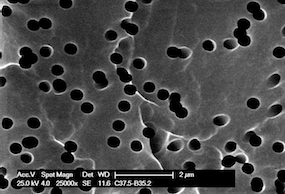
\includegraphics[scale=0.9]{Figures/111.png}};
  	\end{tikzpicture}
  }
\hfill
\subcaptionbox{Mittlere Helligkeit (B38.2)\label{fig:helligkeitMittel}}%
  [.3\linewidth]{
	\begin{tikzpicture}
        	\node (pixelsWithCircle) {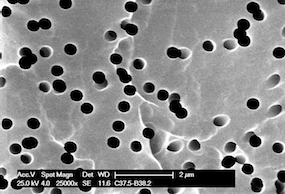
\includegraphics[scale=0.9]{Figures/110.png}};
  	\end{tikzpicture}  
  }
\hfill
\subcaptionbox{Hohe Helligkeit (B41.2)\label{fig:helligkeitHoch}}%
  [.3\linewidth]{
	 \begin{tikzpicture}
        	\node (pixelsWithCircle) {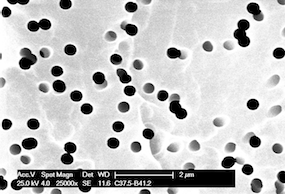
\includegraphics[scale=0.9]{Figures/109.png}};
  	\end{tikzpicture} 
  }
\caption{Von der Aufnahme zur Bestimmung der Umfangslinienlänge anhand der Kantenpixel}
\label{fig:helligkeitsreihe}
\end{figure}

\begin{table}[H]
	\caption{Ergebnisse hinsichtlich verschiedener Helligkeitseinstellungen. Hierbei bezeichnet $G_A$ den generisch bestimmten Sensitivitätswert (s. Abschnitt \ref{ssec:sensitivitätsberechnung})  und $G_H$ denjenigen, der manuell durch Ausprobieren gewählt wurde. Weiter bezeichnet $F$ die berechnete Mantelfläche, welche der Innenseite der Poren der Template entsprechen. M (missed) steht für die Anzahl nicht detektierter Löcher und FP (false positive) für die Anzahl von Falschdetektionen. Als $f_{\text{geo}}$ wird der prozentuale Fehler der berechneten Mantelfläche $F_{\text{px}}$ der pixelbasierten Methode im Bezug zur berechneten Fläche $F$ der geometrischen Methode bezeichnet.}
	\centering
	\begin{tabular}{ccccccccS[table-format=2.1]}
		\toprule	
							&\multicolumn{5}{c}{\textbf{Geom. Ansatz}}	&\multicolumn{3}{c}{\textbf{Pixelbasiert}}\\
		\cmidrule(rr){2-6} \cmidrule(rr){7-9}
			\textbf{Helligkeit} &	Sensitivität	&\text{$F$ ($\SI{}{\micro\metre}^2$)} &M &FP 	&Zeit (s)	&\text{$F_{\text{px}}$ ($\SI{}{\micro\metre}^2$)}	&Zeit (s)	&$\text{$f_{\text{geo}}$}$ \\
		\midrule
			B35.2	&$G_A = 0.940$		&995		&6	&7	&3,01			&				&			&\\
					&$G_H = 0.940$		&995		&6	&7	&3,01			&1033			&$\ll1$			&3.8\\
			B38.2	&$G_A = 0.915$		&788		&8	&0	&3,06			&				&			&\\
					&$G_H = 0.930$		&882		&1	&0	&3,22			&1228			&$\ll1$				&39.2\\
			B41.2	&$G_A = 0.880$		&624		&19	&0	&2,42			&				&			&\\
					&$G_H = 0.925$		&880		&2	&0	&2,90			&1422			&$\ll1$			&61.6\\
		\bottomrule
	\end{tabular}
	\label{tab:ergebnisseHelligkeit}
\end{table}

\subsection{Variation des Kontrasts}

\begin{figure}[H]
\centering
\subcaptionbox{Niedriger Kontrast (C32.5)\label{fig:kontrastNiedrig}}%
  [.3\linewidth]{
  	\begin{tikzpicture}
        	\node (pixelsWithCircle) {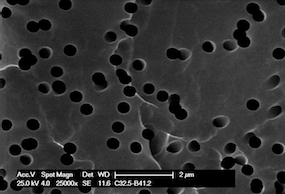
\includegraphics[scale=0.9]{Figures/108.png}};
  	\end{tikzpicture}
  }
\hfill
\subcaptionbox{Mittlerer Kontrast (C35.5)\label{fig:kontrastMittel}}%
  [.3\linewidth]{
	\begin{tikzpicture}
        	\node (pixelsWithCircle) {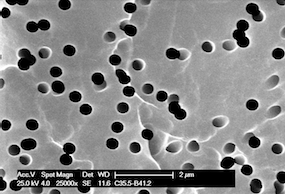
\includegraphics[scale=0.9]{Figures/107.png}};
  	\end{tikzpicture}  
  }
\hfill
\subcaptionbox{Hoher Kontrast (C37.5)\label{fig:kontrastHoch}}%
  [.3\linewidth]{
	 \begin{tikzpicture}
        	\node (pixelsWithCircle) {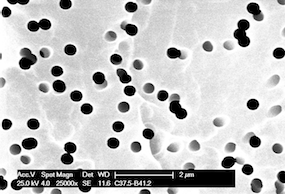
\includegraphics[scale=0.9]{Figures/109.png}};
  	\end{tikzpicture} 
  }
\caption{Von der Aufnahme zur Bestimmung der Umfangslinienlänge anhand der Kantenpixel}
\label{fig:kontrastreihe}
\end{figure}

\begin{table}
	\caption{Ergebnisse hinsichtlich verschiedener Kontrasteinstellungen}
	\centering
	\begin{tabular}{ccccccccS[table-format=2.1]}
		\toprule	
							&\multicolumn{5}{c}{\textbf{Geom. Ansatz}}	&\multicolumn{3}{c}{\textbf{Pixelbasiert}}\\
		\cmidrule(rr){2-6} \cmidrule(rr){7-9}
			\textbf{Kontrast} &	Sensitivität	&\text{$F$ ($\SI{}{\micro\metre}^2$)} &M &FP 	&Zeit (s)	&\text{$F_{\text{px}}$ ($\SI{}{\micro\metre}^2$)}	&Zeit (s)	&$\text{$f_{\text{geo}}$}$ \\
		\midrule
			C32.5	&$G_A = 0.925$		&859		&6	&1	&3,12			&				&			&\\
					&$G_H = 0.925$		&859		&6	&1	&3,12			&1465			&$\ll1$		&70.5\\
			C35.5	&$G_A = 0.935$		&925		&0	&0	&3,06			&				&			&\\
					&$G_H = 0.935$		&925		&0	&0	&3,42			&1366			&$\ll1$			&46.1\\
			C37.5	&$G_A = 0.880$		&624		&19	&0	&2,42			&				&			&\\
					&$G_H = 0.925$		&880		&2	&0	&2,90			&1422			&$\ll1$			&61.6\\
		\bottomrule
	\end{tabular}
	\label{tab:ergebnisseKontrast}
\end{table}

\subsection{Auflösung}

\begin{table}[h!]
	\caption{Ergebnisse hinsichtlich verschiedener Auflösungen der Aufnahme in Abb. \ref{fig:kontrastMittel}}
	\centering
	\begin{tabular}{ccccccccS[table-format=2.1]}
		\toprule	
							&\multicolumn{5}{c}{\textbf{Geom. Ansatz}}	&\multicolumn{3}{c}{\textbf{Pixelbasiert}}\\
		\cmidrule(rr){2-6} \cmidrule(rr){7-9}
			\textbf{Auflösung} &	Sensitivität	&\text{$F$ ($\SI{}{\micro\metre}^2$)} &M &FP 	&Zeit (s)	&\text{$F_{\text{px}}$ ($\SI{}{\micro\metre}^2$)}	&Zeit (s)	&$\text{$f_{\text{geo}}$}$ \\
		\midrule
			C35.5$(.5\times)$	&$G_A = 0.940$		&888		&2	&0	&0,67			&				&			&\\
						&$G_H = 0.940$			&888		&2	&0	&0,67			&1025			&$\ll1$				&15.4\\
			C35.5$(1\times)$	&$G_A = 0.935$		&925		&0	&0	&3,06			&				&			&\\
					&$G_H = 0.935$		&925		&0	&0	&3,42			&1366			&$\ll1$			&46.1\\
			C35.5$(2\times)$	&--			&--		&--	&--	&--				&				&			&\\
						&$G_H = 0.945$			&894		&1	&0	&21,25			&1241			&$\ll1$				&38.8\\
		\bottomrule
	\end{tabular}
	\label{tab:ergebnisseAuflösung}
\end{table}

\section{Fazit}
Wie erwartet hat im besonderen Maße die geometrische Methode die besten Ergebnisse hinsichtlich einer genauen Flächenberechnung gezeigt. Die pixelbasierte Methode konnte bestenfalls bei guten Helligkeits- und Kontrastwerten mit einem kleinen Fehler eine gute Näherung geben. In allen anderen Fällen ist die Abweichung durch bloße Kantenlängenzählung mit durchgeführter Kompensation zu hoch, um praktischen Einsatz finden zu können. Die Zeiteinsparung ist bei den auftretenden kurzen Durchlaufzeiten gegenüber dem geometrischen Pendant vernachlässigbar.\\

Wünschenswert war die Übereinstimmung der Sensitivitätswerte $G_A$ und $G_H$, da dies mit einer erfolgreichen, vollautomatischen Parameterberechnung gleichzusetzen ist. $G_H$ kann damit auch stets als Referenzwert für den generisch ermittelten Arbeitspunkt $G_A$ angesehen werden.\\
In dieser Hinsicht war die Qualität des generischen Ansatzes für eine Vielzahl von Bildern sehr zufriedenstellend. Eine relativ starke Abweichung trat nur bei sehr hellen Bildern auf (siehe Abb. \ref{fig:helligkeitHoch} und Abb. \ref{fig:kontrastHoch} sowie Tabelle \ref{tab:ergebnisseHelligkeit}, letzter Eintrag).

Das Bild mit den günstigsten Aufnahmeparametern war jenes aus Abbildung \ref{fig:kontrastMittel}. Bei dieser Aufnahme wurden sowohl alle sichtbaren Kreise als auch keine falsch positiven Ergebnisse detektiert. Zusammenfassend kann die Aussage getroffen werden, dass Aufnahmen für eine möglichst genaue Flächenberechnung eine mittlere Helligkeit und einen mittleren Kontrast aufweisen sollen.

Auffällig in diesen Messreihen war die starke Korrelation zwischen Bildauflösung und Ausführungszeit. Eine einzelne Kreisdetektion bei doppelter Auflösung hat die Ausführungszeit um den Faktor 7 erhöht. Aus diesem Grund war eine Zeitmessung mit generisch bestimmtem Sensitivitätswert $G_A$ zeitlich nicht möglich, da der Zeitaufwand der Iterationen über den Arbeitsbereich die in der Praxis verfügbare Zeit deutlich überstieg. 
Auch hier ist eine mittlere Auflösung von etwa $1000\times2000$ vorzuziehen. Auflösungen unter diesem Ankerpunkt erzeugen eine größere Abweichung als Auflösungen darüber. Folglich ist eine niedrige Auflösung stets zu vermeiden.

Insgesamt kann die Arbeit mit dem Urteil geschlossen werden, dass eine hinreichend genaue geometrische Oberflächenbestimmung von REM-Aufnahmen mit dem Ansatz der Hough-Transformation und der trigonometrischen Berechnung aller Umfangslinien durchführbar ist.

\chapter{Weiterführende Arbeit}
\section{Allgemeine Hough-Transformation}
Eine weitere Möglichkeit zur Lösung des Detektionsproblems über den geometrischen Ansatz ist der Einsatz der generalisierten Hough-Transformation [13]. Hier würde sich beispielsweise die Parametrisierung einer halben Ellipse anbieten, da sich innerhalb der Versuchsreihen immer wieder gezeigt hatte, dass durch eine Kantenextraktion viele halbe Ellipsen hervortreten. Diese entstanden meist durch seitliche Ionenbeschüsse, so dass bei der Aufnahme einseitige Verschmierungen durch unzureichenden Kontrast zwischen Lochinnenseite und Lochumriss entstanden. In einem mehrstufigen Prozess könnte man auf diese Weise die Genauigkeit der detektierten Lochpositionen unter einem kleineren Schwellenwert realisieren.

\section{Hinzunahme weiterer quantifizierbarer Größen}
Eine Verbesserung des Kreisdetektions-Algorithmus kann durch Hinzunahme weiterer, extrahierbarer Informationen noch verbessert werden. Beispielsweise kann der Ausgabeparameter \lstinline|metric| der Funktion \lstinline|imfindcircles| angeführt werden. Dieser sortiert die gefundenen Kreise in einer absteigenden Reihenfolge anhand ihrer Kantenstärke. Aus diesen Größen kann der Zusammenhang zu nicht orthogonal geschossenen Löchern hergestellt werden. Löcher, die durch einen seitlichen Einschuss entstehen, erscheinen beim Detektionsvorgang als unfertige Bogensegmente und landen damit im \lstinline|metric|-Array sehr weit unten. Das ist deshalb wichtig, weil ein nicht orthogonal erzeugtes Loch einen verzogenen Umriss aus Perspektive des Mikroskopobjektivs besitzt und das damit sowohl die geometrische als auch die pixelbasierte Umfangs- und Oberflächenberechnung erschwert.

\section{Parallelisierung des Algorithmus}
Die vorliegende Implementierung der Arbeitspunktsuche ist so geschrieben, dass jede Iteration entlang des Sensitivitätsbereich von einem einzigen Prozess (Thread) berechnet wird. Da die Kreisdetektion für unterschiedliche Sensitivitätswerte jedoch vollkommen unabhängig voneinander ablaufen, können theoretisch beliebig viele Einzeliterationen in unterschiedlichen Prozessen abgearbeitet und damit insgesamt deutlich beschleunigt werden.

\section{Machine Learning}
Das Fachgebiet des Maschinellen Lernens bietet die Möglichkeit bereits detektierte Strukturen auf ihre korrekte Erkennung zu überprüfen. Dazu könnten mithilfe eines Trainingssets, welches unterschiedliche Ausschnitte von Löchern einer Templatfolie beinhaltet, ein Klassifizierungsmodell erstellt werden. Dieses ist dann in der Lage eine Wahrscheinlichkeit anzugeben, ob die untersuchte Struktur einem Kreis entspricht. 
Diese Vorgehensweise setzt jedoch die bereits detektierten Kreise voraus und ist nicht in der Lage von sich aus die Positionen der Kreise zu erfassen. Dementsprechend hat die Klassifizierung einer eher unterstützende Aufgabe bei der Verifizierung der Ergebnisse.
Nachteile treten in Form von hoher Sensibilität für Variationen in Lichtverhältnissen, Rotation und Skalierung des Kreises auf. Deshalb müssen die Bedingungen unter denen die Bilder aufgenommen werden, sehr präzise kontrolliert werden.

\chapter{Literaturverzeichnis}

{[1]} \textsc{Hough, P. V. C}. \textit{Method and means for recognizing complex patterns}. US Patent, 1962.\\

{[2]} \textsc{Canny, J. F}. \textit{A computational approach to edge detection}. S. 679-698, 1986.\\

{[3]} \textsc{Burger, W., Burge, M. J}. \textit{Digitale Bildverarbeitung}. Springer-Verlag Berlin, 2006\\

{[4]} \textsc{Atherton, T. J., Kerbyson, D. J}. \textit{Image and Vision Computing}. Volume 17, Number 11, 1999.\\

{[5]} \textsc{Brunelli, R.}. \textit{Template Matching Techniques in Computer Vision: Theory and Practise}. Wiley, 2009.\\

{[6]} \textsc{Speiser, B.}. \textit{Cyclische Voltammetrie}. 1981.\\

{[7]} \textsc{Bradski, G., Kaehler, A.}. \textit{Learning OpenCV Computer Vision with the OpenCV Library}. O'Reilly, 2008.\\

{[8]} \textsc{Mathworks.com}. \textit{Image Processing Toolbox}. MATLAB and Simulink [Internet], verfügbar auf: https://de.mathworks.com/products/image.html.\\

{[9]} \textsc{Mathworks.com}. \textit{Detect and Measure Circular Objects in an Image}. MATLAB and Simulink [Internet], 2013, verfügbar auf: http://www.mathworks.com/help/images/examples/detect-and-measure-circular-objects-in-an-image.html.\\

{[10]} \textsc{Marr, D.}. \textit{Vision}. Freeman, 1982.\\

{[11]} \textsc{Baumann, R}. \textit{Geometrie: Winkelfunktionen, Trigonometrie}. S.76-77, Mentor, 1999.\\

{[12]} \textsc{Bresenham, J. E}. \textit{A Linear Algorithm for Incremental Digital Display of Circular Arcs}. S.100-106, 1977.\\

{[13]} \textsc{Ballard, D. H., Brown, C. M}. \textit{Computer Vision}. Prentice-Hall, 1982.\\
	
%************* Verzeichnisse ************
\clearpage
%****************************************


	%****************************************
%Anhang
%****************************************	
\appendix
\addcontentsline{toc}{chapter}{Anhang}
\chapter{Code}
\section{calculateSurfaceByDIP.m}
\begin{lstlisting}[language=MATLAB, caption=Verfeinerung der lokalen Minima, label=lst:calculateSurfaceByDIP]
function [surface,sensitivity] = calculateSurfaceByDIP(varargin)
%CALCULATESURFACEBYDIP Calculate surface of cylindric objects
%   SURFACE = CALCULATESURFACEBYDIP(IMAGE) calculates the surface of cylindric
%   objects in the input image IMAGE. IMAGE can be a grayscale, RGB or
%   binary image. SURFACE is calculated by the position of found circles,
%   the default cylinder height of 24 micrometers and the default scale
%   factor of 1/142 micrometers per pixel.
%
%   [SURFACE, SENSITIVITY] = CALCULATESURFACEBYDIP(IMAGE) returns the
%   determined SENSITIVITY used for locating circle positions. Can be
%   useful for calibration of a series of images of the same record
%   parameters.
%
%   SURFACE = CALCULATESURFACEBYDIP(...,PARAM1,VAL1,PARAM2,VAL2,...)
%   calculates surface using name-value pairs to control aspects of the
%   Circular Hough Transform, scaling and visualization. Parameter names
%   can be abbreviated.
%
%   Parameters include:
%
%   'ObjectPolarity' - Specifies the polarity of the circular object with
%                      respect to the background. Available options are:
%
%                      'bright' : The object is brighter than the background.
%                      'dark'   : The object is darker than the background. (Default)
%
%   'Method' - Specifies the technique used for computing the operation
%              point. Available options are:
%
%              'BinarySearch'  : Binary search to find the operation range.
%                                (Default)
%              'QuickEstimate' : Very quick method to find a mediocre
%                                operation range
%
%   'Sensitivity ' - Specifies the sensitivity factor in the range [0 1]
%                    for finding circles. A high sensitivity value leads
%                    to detecting more circles, including weak or
%                    partially obscured ones, at the risk of a higher
%                    false detection rate. Default value: Computed by the
%                    method which is specified by the 'Method' param.
%
%   'ScaleFactor' - Specifies how many pixels are needed to match one
%                   micrometer.
%                   Some values for specific zoom levels:
%                    8000x : 0.0219/1.4
%                   15000x : 0.012/1.4
%                   20000x : 0.0088/1.4
%                   25000x : 0.0071/1.4 (default)
%                   65000x : 0.0027/1.4
%                       yx : 175.2/y/1.4
%
%   'Height' - HEIGHT overrides the default HEIGHT of the cylinders.
%              Unit: micrometer.
%
%   'Visualization' - Specifies the visualization of found circles and arcs
%                     in the original image.
%
%                     'on' : Activate visualization
%                     'off' : Deactivate visualization (default)
%
%   Notes
%   -----
%   1.  Binary images (must be logical matrix) undergo additional pre-processing
%       to improve the accuracy of the result. RGB images are converted to
%       grayscale using RGB2GRAY before they are processed.
%   2.  Accuracy is limited for very small radius values, e.g. Rmin <= 5.
%   3.  The sensitivity estimation step for QuickSearch method is typically
%       faster than that of the BinarySearch method.
%   4.  Both Phase Coding and Two-Stage methods in IMFINDCIRCLES are limited
%       in their ability to detect concentric circles. The results for
%       concentric circles may vary based on the input image.
%   5.  IMFINDCIRCLES does not find circles with centers outside the image
%       domain.
%
%   Class Support
%   -------------
%   Input image A can be uint8, uint16, int16, double, single or logical,
%   and must be nonsparse. The output variables CENTERS, RADII, and METRIC
%   are of class double.

parsedInputs  = parseInputs(varargin{:});

A = parsedInputs.Image;
method        = lower(parsedInputs.Method);
objPolarity   = lower(parsedInputs.ObjectPolarity);
scaleFactor    = parsedInputs.ScaleFactor;
sensitivity   = parsedInputs.Sensitivity;
height = parsedInputs.Height;
visual   = parsedInputs.Visualization;

%% CROP IMAGE 
speedScale = 1;
A = imresize(A,1.4*speedScale);
A = A(1:floor(end*0.85),:);

%% READ SCALE BAR
radius = floor(37*speedScale);
% [radius,scaleFactor] = readScaleBar(A);

%% CALCULATE SENSITIVITY VALUE
if sensitivity == 0.0
    sensitivity = calculateSensitivityPoint(A, radius);   
end

%% DETECT CIRCLES
[centers,radii] = imfindcircles(A,[radius-floor(radius*0.19) radius+floor(radius*0.19)] ...
,'ObjectPolarity',objPolarity,'Method','twostage','Sensitivity',sensitivity);
radius = mean(radii);

%% CALCULATE CIRCUMFERENCE OF ALL CIRCLES
circumference = calculateCircumference(centers,radius,scaleFactor);

%% CALCULATE SURFACE
surface = circumference * height;

%% VISUALIZATION?
if strcmp(visual,'on')
    imshow(A)
    radii = radius * ones(size(centers,1),1);
    viscircles(centers, radii,'EdgeColor','b');
    calculateCircumference(centers,radius,scaleFactor);
    
    [x,y,~] = size(A);
    surfacePlanar = x*y*scaleFactor*scaleFactor;
    fprintf('Ebene Flaeche: %.2f Quadratmikrometer \n',surfacePlanar)
    fprintf('Mantelflaeche: %.2f Quadratmikrometer \n',surface)
    growth = surface/surfacePlanar + 1;
    fprintf('Vergroesserung der Oberflaeche: %.2f %% \n',growth*100)
end
end

function parsedInputs = parseInputs(varargin)

% Validate number of input arguments
narginchk(1,Inf);

persistent parser;

% Wenn der Parser noch nicht initialisiert ist, initialisiere
if isempty(parser)
    checkStringInput = @(x,name) validateattributes(x, ...
        {'char','string'},{'scalartext'},mfilename,name);
    parser = inputParser();
    parser.addRequired('Image',@checkImage);
    parser.addParameter('Method','BinarySearch',@(x) checkStringInput(x,'Method'));
    parser.addParameter('ObjectPolarity','dark');
    parser.addParameter('ScaleFactor',0.0071/1.4);
    parser.addParameter('Sensitivity',0.0,@checkSensitivity);
    parser.addParameter('Height',24);
    parser.addParameter('Visualization', 'off', @(x) checkStringInput(x,'Visualization'));
    % instead '0.85' use func like 'computeSensitivity'
end

% Parse input, replacing partial name matches with the canonical form.
if (nargin > 1) % If any name-value pairs are given
    varargin(2:end) = images.internal.remapPartialParamNames({'Method', 'ObjectPolarity', ...
        'ScaleFactor', 'Sensitivity', 'Height', 'Visualization'}, ...
        varargin{2:end});
end

parser.parse(varargin{:});
parsedInputs = parser.Results;
parsedInputs.Method = checkMethod(parsedInputs.Method);
parsedInputs.Visualization = checkVisualization(parsedInputs.Visualization);

    function tf = checkImage(A)
        allowedImageTypes = {'uint8', 'uint16', 'double', 'logical', 'single', 'int16'};
        validateattributes(A,allowedImageTypes,{'nonempty',...
            'nonsparse','real'},mfilename,'A',1);
        N = ndims(A);
        if (isvector(A) || N > 3)
            error(message('images:imfindcircles:invalidInputImage'));
        elseif (N == 3)
            if (size(A,3) ~= 3)
                error(message('images:imfindcircles:invalidImageFormat'));
            end
        end
        tf = true;
    end

    function str = checkMethod(method)
        str = validatestring(method, {'BinarySearch','QuickSearch'}, ...
            mfilename, 'Method');
    end

    function tf = checkSensitivity(s)
        validateattributes(s,{'numeric'},{'nonempty','nonnan', ...
            'finite','scalar'},mfilename,'Sensitivity');
        if (s > 1 || s < 0)
            error(message('images:imfindcircles:outOfRangeSensitivity'));
        end
        tf = true;
    end

    function str = checkVisualization(v)
        str = validatestring(v, {'on','off'}, mfilename,'Visualization');
    end

end
\end{lstlisting}

\section{calculateSensitivityPoint.m}
\label{code:sensitivity}
\begin{lstlisting}[language=MATLAB, caption=Verfeinerung der lokalen Minima, label=lst:calculateSensitivityPoint]
function sensitivityPoint = calculateSensitivityPoint(image,radius)
%CALCULATESENSITIVITYPOINT Summary of this function goes here
%   Detailed explanation goes here
    
    %% ARBEITSBEREICH FUER DEN SENSITIVITAETSWERT ERMITTELN
    % 1) STARTWERT
    % Anfangswerte fuer den Sensitivitaetswert und die Schrittweite
    startPunkt = 0.5;
    schrittWeite = 0.25;

    % Genauigkeit der binaeren Suche einstellen
    epsilon = 0.01;
    
    % Beginne Zeitmessung
    tic
    
    % Bild einlesen
    %original = imread(image);

    % Binaere Suche starten
    while schrittWeite > epsilon
        foundCircles = imfindcircles(image,[radius-floor(radius*0.19) ...
         radius+floor(radius*0.19)],'ObjectPolarity','dark', ...
        'Method','twostage','Sensitivity',startPunkt);
        if ~isempty(foundCircles)
            startPunkt = startPunkt - schrittWeite;
        else
            startPunkt = startPunkt + schrittWeite;
        end

        schrittWeite = schrittWeite/2;
    end
    
    % Das Ergebnis auf zwei Dezimalstellen runden
    startPunkt = round(startPunkt,2) + 0.01;
    
    % 2) ENDWERT
    arrayCounter = 0;
    
    % Suche grob nach Kreisen im eingeschraenkten Sensitivitaetsbereich
    for i = startPunkt: 0.01: 0.99
        arrayCounter = arrayCounter + 1;
        [centers,~] = imfindcircles(image,[radius-floor(radius*0.19) ... 
        radius+floor(radius*0.19)],'ObjectPolarity','dark', ...
        'Method','twostage','Sensitivity',i);
        if length(centers) < 500 % natuerliche, sinnvolle Maximalanzahl in einem Bild
            foundCircles(arrayCounter) = length(centers);
        else
            break;
        end
    end

    % Leite diskrete Funktion ab
    foundCirclesDiff = diff(foundCircles);

    % Bestimme Median der Menge
    medianValue = median(foundCirclesDiff);

    % Bestimme die Stelle, an der der Anstieg der Anzahl der gefundenen 
    % Kreise den Median um 1000% uebertrifft
    indexOfSensitivity = find(foundCirclesDiff>medianValue*5, 1, 'first');
    endPunkt = startPunkt + 0.01* indexOfSensitivity;
    
    % Beende Zeitmessung
    toc
    
    %% SENSITIVITAETSWERT INNERHALB DES ARBEITSBEREICHS ERMITTELN
    % UEBER SENSITIVITAET ITERIEREN UND ANZAHL GEFUNDENER KREISE SPEICHERN
    foundCircles = zeros(1, 1000);
    arrayCounter = 1;
    for i=startPunkt:0.005:endPunkt
        [centers,~] = imfindcircles(image,[radius-floor(radius*0.19) ...
        radius+floor(radius*0.19)],'ObjectPolarity','dark', ...
        'Method','twostage','Sensitivity',i);
        foundCircles(arrayCounter) = length(centers);
        arrayCounter = arrayCounter + 1;
    end
    toc

    x = startPunkt+0.005:0.005:endPunkt;
    y = foundCircles(1:arrayCounter-1);
    differential = diff(y);

    indicesOfLocalMinima = islocalmin(differential);
    localMinima = x(indicesOfLocalMinima);

    % refine tf
    tf_refined = differential(indicesOfLocalMinima) < 
    			ceil(mean(differential(indicesOfLocalMinima)));
    localMinima_refined = localMinima(tf_refined);
    
    sensitivityPoint = localMinima_refined(end);

    %% VISUALISIERUNG
    plot(x,differential,x(indicesOfLocalMinima),differential(indicesOfLocalMinima),'r*')
    title('Gradient of Found Circles')
    xlabel('Sensitivity')
    ylabel('New found circles with every step')
end

\end{lstlisting}

\section{CircumferenceCalculation.m}
\begin{lstlisting}[language=MATLAB, caption=Verfeinerung der lokalen Minima, label=lst:CircumferenceCalculation]
classdef CircumferenceCalculation
    %ARC This class stores the data for valid arcs.
    %   The data is just the cut points of the arcs in degrees.
    %   And additionally the information if it is a start or end point
    
    properties
        centers
        radius
    end
    
    methods
        % Konstruktor
        function obj = CircumferenceCalculation(centers, radius)
            if nargin > 0 % checke, ob die Anzahl der uebergebenen Parameter groesser 0 ist
                if isnumeric(centers) && isnumeric(radius)
                    obj.centers = centers;
                    obj.radius = radius;
                else
                    error('Value must be numeric')
                end
            end
        end
        
        function circumferenceTable = calculateCircumferenceTable(obj)
            % Berechne die Entfernungen der Kreise zueinander
            distances = squareform(pdist(obj.centers));
            
            % Erzeuge Matrix zur Speicherung der Abstands-Winkel
            distanceAngles = ones(length(obj.centers),length(obj.centers));
            
            % Fuelle die Distanzwinkel-Matrix mit Werten
            for i = 1:size(distances,1)
                for j = 1:size(distances,2)
                    
                    % Hole ersten Punkt
                    p1 = obj.centers(i,:);
                    
                    % Hole zweiten Punkt
                    p2 = obj.centers(j,:);
                    
                    % Berechne Abstandsvektor der beiden Punkte
                    distanceVector = p2 - p1;
                    
                    % Erzeuge x-Einheitsvektor
                    xe = [1 0];
                    
                    % Berechne Winkel zwischen Einheitsvektor und Distanzvektor
                    angle = acosd(min(1,max(-1, xe(:).' * distanceVector(:) / norm(xe) ...
                    			 / norm(distanceVector) )));
                    
                    % Passe gegebenenfalls den Wert fuer den korrekten Quadranten an
                    % 1: Die Phase befindet sich im dritten oder vierten Quadranten
                    if distanceVector(2) > 0
                        angle = 360 - angle;
                    end
                    % 2: Wenn der Kreis den Winkel zu sich selbst berechnet
                    if distanceVector == 0
                        angle = 0;
                    end
                    
                    % Speichere den berechneten Wert in die Distanzwinkel-Matrix
                    distanceAngles(i,j) = angle;
                end
            end
            
            % Erzeuge ArcAnglesCalculation-Objekt
            arcAnglesCalc = ArcAnglesCalculation(distances,distanceAngles,obj.radius);
            
            % Berechne Bogenstuecke
            arcAngleTable = arcAnglesCalc.calculateArcAngleTable();
            
            % Erzeuge die Bogen-Tabelle zum Speichern der gemergeten Boegen
            circumferenceTable(size(arcAngleTable,1),size(arcAngleTable,2)) = Arc;
            
            % Extrahiere die Reihen der Tabelle in einen Objektarray
            for i = 1:size(arcAngleTable,1)
                circle = arcAngleTable(i,:);
                % Berechne die zusammengefassten Bogenwinkel
                mergedArcs = obj.mergeArcsForCircle(circle);
                circumferenceTable(i,1:length(mergedArcs)) = mergedArcs;
            end

        end
       
        function mergedArcs = mergeArcsForCircle(~, circle)     
            % Entferne die Arc(0,360) Eintraege
            
            % Sortiere die Bogenstuecke nach Startpunkt und entferne 0/360er
            j = 1;
            arcsOfCircle1 = Arc.empty(length(circle),0);
            for ii = 1:length(circle)
                %if circle(ii).startPoint == 0 && circle(ii).endPoint == 360
                %else
                    arcsOfCircle1(j) = circle(ii);
                    j = j + 1;
                %end
            end
            
            [~, ind] = sort([arcsOfCircle1.startPoint]);
            arcsOfCircle1_sorted = arcsOfCircle1(ind);
            % An dieser Stelle koennte man die doppelten Eintraege entfernen
            
            % MERGE ALGORITHMUS
            
            % Speichere alle Startwerte in Array s (bereits sortiert)
            s = zeros(1, length(arcsOfCircle1_sorted));
            for i = 1:length(arcsOfCircle1_sorted)
                s(i) = arcsOfCircle1_sorted(i).startPoint;
            end
            s(diff(s) == 0) = [];
            
            % Speichere alle Startwerte in Array e und sortiere sie
            e = zeros(1, length(arcsOfCircle1_sorted));
            for i = 1:length(arcsOfCircle1_sorted)
                e(i) = arcsOfCircle1_sorted(i).endPoint;
            end 
            e = sort(e);
            e(diff(e) == 0) = [];
            
            % Entferne diejenigen Start- und Entpunkte, die im ueberlappten
            % Bereich liegen
            for i = 1:length(arcsOfCircle1_sorted)
            if arcsOfCircle1_sorted(i).endPoint - arcsOfCircle1_sorted(i).startPoint > 0
            s_index = s<arcsOfCircle1_sorted(i).startPoint | s>arcsOfCircle1_sorted(i).endPoint;
            e_index = e<arcsOfCircle1_sorted(i).startPoint | e>arcsOfCircle1_sorted(i).endPoint;
            else
            s_index = s<arcsOfCircle1_sorted(i).startPoint & s>arcsOfCircle1_sorted(i).endPoint;
            e_index = e<arcsOfCircle1_sorted(i).startPoint & e>arcsOfCircle1_sorted(i).endPoint;
            end
            s(s_index) = [];
            e(e_index) = [];
            end
            
            % Fasse die Bogenstuecke zu zusammenhaengenden Stuecken zusammen
            mergedArcs = Arc.empty(length(arcsOfCircle1_sorted),0);
            k = 1;
            
            for j = 1:length(e)
                tempS = -1;
                for i = 1:length(s)
                    if s(i) > e(j)
                        % StartPoint ohne Endpoint? Nehme naechsten Endpoint
                        % nach dem Phasenuebergang mit
                        if i == length(s) && tempS == -1 
                            mergedArcs(k) = Arc(s(i),e(1));
                            k = k + 1;
                        end
                        continue
                    else
                        tempS = s(i);
                    end
                end
                if tempS > -1
                    mergedArcs(k) = Arc(tempS,e(j));
                    k = k + 1;
                end     
            end
            
        end
        
    end
end
\end{lstlisting}

\chapter{Rasterelektronenmikroskop Aufnahmen}
\begin{figure}
\centering
	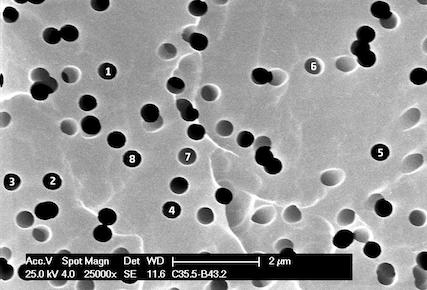
\includegraphics[scale=1.5]{Figures/115_numbered.png}
\caption{Mittlerer Kontrast und Helligkeit in 25.000-facher Vergrößerung}
\label{fig:appendix1}
\end{figure}
\hfill
\begin{figure}
\centering
	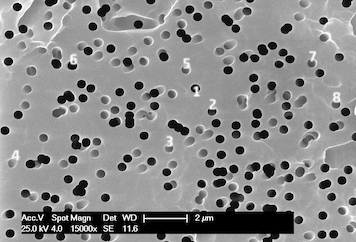
\includegraphics[scale=1.8]{Figures/101_numbered.png}
\caption{Mittlerer Kontrast und Helligkeit in 15.000-facher Vergrößerung}
\label{fig:appendix2}
\end{figure}
\hfill
\begin{figure}
\centering
	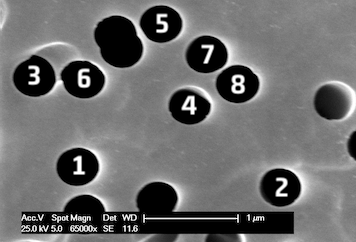
\includegraphics[scale=1.8]{Figures/100_numbered.png}
\caption{Mittlerer Kontrast und Helligkeit in 65.000-facher Vergrößerung}
\label{fig:appendix3}
\end{figure}

\end{document}